%%% Add [final] option to the report class to switch between draft and final version of the report
%%% Use [narrowmargin] to enable narrow margins - this may impair readability.
\documentclass[narrowmargin,12pt,a4paper,final]{include/intocpsassociation}   %Or intocpslargereport if chapters are required.

\usepackage[T1]{fontenc}
\usepackage[utf8]{inputenc}
\usepackage{longtable}
%\usepackage{tikz-uml}
\usepackage{multirow}
\usepackage{framed}
\usepackage{xcolor}
\usepackage{rotating}
\usepackage{subfigure}
\usepackage{amsmath}

\def\draftnote#1{\noindent\smallskip\framebox{\begin{minipage}{0.95\columnwidth}\color{red}#1\end{minipage}}\smallskip\par}
\newenvironment{draftnoteenv}{\noindent\smallskip\begin{framed}\begin{minipage}{0.95\columnwidth}\color{red}}{\end{minipage}\end{framed}\smallskip\par}
\newenvironment{assumption}{\noindent\smallskip\color{blue}\begin{framed}\begin{minipage}{0.95\columnwidth}}{\end{minipage}\end{framed}\smallskip\par}

\def\SG{Smart Grid}

\usepackage{listings}
\lstdefinestyle{cstyle}{basicstyle=\scriptsize\ttfamily,
			frame=trbl,
			showstringspaces=false,
			captionpos=b,
			frameround=tttt,
			aboveskip=5mm,
			belowskip=5mm,
			breaklines=true,
			tabsize=4,
			framexleftmargin=0mm,
			framexrightmargin=0mm}
\lstnewenvironment{config}{\lstset{style=cstyle}\lstset{language=sh}}{}

% for Celsius symbol
\usepackage{textcomp}

%%%%%%%%%%%%%%%%%%%%%%%%%%%%%%%%%%%%%%%%%
% New Command for text
%%%%%%%%%%%%%%%%%%%%%%%%%%%%%%%%%%%%%%%%%%
% shortcut for typewriter
\newcommand{\T}[1]{\texttt{#1}} % \T is defined in 
% shortcut for bold text
\newcommand{\B}[1]{\textbf{#1}}
\newcommand{\I}[1]{\textit{#1}}
\newcommand{\BI}[1]{\textit{\textbf{#1}}}
\newcommand{\TN}[1]{\textnormal{#1}}
\newcommand{\TTR}[1]{\textrm{#1}}
\newcommand{\mi}{\;|\;}
\newcommand{\ee}{&\quad::=\quad&}

\newcommand{\mrm}[1]{\mathrm{#1}} %Roman Font
\newcommand{\mbf}[1]{\mathbf{#1}} %Boldface Font
\newcommand{\msf}[1]{\mathsf{#1}} %Sans Serif Font
\newcommand{\mtt}[1]{\mathtt{#1}} %Typewriter Font
\newcommand{\miit}[1]{\mathit{#1}} %Italic Font
\newcommand{\mcl}[1]{\mathcal{#1}} %Calligraphic Front
\newcommand{\mnm}[1]{\mathnormal{#1}} %Normal Font

%\reportnumber{D3.6}
\reporttitle{The INTO-CPS Examples Compendium}
\shortreporttitle{Examples Compendium}  %To use if report title is too long for header

%%% Set document release class as appropriate
%%% e.g. Public, Restricted, Programme Participant
\reportstatus{Public}


%%% If document is a deliverable, this flag should be commented out
%%% e.g. %\technotetrue
%%% If report is a technical report, leave uncommented
%%% e.g. \technotetrue
%\technotetrue % Comment out as appropriate

\submissiondate{October 2018}
\contributors{
Richard Payne, UNEW\\
Carl Gamble, UNEW\\
Ken Pierce, UNEW\\
John Fitzgerald, UNEW\\
Martin Mansfield, UNEW\\
Simon Foster, UY\\
Kangfeng Ye, UY\\
Casper Thule, AU\\
Rene Nilsson, AU\\
Kenneth Lausdahl, AU\\
Florian Lapschies, VSI\\
Frederik Foldager, AI\\}

\editors{
John Fitzgerald, UNEW}

%\reviewers{
%Peter Gorm Larsen, AU\\
%Etienne Brosse, ST\\
%Adrian Pop, LIU}

%% Version details
% #1: version
% #2: date
% #3: author
% #4: description
\addversion{0.1}{15-05-2017}{Richard Payne}{Draft structure of deliverable and initial reframing based on D3.5}
\addversion{0.2}{27-10-2017}{Martin Mansfield}{Added Autonomous Vehicle and Mass Spring Damper pilots}
\addversion{0.3}{01-11-2017}{Martin Mansfield}{Version for internal review}
\addversion{1.0}{14-12-2017}{Martin Mansfield}{Review comments addressed}
\addversion{1.1}{26-02-2018}{Peter Gorm Larsen}{initial version for the INTO-CPS Association}
\addversion{1.2}{07-10-2018}{John Fitzgerald}{Alignment with other Association documents}
\addversion{1.3}{02-11-2018}{Casper Thule}{Updated example links}


\begin{document}
\maketitle

%%%% Document abstract page %%%%
\section*{Abstract}
\label{sec:abstract}

This document is intended for users of the INTO-CPS technologies and contains a collection of example and pilot study model descriptions demonstrating the INTO-CPS technology. Each study has a description of the example, the models available for the study and examples of the analyses available with the INTO-CPS Tool Chain. The examples demonstrate the INTO-CPS tools developed during (and after) the INTO-CPS project. This compendium is a living document that has grown with the tool chain. This document is a snapshot of the compendium presently, building on previous versions (in M12~\cite{INTOCPSD3.4}, M24~\cite{INTOCPSD3.5} and M36~\cite{INTOCPSD3.6}). The latest version can always be found at \url{https://github.com/INTO-CPS-Association/training/releases}.

\newpage

%%%% Document table of contents page %%%%
\tableofcontents
\newpage

% !TeX root = D3.5_Examples_Compendium_2.tex
% !TeX spellcheck = en_GB

\section{Introduction}\label{sec:intro}

This document provides an overview of different public example multi-models that stakeholders who are interested in experimenting with the INTO-CPS technology can use as a starting point. The examples have been developed using the different simulation technologies in INTO-CPS: 20-sim\footnote{\url{http://www.20sim.com}}; Overture/VDM-RT\footnote{\url{http://overturetool.org}}; OpenModelica\footnote{\url{https://openmodelica.org}}; SysML\footnote{Using the Modelio tool: \url{https://www.modeliosoft.com}}; and RT-Tester\footnote{\url{https://www.verified.de/products/rt-tester/}}). The examples are  comprised of multi-models using the INTO-CPS SysML profile and collections of Continuous Time (CT) and Discrete Event (DE) models elicited from the simulation models. Examples of their use is also given, demonstrating features and analyses made available by the INTO-CPS tool chain. 

This deliverable is structured in different sections, each of which provides a brief introduction to each example model. Each example illustrates different aspects of the INTO-CPS tool chain, as summarised here:

\begin{itemize}
  \item Section~\ref{sec:singletank} presents a Single-tank Water Tank model. The simplest example in the compendium, this is a two-model multi-model, using 20-sim and VDM-RT FMUs.  The example has a SysML architecture, can be co-simulated, and has support for Design Space Exploration (DSE).
  \item Section~\ref{sec:threetank} presents a Three-tank Water Tank model. This study aims to demonstrate the division of CT elements across different FMUs. The study comprises 20-sim and VDM-RT FMUs and demonstrates DSE and Test Automation technologies. 
  \item Section~\ref{sec:fcu} presents a Fan Coil Unit (FCU). Originally presented as a baseline OpenModelica model. This model demonstrates the options for multi-modelling and dividing models into separate FMUs to allow for architecting to be carried out in the SysML architectural model. The example demonstrates the use of co-simulation and DSE.
  \item Section~\ref{sec:linefollwerrobot} presents a Line-following Robot. This study has four possible co-simulation multi-models -- two using replication offered by 20-sim FMUs (one using 3D visualisation and one without) and another two configurations which are not using FMU replication. The study provides several DSE experiments.
  \item Section~\ref{sec:turn} presents a Turn Indicator example.
  In this study, the behaviour of a car's turn indicator is modelled using parallel state-charts.
  This model is then used to automatically derive tests and to perform model checking.
  \item Section~\ref{sec:uavsingle} presents a single-UAV model, which models the physical dynamics as well as the discrete controller of an Unmanned Aerial Vehicle (UAV). The model contributes a high-fidelity physical model, enabling the multi-model to be used to compare alternative control algorithms.
  \item Section~\ref{sec:ether} presents an Ether communication model. This pilot provides an initial demonstration of a model for network communications. This pilot is VDM-RT only, with a simple SysML architecture. Co-simulation takes the form of the demonstration of messages passing through the ether. The intention is that this pilot will be used in the future by others using network communications. 
  \item Section~\ref{sec:uavswarm} presents a swarm of communicating simplified UAVs. This pilot is a first version of a swarm of UAVs which receive direction from a central controller. The pilot uses FMUs from 20-sim and VDM-RT taking advantage of FMU replication offered by both notations. Co-Simulation and 3D visualisation are supported.
 % \item Section~\ref{sec:smartgrid} presents a smart grid multi-model. This study is a preliminary study presenting only the architecture and constituent models in 20-sim and VDM-RT. FMUs have not yet been produced, therefore co-simulation has yet to be demonstrated.
  \item Section~\ref{sec:bicycle} presents an autonomous vehicle model. In this study, a multi-model demonstrates a vehicle traversing a path of defined waypoints. The multi-model comprises two FMUs; The dynamics of the vehicle are modelled by a 20-sim FMU, and the vehicle control is determined by a VDM-RT FMU. The example has a SysML architecture, can be co-simulated, and has support for DSE.
  \item Section~\ref{sec:massspringdamper} presents a mass spring damper model. The pilot uses models of masses and springs to demonstrate the utility of so-simulation stabilisation using both 20-sim and OpenModelica FMUs.
 
  
\end{itemize}

In order to guide you in what models to consider inspecting, we have created Table~\ref{tab:into_examples} illustrating the different characteristics of the different publicly available models. 

\begin{table}[ht]
\begin{centering}
\begin{tabular}{|l|c|c|c|c|c|c|c|c|c|c|c|}\hline
  &\multicolumn{11}{c|}{INTO-CPS Technology} \\
\cline{2-12}
Model
%&\begin{sideways}Single DE Model\end{sideways}
%&\begin{sideways}Single CT Model\end{sideways}
%&\begin{sideways}`Holistic' SysML model\ \end{sideways} 
&\begin{sideways}Multi-DE model\end{sideways}
&\begin{sideways}Multi-CT model\end{sideways}
&\begin{sideways}20-Sim (for FMU)\end{sideways}
&\begin{sideways}OpenModelica (for FMU)\end{sideways}
&\begin{sideways}VDM-RT (for FMU)\end{sideways}
&\begin{sideways}INTO-CPS SysML\end{sideways}  
&\begin{sideways}Co-simulation engine(COE)\end{sideways}
%&\begin{sideways}\textcolor{gray}{SysML requirements}\end{sideways}
%&\begin{sideways}Traceability links identified\end{sideways}
&\begin{sideways}DSE support included\end{sideways}
&\begin{sideways}{Test Automation support}\end{sideways}
&\begin{sideways}{Model checking}\end{sideways}
&\begin{sideways}{Code Generation}\end{sideways} \\
\hline
Single-tank Water Tank	& & &x&x&x&x&x&x& & &x\\ \hline
Three-tank Water Tank	& &x&x& &x&x&x&x&x& &x\\ \hline
Fan Coil Unit (FCU)		& &x&x&x&x&x&x&x&x&x&x\\ \hline
Line-following Robot		& &x&x&x&x&x&x&x&x&x&x\\ \hline
Turn Indicator			& & & & & & & & &x&x&\\ \hline
\rowcolor{lightRed} Single UAV & &x&x& &x&x&x& & & &\\ \hline
Ether				&x& & & &x& &x& &x&x& \\ \hline
UAV Swarm			&x&x&x& &x&x&x& &x&x&\\ \hline
%Smart Grid			&x&x&x& &x&x& & & & &\\ \hline
Autonomous Vehicle			& & &x& &x&x&x&x& & &\\ \hline
Mass Spring Damper			& & &x&x& & &x& & & &\\ \hline
\end{tabular}
\caption{Overview of INTO-CPS technologies used for pilot studies. An unmaintained model is marked with {\textcolor{lightRed}{\rule{1em}{1em}}}}
\label{tab:into_examples}
\end{centering}
\end{table}
%%% Local Variables:
%%% mode: latex
%%% TeX-master: "INTO-CPS_Examples_Compendium"
%%% End:

\clearpage
\section{Single-tank Water Tank}
\label{sec:singletank}

\subsection{Example Description}
\label{sec:singletank_desc}

The single-tank water tank pilot study is a simple example that comprises a single water tank which is controlled by a cyber controller. When the water level of the tank reaches a particular level (defined in the controller) the controller sends a command to the tank to empty using an exit valve. A diagram of the example is shown in Figure~\ref{fig:singletankoverview}. 
This pilot is also related to the next pilot in Section~\ref{sec:threetank}. 

\begin{figure}[htbp]
\begin{center}
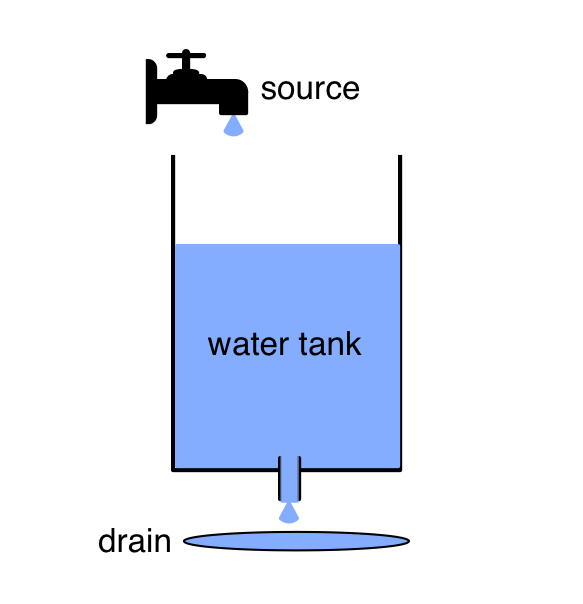
\includegraphics[width=0.4\textwidth]{singletank/singletank}
\caption{Overview of the single-tank water tank example}
\label{fig:singletankoverview}
\end{center}
\end{figure}

\subsection{Usage}
\label{sec:singletank_usage}

The example is available from the INTO-CPS application menu at \emph{File>Import Example Project} or at \url{https://github.com/INTO-CPS-Association/example-single_watertank} in the \emph{master} branch. There are several subfolders for the various elements: \texttt{FMU} contains the various FMUs of the study; \texttt{Models} -- contains the constituent models defined using the INTO-CPS simulation technologies; \texttt{Multi-models} -- contains the multi-model definition;  and \texttt{SysML} -- contains the SysML model defined for the study.

The \texttt{case-study\_single\_watertank} folder can be opened in the INTO-CPS application to run the various co-simulations as detailed in this document. To run a simulation, expand one of the multi-models and click `Simulate' for an experiment. 

%\subsection{INTO-CPS Technology}
%\label{sec:singletank_into}
%
%
%We demonstrate the use of the INTO-CPS SysML profile in Section~\ref{sec:singletank_into_sys}. Based upon the design architecture defined using the SysML profile, a multi-model is constructed in Section~\ref{sec:singletank_into_mm} along with the defined connections. The study is also used to demonstrate the Co-Simulation Orchestration Engine (COE) in Section~\ref{sec:singletank_into_co}. 

\subsection{INTO-CPS SysML profile}
\label{sec:singletank_into_sys}

The single tank SysML model produced using the INTO-CPS profile comprises two diagrams; an Architecture Structure Diagram (ASD) and a Connections Diagram (CD). 

The ASD in Figure~\ref{fig:fig:singletankasd} shows the system composition in terms of component subsystems from the perspective of multi-modelling. 

\begin{figure}[htbp]
\begin{center}
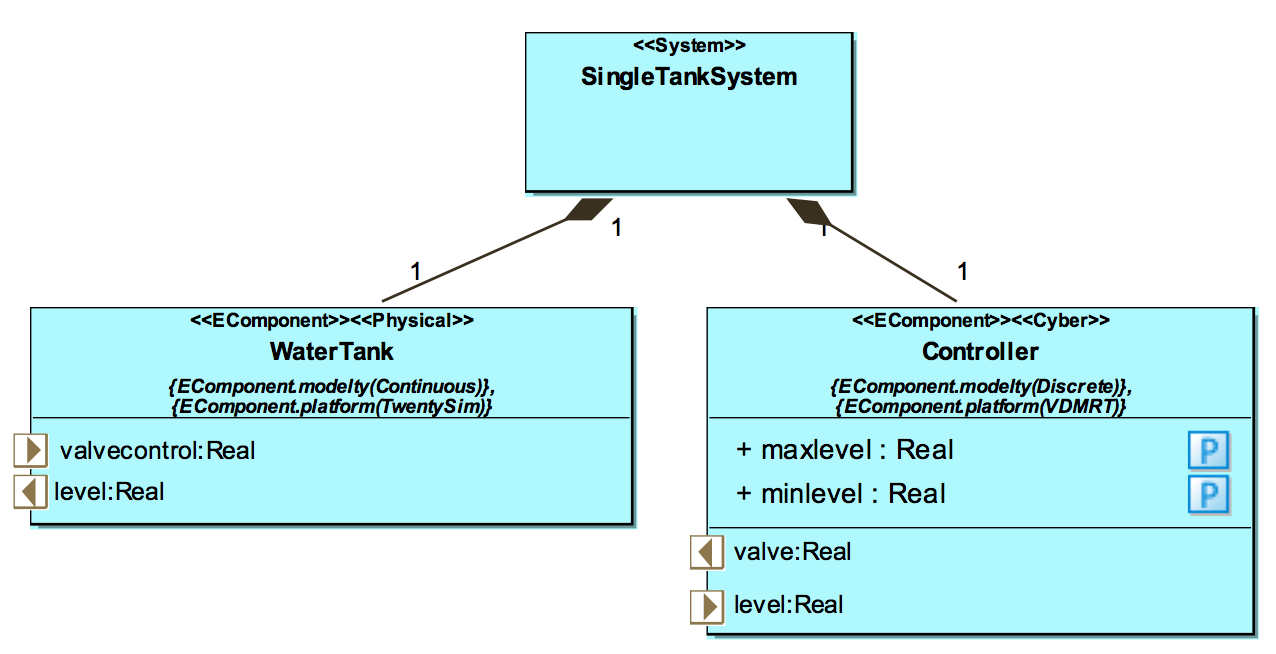
\includegraphics[width=0.8\textwidth]{singletank/sysml_asd.png}
\caption{Architecture Structure Diagram defining the Single-tank Water Tank system composition}
\label{fig:fig:singletankasd}
\end{center}
\end{figure}

This \emph{SingleTankSystem} model, comprises  a single \emph{WaterTank} physical component and  a cyber component \emph{Controller}. Ports are exposed by the  \emph{WaterTank} component for outputting the current water level (\texttt{level}) and for receiving valve control commands (\texttt{valvecontrol}). The \emph{Controller} component has reciprocal ports and also variables to define the permitted minimum and maximum water levels (\texttt{minlevel} and \texttt{maxlevel} respectively).

The \emph{WaterTank} component is defined as a continuous time model with 20-sim as the target platform, this may be also be defined as OpenModelica. The \emph{Controller} component is a VDM-RT discrete event model. 

A single System Block Instance is defined in the model to represent the system configuration. The CD in Figure~\ref{fig:singletankcd} shows that the \emph{WaterTank} component has two connections with the \emph{Controller} cyber component - regarding the level and valve control.

\begin{figure}[htbp]
\begin{center}
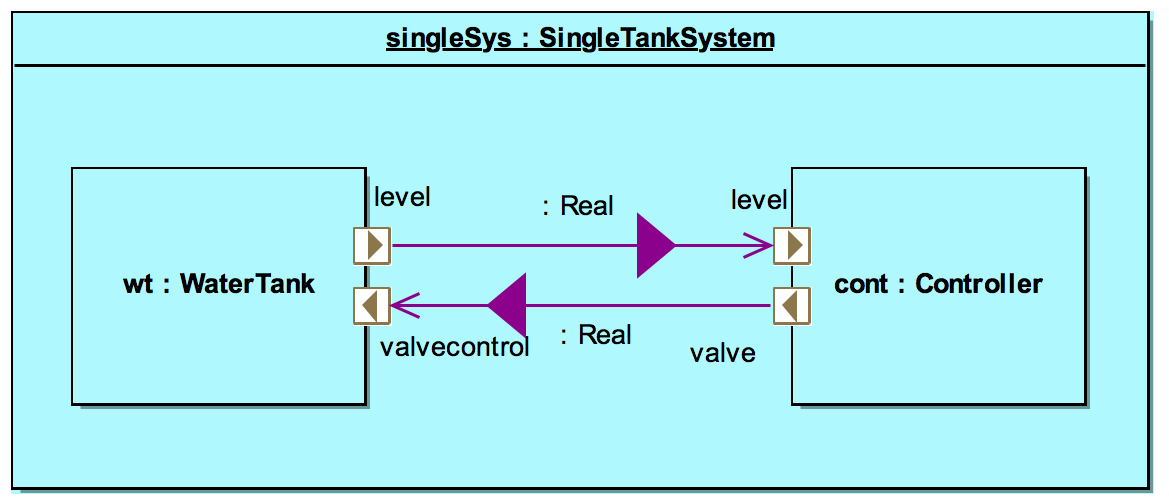
\includegraphics[width=0.75\textwidth]{singletank/sysml_cd.png}
\caption{Connections Diagram defining the Single-tank Water Tank system connections}
\label{fig:singletankcd}
\end{center}
\end{figure}

\subsection{Multi-model}
\label{sec:singletank_into_mm}

\subsubsection{Models}
\label{sec:singletank_into_models}

The SysML model above dictates there are two models: a 20-sim model for the water tank and a VDM-RT model for the controller. This section gives an overview of those models.

\begin{description}
\item[Watertank.emx] The 20-sim model of the \emph{Water Tank} component, shown in Figure~\ref{fig:singletank20-sim}, comprises several sub-components. A flow source is connected to a tank, which fills up at a constant rate. The tank reports the current water level on the \emph{level} port. A valve, controlled by the \emph{valvecontrol} port empties water from the tank into a drain.

\begin{figure}[htbp]
\begin{center}
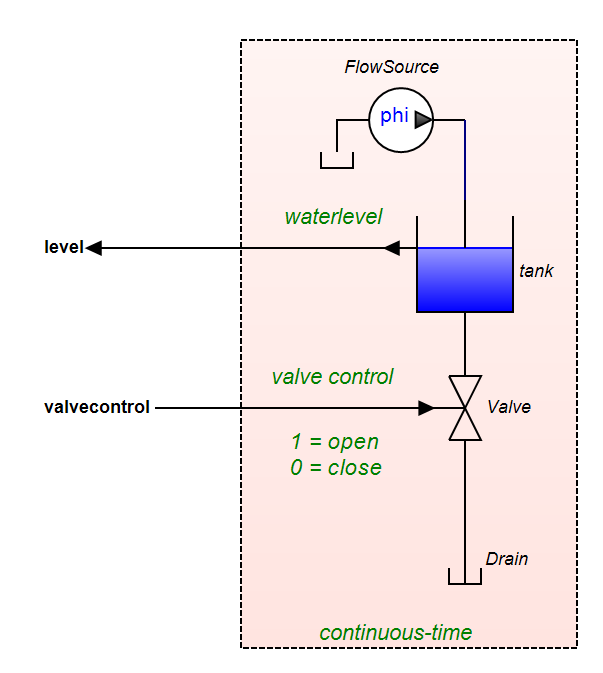
\includegraphics[width=0.5\textwidth]{singletank/20-sim.png}
\caption{20-sim Water Tank component}
\label{fig:singletank20-sim}
\end{center}
\end{figure}

\item[WaterTank.mo] \emph{WaterTank.mo} contains a \emph{SingleWaterTank} model, which has the same external interface as the above \emph{SingleWatertank.emx} model -- as both comply to the FMI \emph{modeldescription.xml} exported format. The model is defined mainly through equations, and so is not shown in this document.
%
%\begin{figure}[htbp]
%\begin{center}
%To Appear %\includegraphics[width=0.5\textwidth]{singletank/om.png}
%\caption{OpenModelica Water Tank component}
%\label{fig:singletankom}
%\end{center}
%\end{figure}

\item[SingleWT] The VDM-RT \emph{SingleWT} controller is a simple model, with an architecture shown in Figure~\ref{fig:singletank20-vdm}. The \emph{System} class owns a \emph{HardwareInterface} instance with RealPorts to receive the sensed water level and send valve control commands. The values are passed to \emph{LevelSensor} and \emph{ValveActuator} objects used by the \emph{Controller} class. The control algorithm compares the level to the \emph{minlevel} and \emph{maxlevel} design parameters and sets the valve control appropriately.
 
\begin{figure}[htbp]
\begin{center}
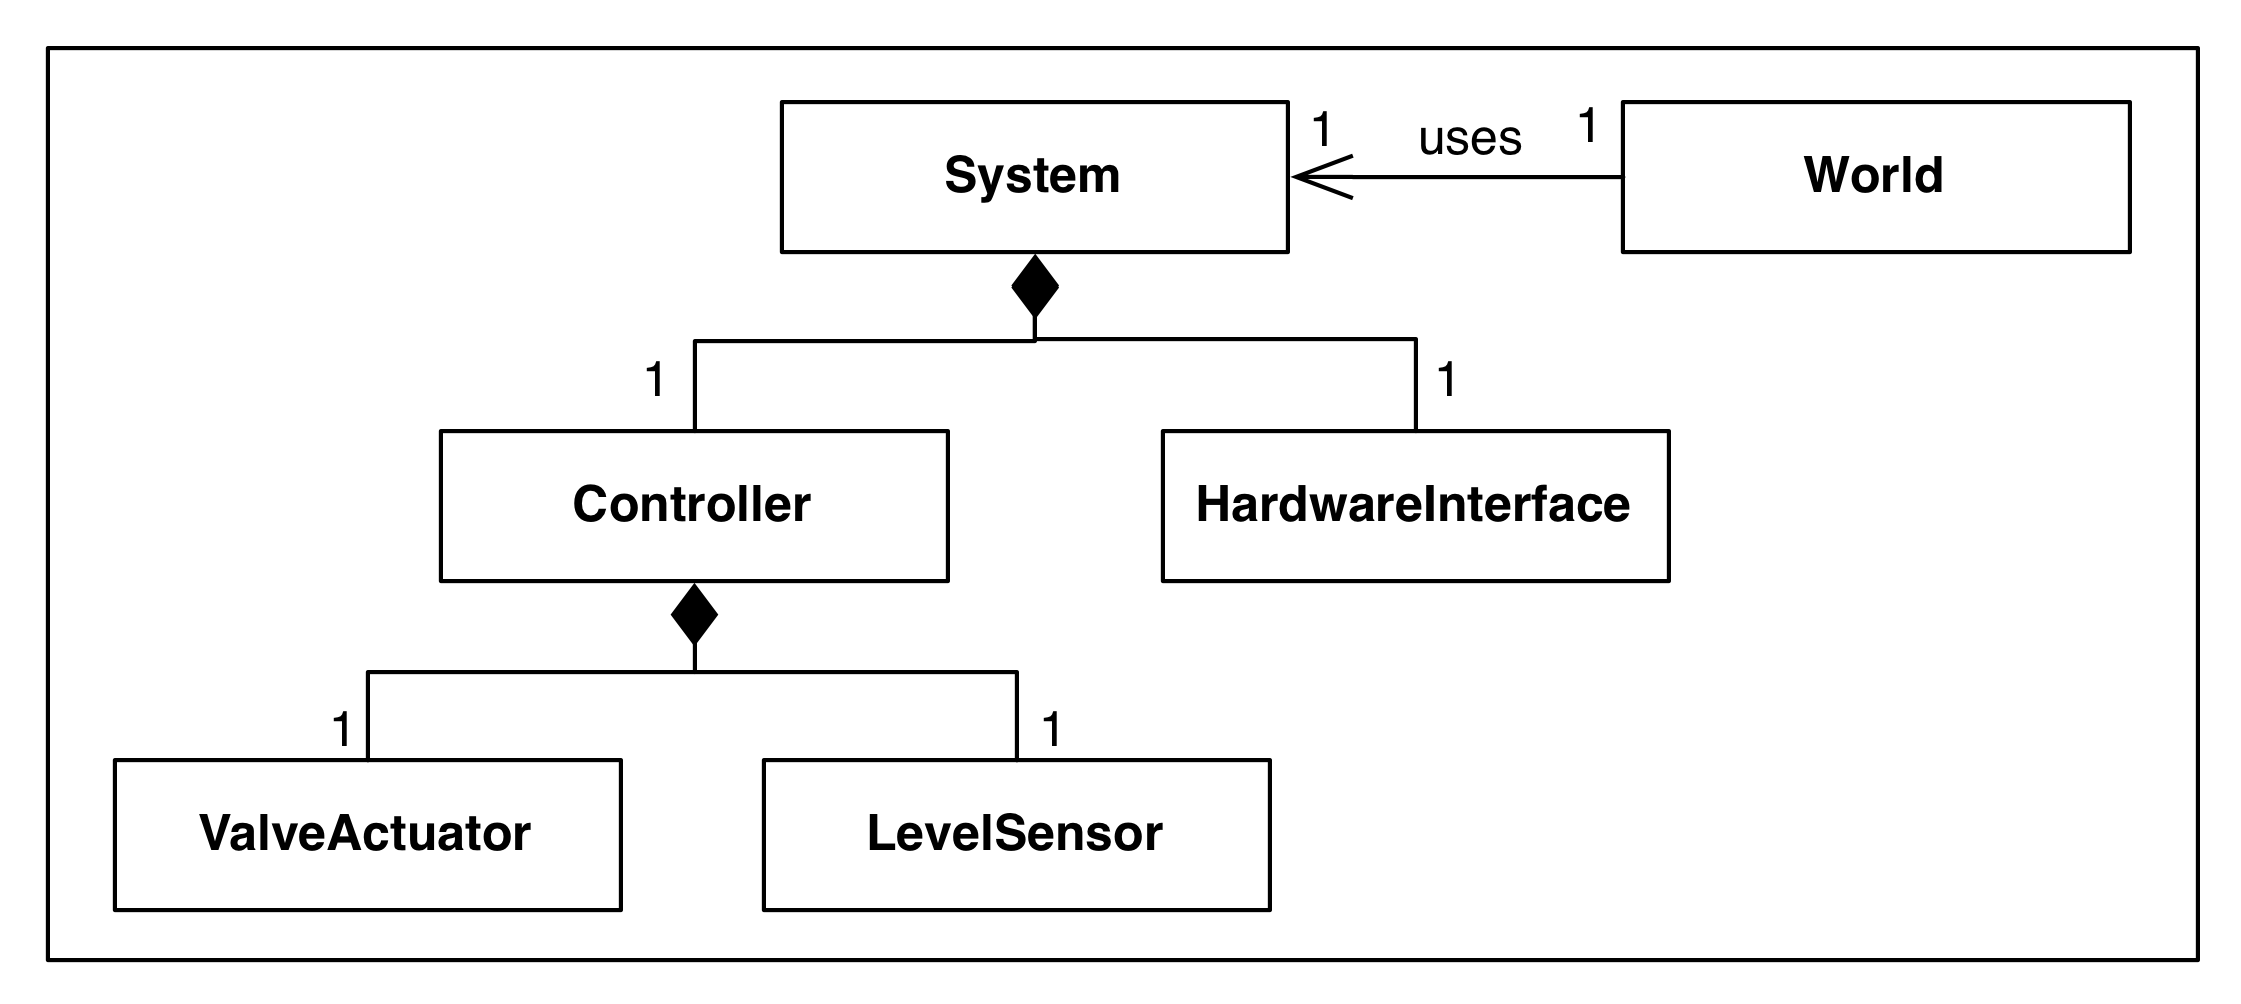
\includegraphics[width=0.755\textwidth]{singletank/vdmrtarch.png}
\caption{VDM-RT model architecture}
\label{fig:singletank20-vdm}
\end{center}
\end{figure}

\end{description}

\subsubsection{Configuration}
\label{sec:singletank_into_conf}
Two multi-models are defined:
\begin{description}
\item[mm] The multi-model \texttt{mm} corresponds to the CD in Section~\ref{sec:singletank_into_sys}. Two connections are defined:

\begin{itemize}
  \item from the \emph{WaterTank} \texttt{level} port to the \emph{Controller} \texttt{level} port; and 
  \item from the \emph{Controller} \texttt{valve} port to the \emph{WaterTank} \texttt{valvecontrol} port. 
\end{itemize}

The FMUs used are \emph{singlewatertank-20sim.fmu} and \emph{SingleWT.fmu}

There are two design parameters in the multi-model -- \texttt{minlevel} and \texttt{maxlevel}, which are defined to be 1.0 and 2.0 respectively. 

\item [mm-OM] An alternative multi-model is defined using the OpenModelica FMU. The connections are identical to the multi-model above, although rather than using the 20-sim FMU, \emph{WaterTank\_SingleWaterTank.fmu} is used.

\end{description}

\subsection{Co-simulation}
\label{sec:singletank_into_co}

A co-simulation experiment is defined for the multi-model -- with a runtime of 30 seconds and using the fixed step size of 0.1 seconds. Simulating using this experiment produces the livestream output shown in Figure~\ref{fig:cosim-graph}.

\begin{figure}[htbp]
\begin{center}
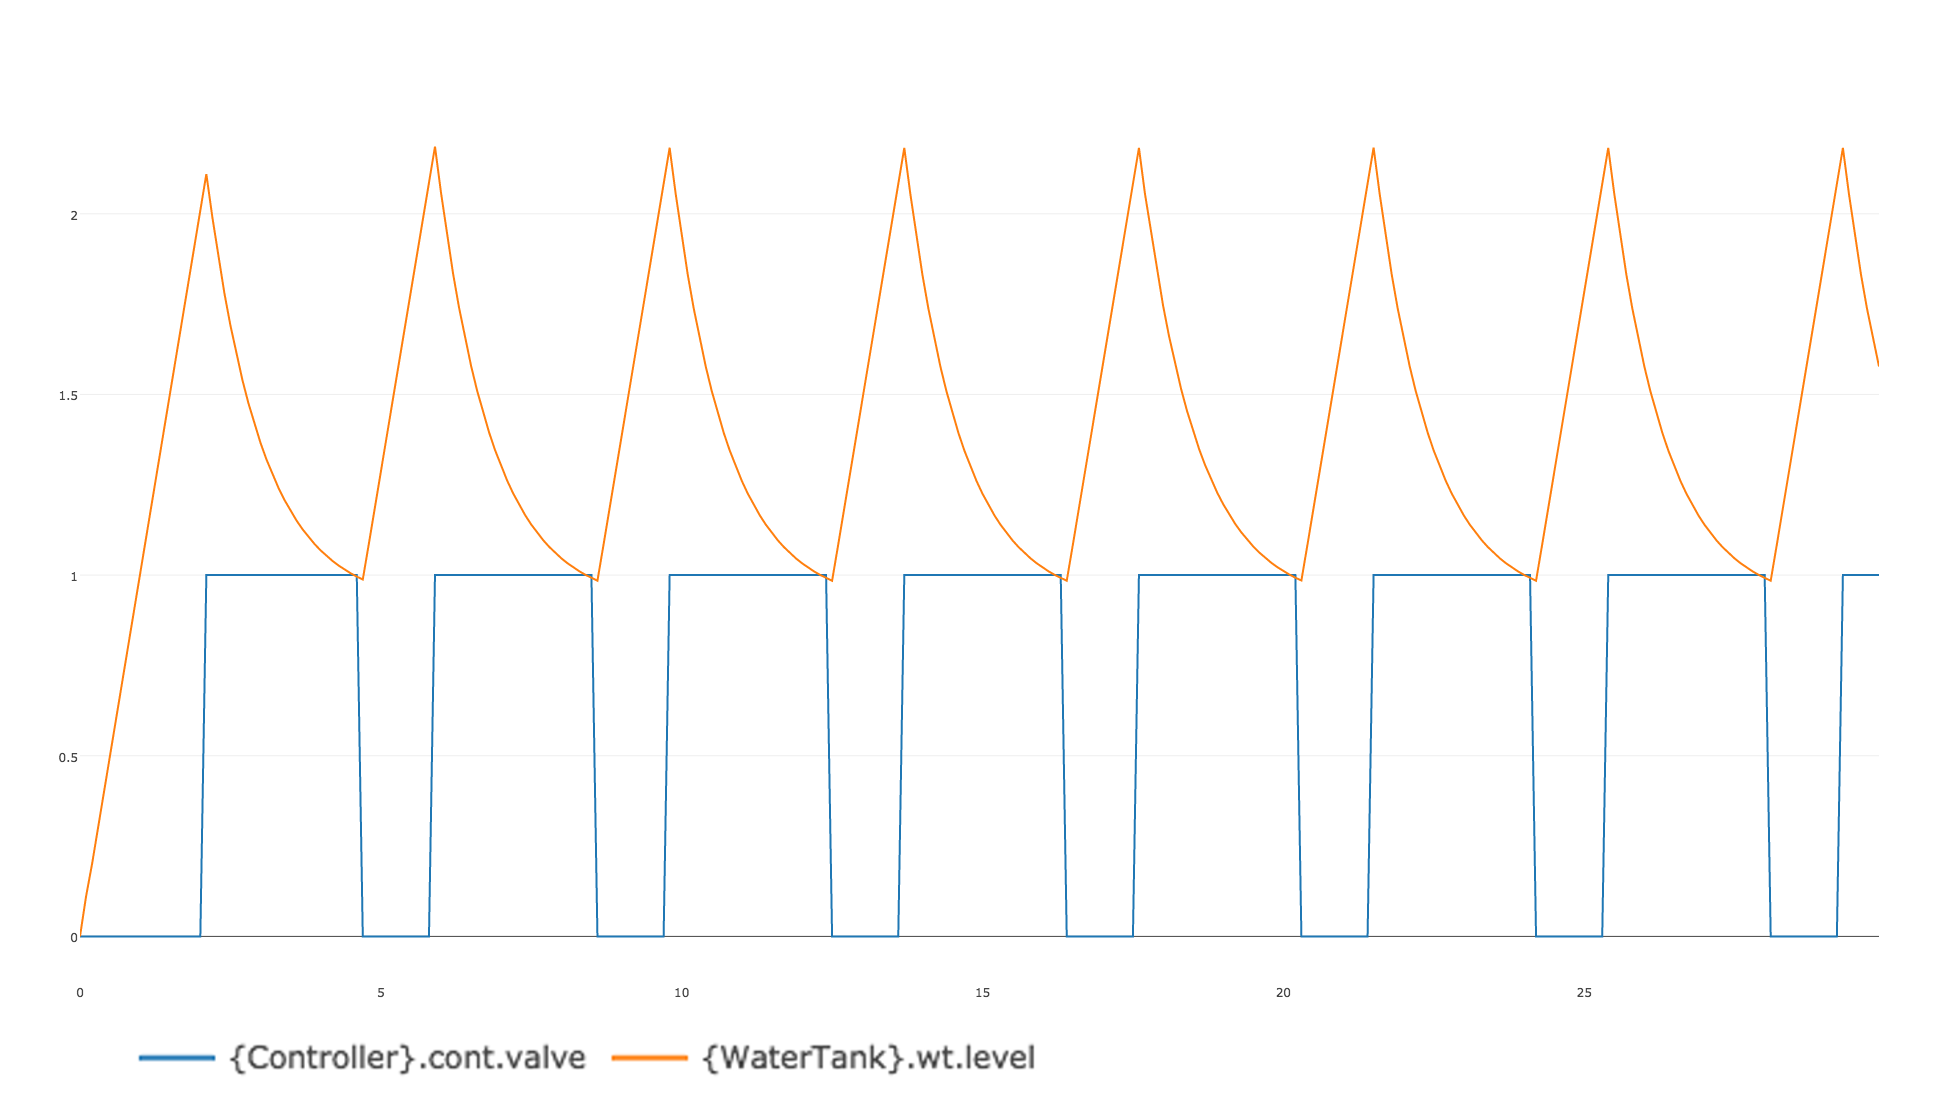
\includegraphics[width=1\textwidth]{singletank/cosim-results.png}
\caption{Co-simulation results for Single-tank Water Tank system}
\label{fig:cosim-graph}
\end{center}
\end{figure}

The graph shows the water level (orange line) and valve control (blue line) values. The water level rises steadily until it reaches 2.0 (the maximum level), at this point the valve control is set to 1.0 and the water level drops to 1.0 (the minimum level). At the minimum level, the valve is closed and the water rises once again. This behaviour repeats through to the end of the simulation. 

\subsection{Analyses and Experiments}

\subsubsection{Design Space Exploration}
\label{sec:singletank_dse}

This pilot supports DSE. We reuse the DSE experiment used in the Three-tank Water Tank Pilot study -- and is briefly described here. For discussion on results obtained, see the Three Tank study in Section~\ref{sec:threetank_dse}.

The experiment varies the two design parameters of the study -- \texttt{minlevel} and \texttt{maxlevel}. These parameter values may be set between $0.2$ and $2.0$ in intervals of $0.2$. A constraint on the parameters (\texttt{{Controller}.cont.maxlevel $>$ {Controller}.cont.minlevel}) ensures that the maximum water value is always larger than the minimum water level. 

Two objectives are defined: \textit{cumulativeDeviation} and \textit{vCount}. The first objective, \textit{cumulativeDeviation}, is to minimise the cumulative deviation from a desired level - set to $1.0$. The second objective, \textit{vCount}, is to minimise the number of valve operations -- i.e. have a lower number of valve state changes. The analysis uses the Pareto method for ranking.

\subsubsection{Code Generation}

The VDM-RT model, \textbf{SingleWT} can be exported from Overture as a C code FMU, in addition to the tool wrapper FMU as used above. The \emph{watertankController-SourceCode.FMU} included in this pilot is obtained directly from Overture using the ``Export Source Code FMU'' option. However, this FMU does not contain binaries for co-simulation and so one may use the \emph{FMU Builder} included in the INTO-CPS Application to compile FMUs for Windows, Mac and Linux. 

This process has been performed and the resultant FMU is included in the pilot in the FMUs folder; \emph{watertankController-Standalone.FMU}. One example experiment available is to switch this FMU for the tool wrapper version -- \emph{SingleWT.FMU} -- and compare results. 
\clearpage
\section{Three-tank Water Tank}
\label{sec:threetank}
%\fbox{LIU: OpenModelica Watertanks not available.}


\subsection{Example Description}
\label{sec:threetank_desc}

The three-tank water tank model is based upon a standard 20-sim example, and is developed to explore the impact on accuracy of multi-modelling across multiple CT models. The example comprises three water tanks which are filled and emptied. The first tank is filled from a source with a valve which may be turned on and off. The outflow of the first tank constitutes the inflow of the second, and so forth. A controller monitors the level of the third tank and controls a valve to a drain. 

A key feature of this example is the close coupling required between water tank 1 and 2, and the loose coupling to water tank 3. Water tanks 1 and 2 are tall and thin and are connected by a pipe at the bottom of the tanks (a diagram of the example is shown in Figure~\ref{fig:threetankoverview}), and therefore changes to the level of water tank 1 (due to water entering from the source) will quickly affect the level in water tank 2. This effect is not as prevalent between water tank 2 and 3. 


\begin{figure}[htbp]
\begin{center}
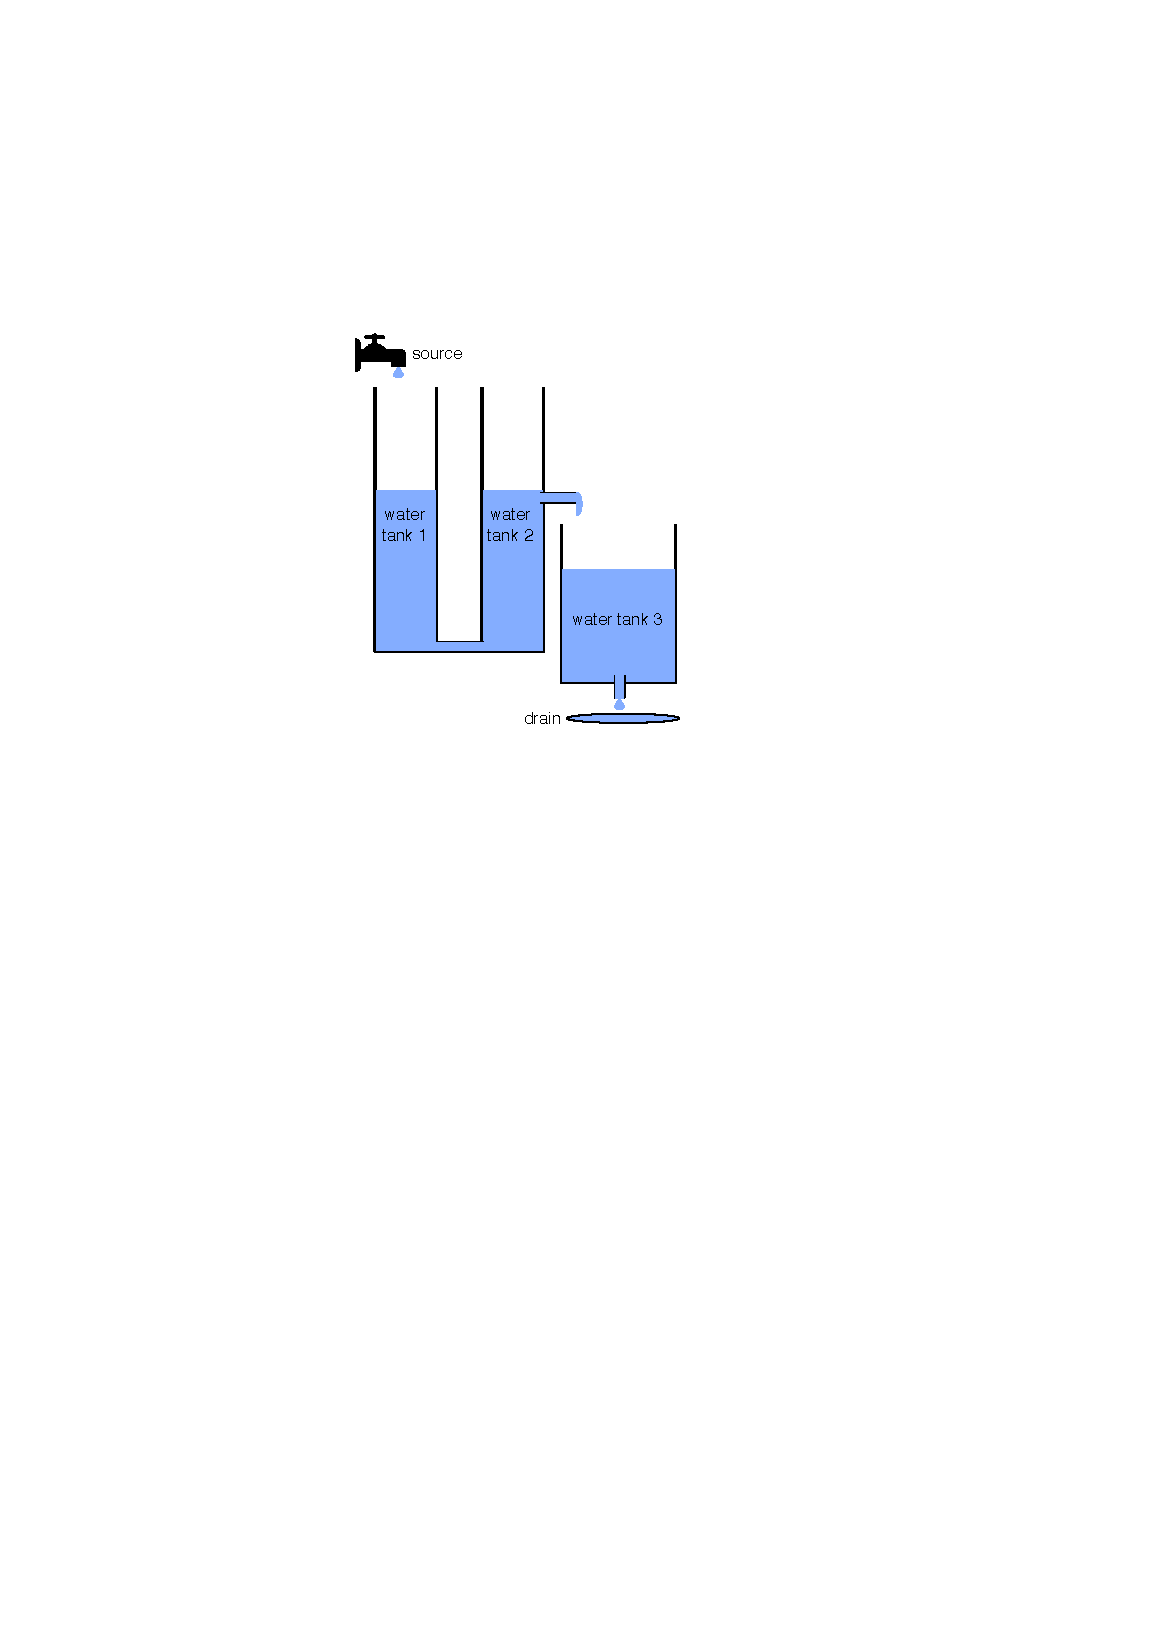
\includegraphics[width=0.5\textwidth]{threetank/ttwt_overview}
\caption{Overview of the three-tank water tank example}
\label{fig:threetankoverview}
\end{center}
\end{figure}

This pilot expands that in Section~\ref{sec:singletank}.

\subsection{Usage}
\label{sec:threetank_usage}

The example is available from the INTO-CPS application menu at \emph{File>Import Example Project} or at  \url{https://github.com/into-cps/case-study\_three\_tank} in the \emph{master} branch. There are several subfolders for the various elements: \texttt{DSEs} - contains work in progress DSE scripts; \texttt{FMU} -- contains the various FMUs of the study; \texttt{Models} -- contains the constituent models defined using the INTO-CPS simulation technologies; \texttt{Multi-models} -- contains the multi-model definitions and co-simulation configurations; \texttt{SysML} -- contains the SysML models defined for the study; resources -- various images for the purposes of this readme file. 

The \texttt{case-study\_three\_tank} folder can be opened in the INTO-CPS application to run the various co-simulations as detailed in this document. To run a simulation, expand one of the multi-models and click `Simulate' for an experiment. 


%\subsection{INTO-CPS Technology}
%\label{sec:threetank_into}
%
%We demonstrate the use of the INTO-CPS SysML profile in Section~\ref{sec:threetank_into_sys}. Based upon the design architecture defined using the SysML profile, a multi-model is constructed in Section~\ref{sec:threetank_into_mm} along with the defined connections. The study is also used to demonstrate the Co-Simulation Orchestration Engine (COE) in Section~\ref{sec:threetank_into_co}. % In Section~\ref{sec:threetank_3D} we outline the use of the INTO-SysML profile for visualisation of the model using a 20-sim FMU. 
%Section~\ref{sec:threetank_dse} outlines the use of the INTO-CPS DSE tool in the Three Tank model.

\subsection{INTO-CPS SysML profile}
\label{sec:threetank_into_sys}

A SysML model produced using the INTO-CPS profile comprises three diagrams and focusses on the structure of the water tank model for multi-modelling; an Architecture Structure Diagram and two Connections Diagrams. 

The Architecture Structure Diagram (ASD) in Figure~\ref{fig:threetankasd} shows the system composition in terms of component subsystems from the perspective of multi-modelling. As discussed in~\cite{INTOCPSD3.4}, this architecture differs from a holistic architecture due to the grouping of tanks into the different subsystems. 

\begin{figure}[htbp]
\begin{center}
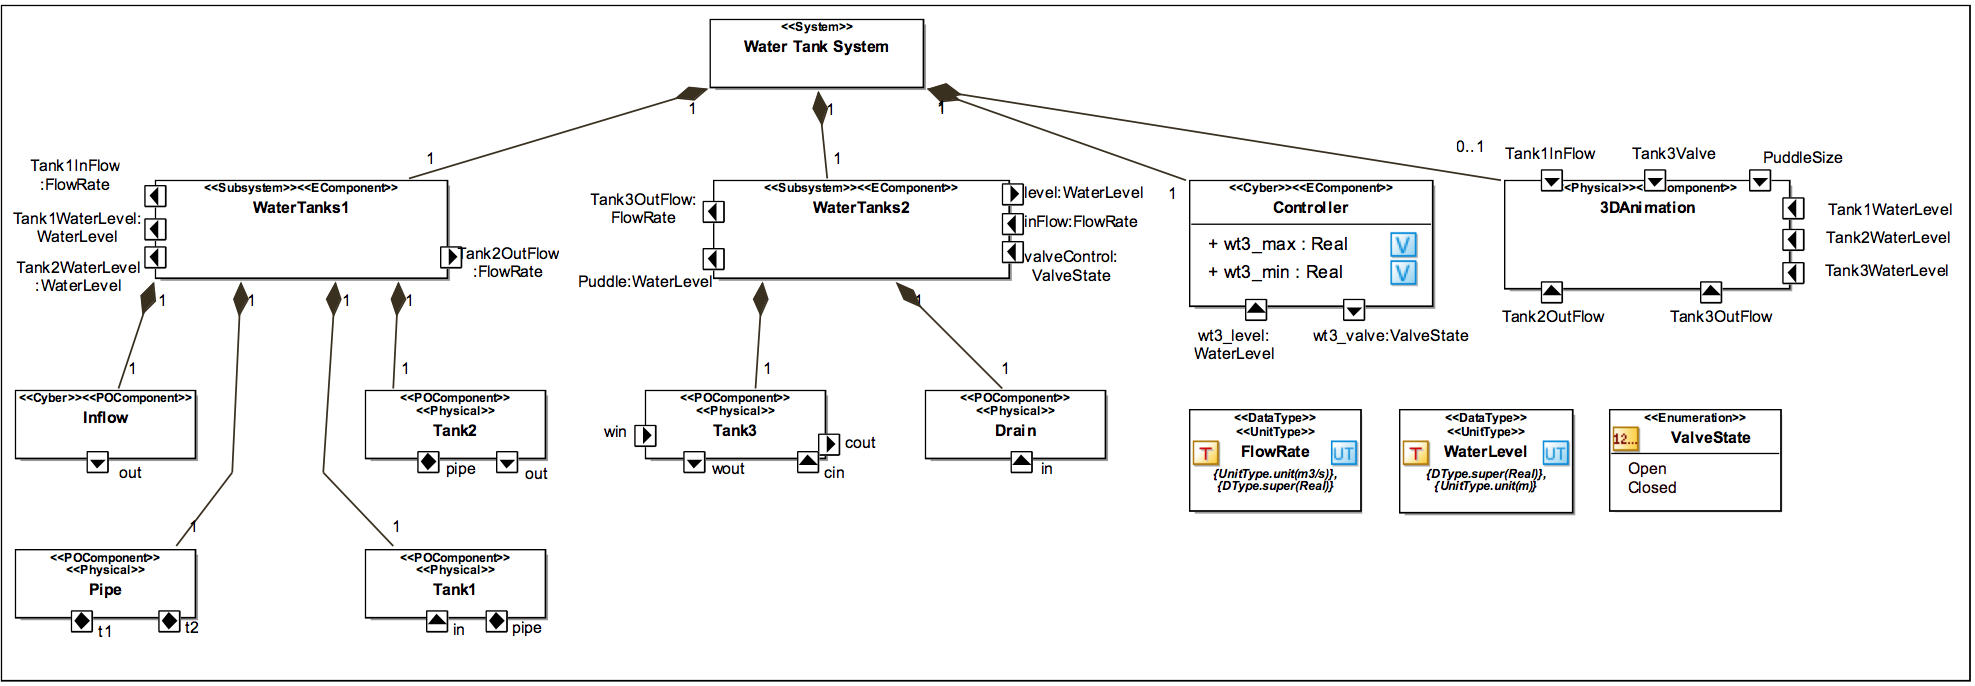
\includegraphics[width=1\textwidth]{threetank/ttwt_asd_vis.png}
\caption{Architecture Structure Diagram defining the Three-tank Water Tank system composition}
\label{fig:threetankasd}
\end{center}
\end{figure}

In this Water Tank system model, the water tanks are split between two subsystems: \emph{WaterTanks1} subsystem contains the \emph{Source}, two \emph{Water Tank} and  \emph{Pipe} components; \emph{WaterTanks2} subsystem comprises a single \emph{Water Tank} and \emph{Drain} components; a cyber component \emph{Controller} contains no other components; and the 3D component is available for visualising the behaviour of the system. 

To allow the visualisation FMU to depict the internal workings of the system's components, additional ports have been defined for the \emph{WaterTanks1} and  \emph{WaterTanks2} blocks. The \emph{WaterTanks1} component exposes: \texttt{Tank1InFlow} -- corresponding to the rate of water flowing into \emph{Tank1}; \texttt{Tank1WaterLevel} -- the water level of \emph{Tank1}; and \texttt{Tank2WaterLevel} -- the water level of \emph{Tank2}. The \emph{WaterTanks2} component exposes the additional ports: \texttt{Tank3OutFlow} -- corresponding to the rate of water flowing out of \emph{Tank3} and \texttt{puddle} -- the current volume of water in the drain (or puddle).

The two water tank subsystems are defined as continuous time models, both with 20-sim as the target platform. The controller component is a VDM-RT discrete event model. 

Two System Block Instances are defined in the model to represent alternative system configurations -- they are defined in separate Connections Diagrams (CDs). The CD in Figure~\ref{fig:threetankcd} defines connections as follows: at the subsystem-level,  the output of water from the \emph{WaterTanks1} subsystem is input to the \emph{WaterTanks2} subsystem. This subsystem has two connections with the \emph{Controller} cyber component - regarding the level and valve control.

\begin{figure}[htbp]
\begin{center}
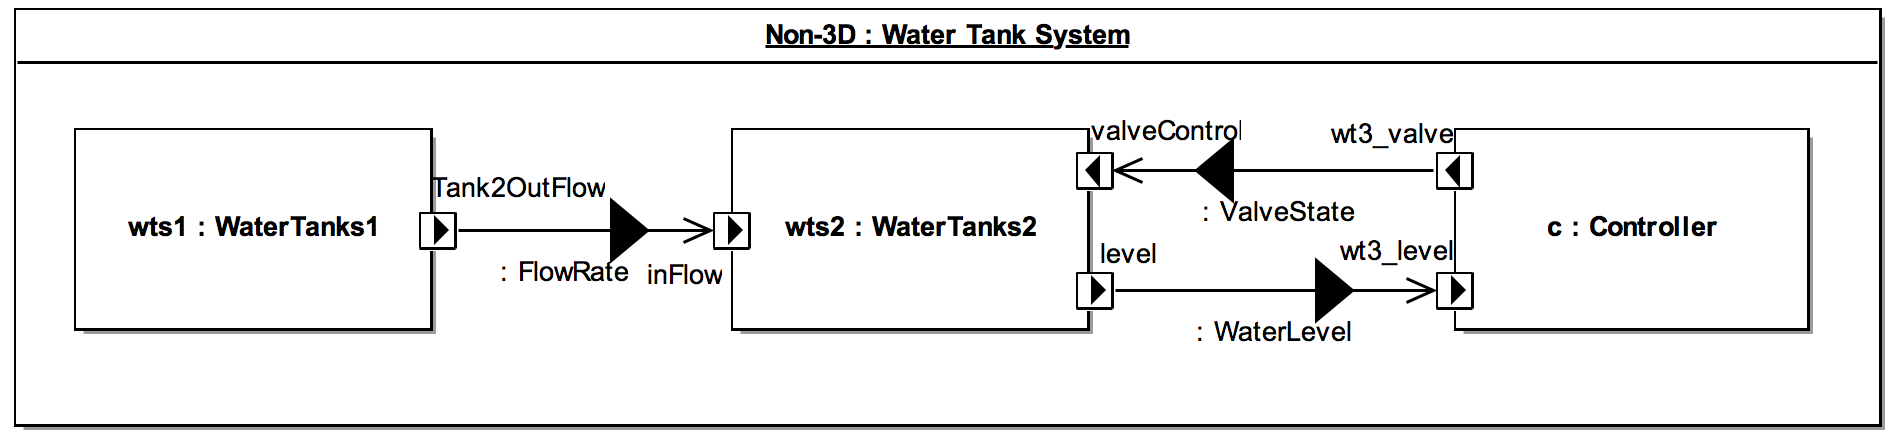
\includegraphics[width=0.85\textwidth]{threetank/ttwt_cd.png}
\caption{Connections Diagram defining the Three-tank Water Tank system connections}
\label{fig:threetankcd}
\end{center}
\end{figure}

 Figure~\ref{fig:threetankcdvis} depicts the second CD with several connectors between the system component instances and the 3D visualisation block instance. The connections in Figure~\ref{fig:threetankcd} are still present, with additional connections sending state information relating to tank water levels, flow rates and controller behaviour to the 3D model.
 
\begin{figure}[htbp]
\begin{center}
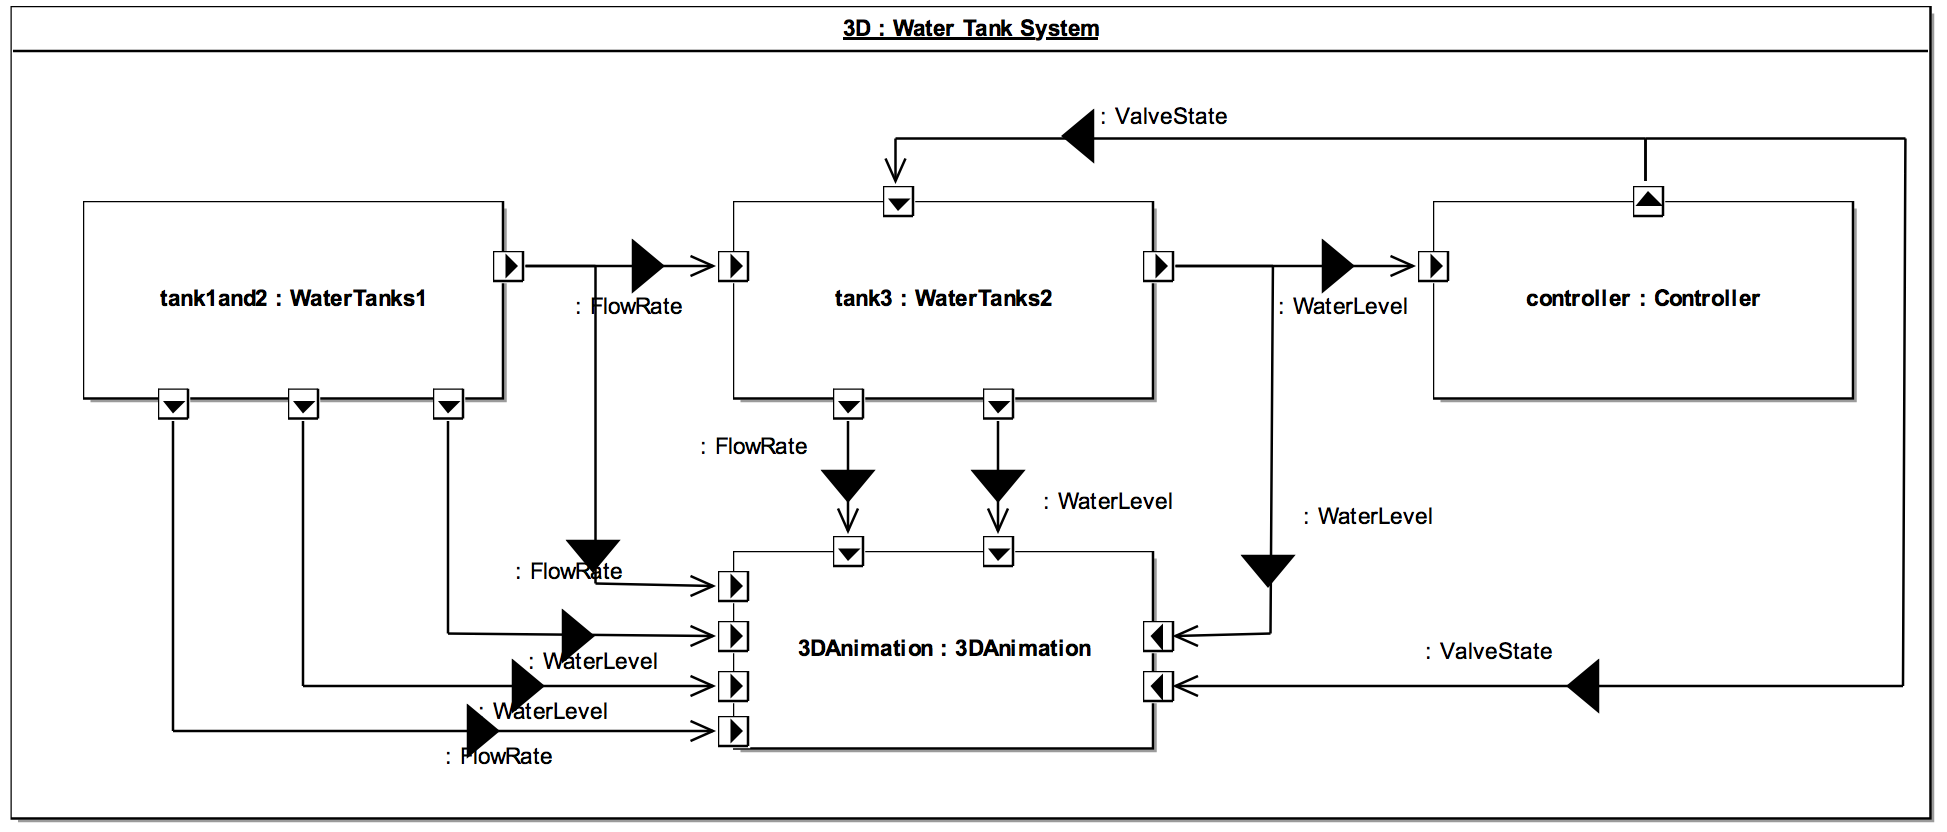
\includegraphics[width=0.85\textwidth]{threetank/ttwt_cd_vis.png}
\caption{Connections Diagram defining the Three-tank Water Tank system connections and elements for visualisation}
\label{fig:threetankcdvis}
\end{center}
\end{figure}

\subsection{Multi-model}
\label{sec:threetank_into_mm}

\subsubsection{Models}
\label{sec:threetank_into_models}

Given the ASD of the SysML model in  Section~\ref{sec:threetank_into_sys}, three (simulation) models are defined; two 20-sim subsystems and a VDM subsystem as shown in Figure~\ref{fig:threetankmm_ss}.

\begin{description}
\item[WaterTanks1, WaterTanks2] The partitioning of the 20-sim model is straightforward, with a single signal between the two 20-sim subsystems representing the flow of water between tanks 2 and 3. The rationale behind this split is that the flow rate between tank 1 and 2 has a high frequency and amplitude, suggesting that splitting the two tanks would result in erroneous results when time steps are imposed in co-simulation. 

\begin{figure}[htb!]
\begin{center}
\subfigure[Subsystems of Three-tank Water Tank multi-model]
{
     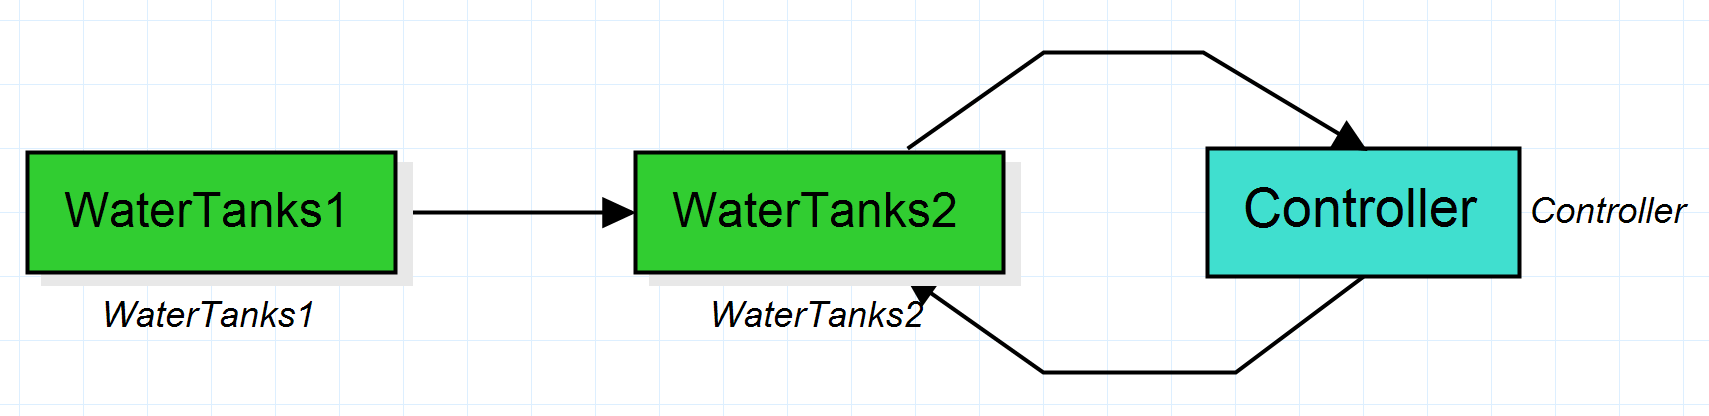
\includegraphics[width=0.6\linewidth]{threetank/ttwt_20sim_fmus} 
      \label{fig:threetankmm_ss}
}
\subfigure[WaterTanks1 subsystem]
{
     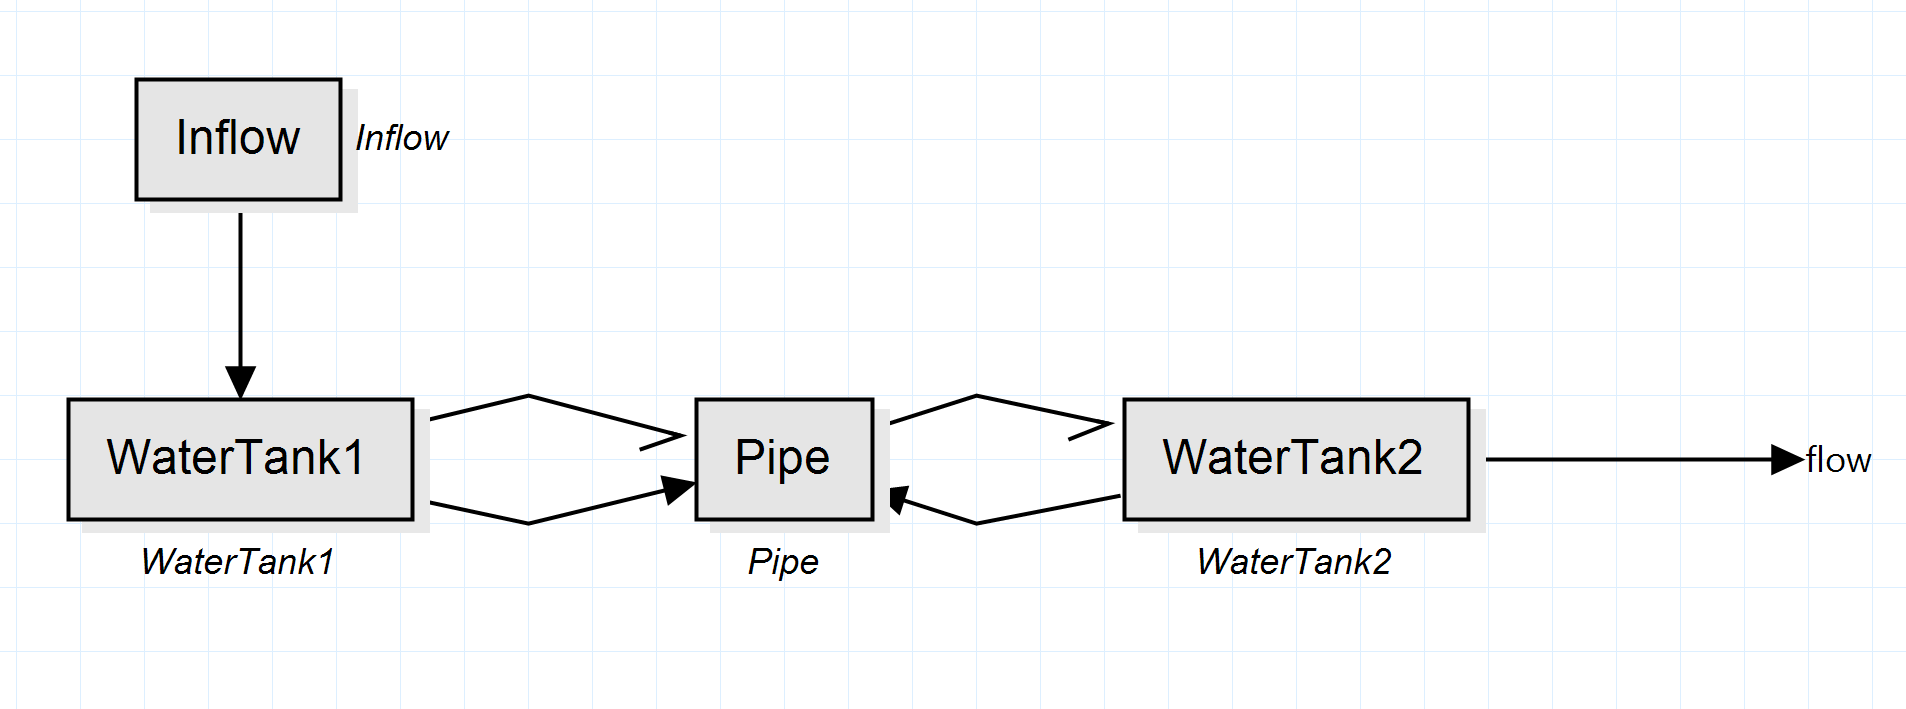
\includegraphics[width=0.6\linewidth]{threetank/ttwt_20sim_wt1fmu} 
      \label{fig:threetankmm_ss1}
}
\subfigure[WaterTanks2 subsystem]
{
     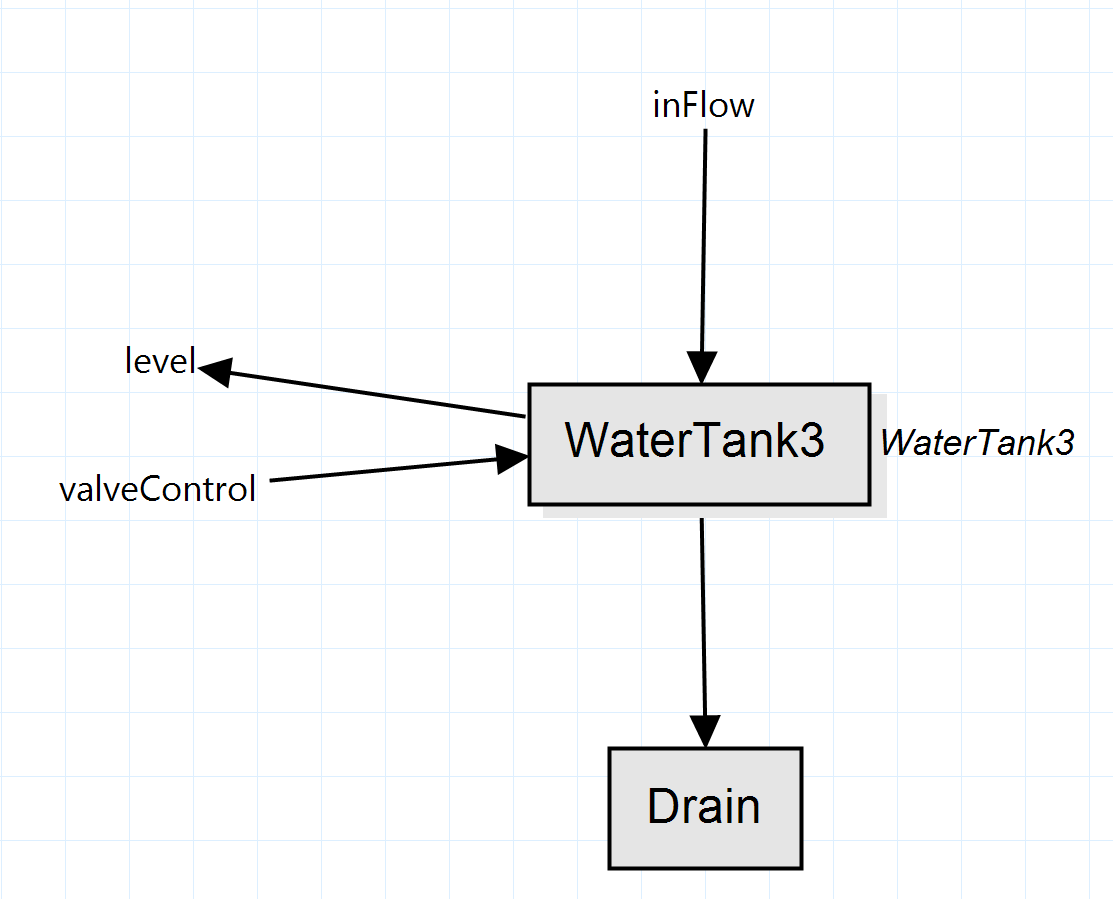
\includegraphics[width=0.35\linewidth]{threetank/ttwt_20sim_wt2fmu} 
      \label{fig:threetankmm_ss2}
}
\caption{20-sim models for the Three-tank Water Tank multi-model}
\label{fig:threetank_mm_20-sim}
\end{center}
\end{figure}

\item[Controller] The VDM-RT controller model is a simple controller, which governs \emph{Tank3}. The VDM-RT model contains a \emph{System} class containing \emph{HardwareInterface}  and \emph{Controller} objects -- \emph{hwi}  and \emph{controller}, respectively. The \emph{hwi} object includes the input and output variables of the model and design parameters. The \emph{controller} object is supplied with an instance of the \emph{LevelSensor}  (\emph{sensor}) and \emph{ValveActuator} (\emph{valve}) classes -- each given access to different parts of the \emph{hwi} object. The \emph{sensor} object represents the sensor that measures the current water level, and \emph{valve} is  represents the valve at the bottom of the tank.

The control loop retrieves the current level of water from the sensor and determines whether to set the valve to be open or closed depending on the level compared to some set maximum or minimum value. 
\end{description}

\subsubsection{Configuration}
\label{sec:threetank_into_mm}

Two multi-models are defined for the Three Tank Study corresponding to the two System block instances defined in the CDs of the SysML model in Section~\ref{sec:threetank_into_sys}. 

In the first multi-model (\emph{Non-3D}), there are three FMUs and three connections. The FMUs comprise: WaterTankController, threewatertank1 and threewatertank2 -- exported from the VDM-RT and 20-sim models described above. The connections are as follows: firstly between the \texttt{flow} port of \emph{WaterTanks1} to the \texttt{inFlow} of \emph{WaterTanks2}; secondly between \texttt{valveControl} port of the \emph{WaterTanks2} model to the \texttt{wt3\_valve} of the \emph{Controller}; and finally from the \texttt{wt3\_level} of the \emph{Controller} to the \texttt{level} port of \emph{WaterTanks2}. 

In addition, there are two \emph{design parameters} -- \texttt{wt3\_min} and \texttt{wt3\_max}, both of type \texttt{real}.

The complete configuration is given in Figure~\ref{fig:threetankconfig}.

\begin{figure}[htbp]
\begin{center}
\begin{config}
{		
	"fmus":{
		"{c}":"WaterTankController.fmu",
		"{t1}":"threewatertank1.fmu",
		"{t2}":"threewatertank2.fmu"
	},
	"connections":{
		"{c}.controller.wt3_valve":["{t2}.tank2.valveControl"],
		"{t1}.tank1.Tank2OutFlow":["{t2}.tank2.inFlow"],
		"{t2}.tank2.level":["{c}.controller.wt3_level"]
	},
	"parameters":{
		"{c}.controller.wt3_max":1.7,
		"{c}.controller.wt3_min":1.3
	}
}
\end{config}
\caption{Configuration file for Three-tank Water Tank system}
\label{fig:threetankconfig}
\end{center}
\end{figure}


The second multi-model (\emph{3D}) uses the 3D visualisation FMU, and has additional connections to that FMU, as shown in Figure~\ref{fig:threetankconfig2}.

\begin{figure}[htbp]
\begin{center}
\begin{config}
{
	"fmus":{
		"{c}":"WaterTankController.fmu",
		"{t1}":"threewatertank1.fmu",
		"{t2}":"threewatertank2.fmu",
		"{3d}":"3DAnimationFMU.fmu"
	},
	"connections":{
		"{c}.controller.wt3_valve":["{t2}.tank2.valveControl","{3d}.3DAnimationFMU.animation.tank3.valve.control"],
		"{t1}.tank1.Tank2OutFlow":["{t2}.tank2.inFlow","{3d}.3DAnimationFMU.animation.tank2.outflow"],
		"{t2}.tank2.level":["{c}.controller.wt3_level", "{3d}.3DAnimationFMU.animation.tank3.waterlevel"],
		"{t1}.tank1.Tank1InFlow":["{3d}.3DAnimationFMU.animation.tank1.inflow"],
		"{t1}.tank1.Tank1WaterLevel":["{3d}.3DAnimationFMU.animation.tank1.waterlevel"],
		"{t1}.tank1.Tank2WaterLevel":["{3d}.3DAnimationFMU.animation.tank2.waterlevel"],
		"{t2}.tank2.Tank3OutFlow":["{3d}.3DAnimationFMU.animation.tank3.outflow"],
		"{t2}.tank2.puddle":["{3d}.3DAnimationFMU.animation.drain.puddle"]
	},
	"parameters":{
		"{c}.controller.wt3_max":1.7,
		"{c}.controller.wt3_min":1.3
	}
}
\end{config}
\caption{Configuration file for Three-tank Water Tank system}
\label{fig:threetankconfig2}
\end{center}
\end{figure}

\subsection{Co-simulation}
\label{sec:threetank_into_co}

Using the INTO-CPS Co-simulation Engine (COE), we may simulate the three FMU multi-model. We are able to log the water level of tank 3 and the flow rate between tank 2 and 3. These values are shown in the graph in Figure~\ref{fig:threetankcoeres}, using a fixed step size of \emph{0.05}. A simulation time of at least 20 seconds is recommended so to observe changes in controller behaviour.

\begin{figure}[htbp]
\begin{center}
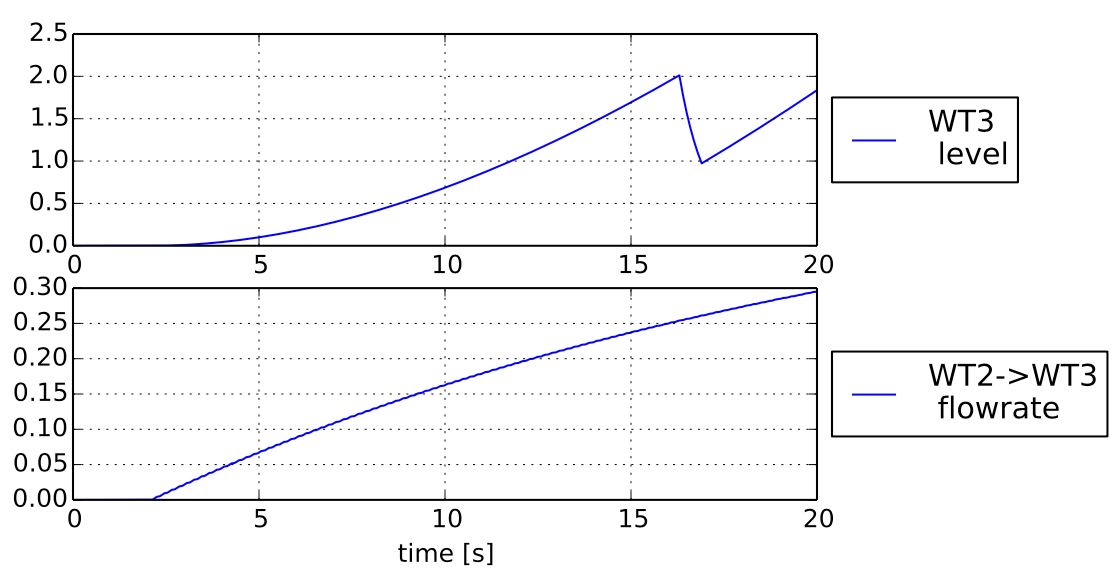
\includegraphics[width=0.85\textwidth]{threetank/ttwt_coe_res.png}
\caption{Simulation results using the INTO-CPS COE}
\label{fig:threetankcoeres}
\end{center}
\end{figure}

The results in the graph correspond closely to those of the baseline Crescendo model illustrated in~\cite{INTOCPSD3.4}. During simulation, the water level raised to the maximum value (2.0 meters) and at 16.3 seconds the tank 3 valve is opened by the VDM-RT controller and the level drops to just below the minimum (1.0 meters) and at 16.9 seconds the valve is closed and the water level begins to rise again.

Co-simulating the 3D multi-model opens a 3D visualisation window as shown in Figure~\ref{fig:threetank3d} which depicts the state of the Three-tank system as the simulation progresses. 

\begin{figure}[htbp]
\begin{center}
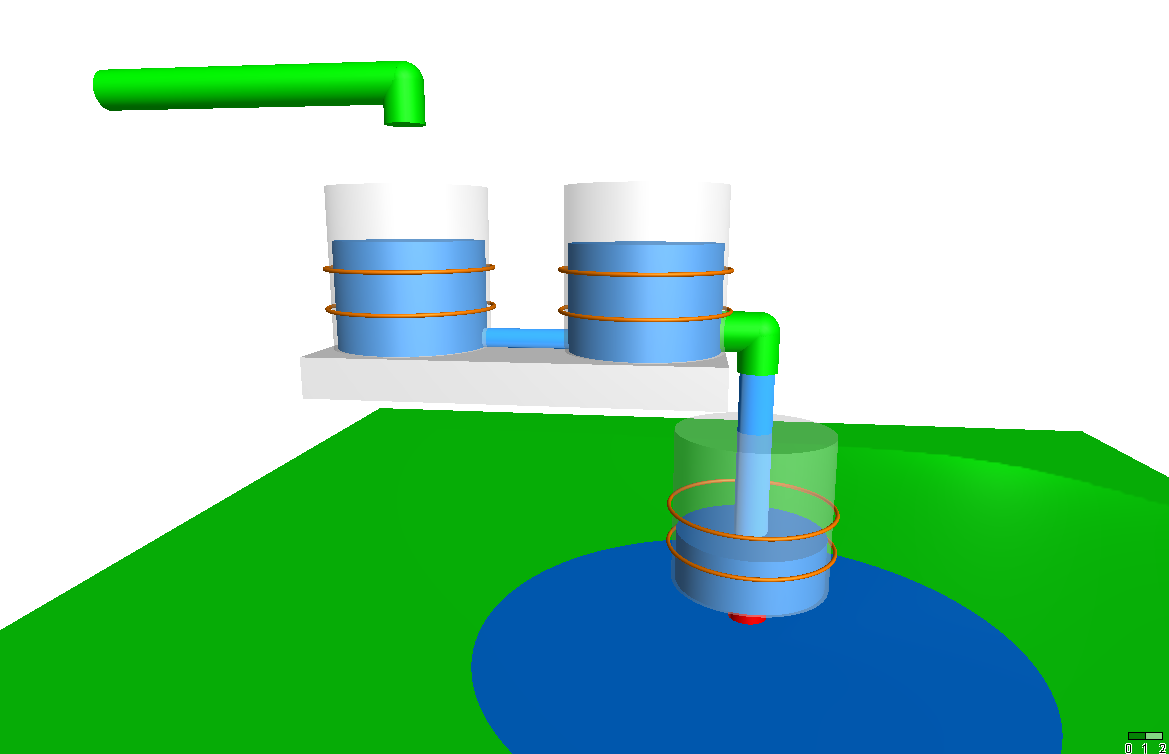
\includegraphics[width=0.75\textwidth]{threetank/TTWT_3D.png}
\caption{3D visualisation of the Three-tank Water Tank system}
\label{fig:threetank3d}
\end{center}
\end{figure}

\subsection{Analyses and Experiments}

\subsubsection{Design Space Exploration}
\label{sec:threetank_dse}

A simple DSE experiment is included in the project, which demonstrates the use of the DSE tool support. The experiment varies the two design parameters of the study -- \texttt{wt3\_min} and \texttt{wt3\_max}. These parameter values may be set between $0.2$ and $2.0$ in intervals of $0.2$. A constraint on the parameters (\texttt{{controller}.controller.wt3\_max $>$ {controller}.controller.wt3\_min}) ensures that the maximum water value is always larger than the minimum water level. 

Two objectives are defined: \textit{cumulativeDeviation} and \textit{vCount}. The first objective, \textit{cumulativeDeviation}, is to minimise the cumulative deviation from a desired level - set to $1.0$. The second objective, \textit{vCount}, is to minimise the number of valve operations -- i.e. have a lower number of valve state changes. The use of Pareto ranking, minimising both objectives gives the resultant graph in Figure~\ref{fig:threetankdse}.

\begin{figure}[h]
\begin{center}
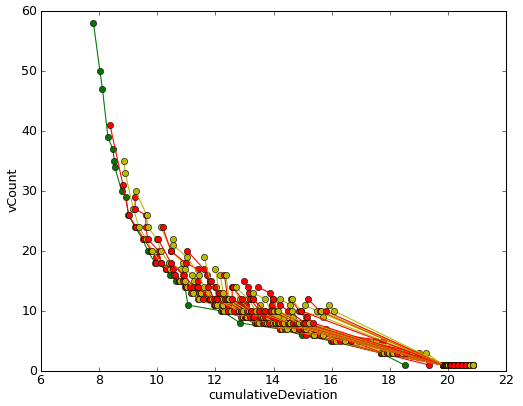
\includegraphics[width=0.75\textwidth]{threetank/dse_pareto_graph.png}
\caption{Design Space Exploration Pareto graph of the Three-tank Water Tank system}
\label{fig:threetankdse}
\end{center}
\end{figure}

From the results we see that there is a clear tradeoff to be made between levels which optimise  each objective -- it is for the engineer to determine which of these is more important. The green line on the graph (the left-most set of results) gives this `non-dominated' set of results -- also given as a table as in Figure~\ref{fig:threetankdsetable}. In broad terms the ranking shows: levels closer to the desired level (e.g. \texttt{wt3\_min} = $1.0$ and \texttt{wt3\_max} = $1.05$) produce results with a lower cumulative deviation, but higher valve operation count; and a minimum level further from the desired level (e.g. \texttt{wt3\_min} = $0.2$) produces results with a lower valve operation count, but higher cumulative deviation.

\begin{figure}[h]
\begin{center}
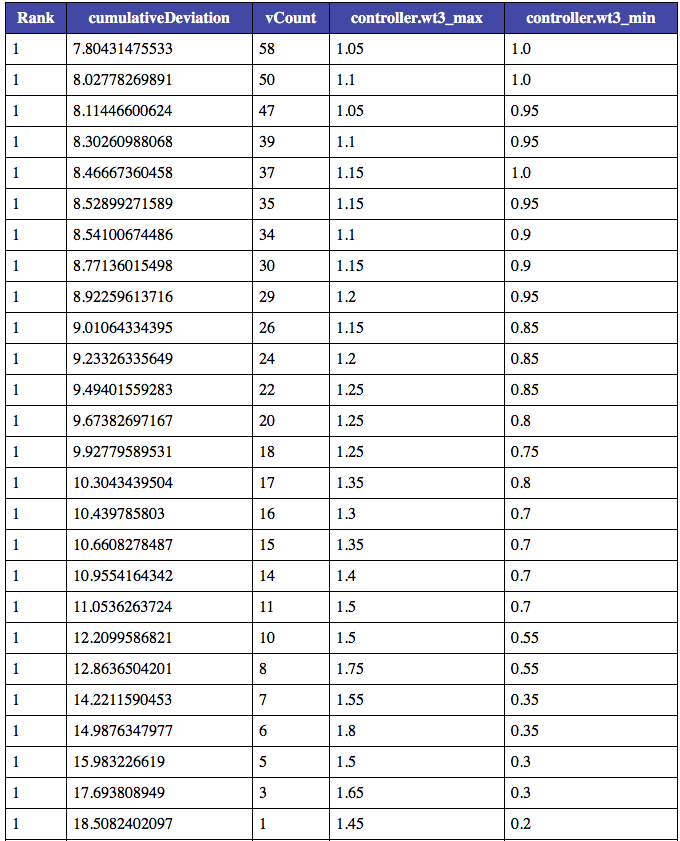
\includegraphics[width=0.75\textwidth]{threetank/dse_results_table_nds.png}
\caption{Design Space Exploration Pareto front table of the Three-tank Water Tank system}
\label{fig:threetankdsetable}
\end{center}
\end{figure}


\subsubsection{Test Automation}
\label{sec:threetank_ta}

\begin{figure}
\begin{center}  
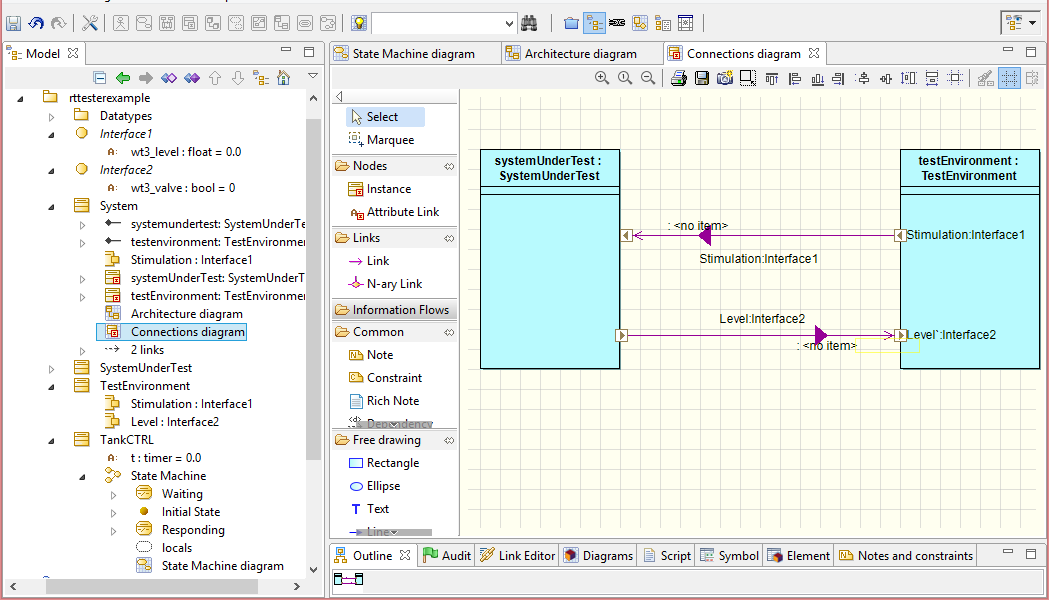
\includegraphics[width=\textwidth]{threetank/ta_overview}
\caption{Overview of the three-tank test model in Modelio}
\label{fig:threetanktestmodel}
\end{center}
\end{figure}

Test automation can also be applied to the controller of the three-tank example. A SysML model exists that
represents the test model for this system which can be used to produce tests for models and implementations of the
controller in RT-Tester\footnote{Note that this is a different SysML model used for the co-simulation multi-model.}. The model consists of a specified System Under Test (SUT), which in this case corresponds to
the controller, and the Test Environment (TE) which is the rest of the water tank system, but specifically the water
tank the controller is monitoring. A screen shot giving an overview of the test model is shown in
Figure~\ref{fig:threetanktestmodel}.

The  SUT and TE are specified using the blocks \emph{SystemUnderTest} and \emph{TestEnvironment}, respectively. The SUT
block an input flow port called \emph{Stimulation} of type \emph{Interface1} and an output port of type
\emph{Interface2}. The TE has the same ports but in the opposite direction. \emph{Interface1} specifies the shared
variables that the SUT will read from. In this case it consists of a single variable \emph{wt3\_level}, as seen on the
right, which corresponds to the FMU input. Likewise, \emph{Interface2} specifies the shared variable that the SUT will
write to, in this case the variable \emph{wt3\_valve} which gives the valve status. The two blocks are linked together
so that the SUT and TE can communicate on these channels.

\begin{figure}
\begin{center}  
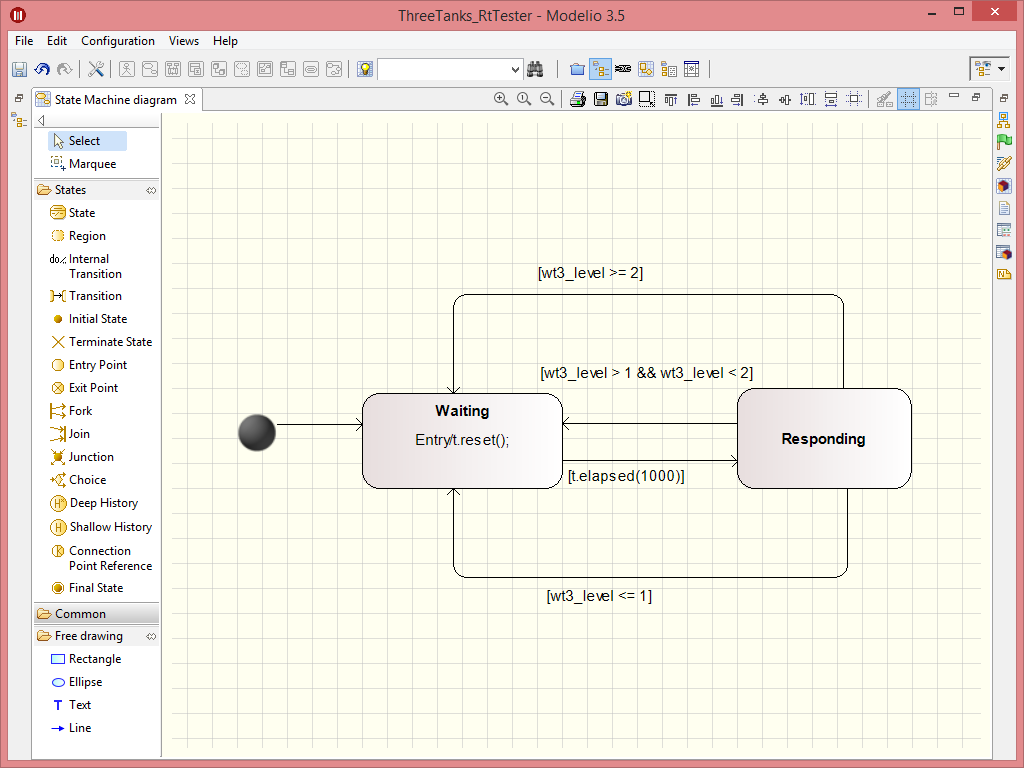
\includegraphics[width=\textwidth]{threetank/ta_state_machine}
\caption{State machine for abstract behaviour of three-tank controller}
\label{fig:threetankstatemachine}
\end{center}
\end{figure}

In order to generate tests it is necessary to specify an abstract model for the controllers behaviour, which should be
modelled using a timed state machine. We thus created the SysML state machine diagram shown in
Figure~\ref{fig:threetankstatemachine}. The three-tanks controller is relatively simple and so the state machine has
only two states. The \textbf{Waiting} state means that the controller is waiting until sufficient time has elapsed to
poll the sensors and act accordingly. It has a single outgoing transition with the guard \texttt{t.elapsed(1000)}. The
variable \texttt{t} is a timer for this state machine. It advances in time and can be checked and reset at certain
points, rather like a stop-watch. The state machine changes to the \textbf{Responding} state once 1000 ms (1 s) has
elapsed.

The \textbf{Responding} state contains the main decision logic for the controller. It has three outgoing edges with
guards and actions (the latter are not shown). If the water level polled on variable \emph{wt3\_level} remains within
the safe zone of between 1 and 2 then the state machine returns to state \textbf{Responding} with no action. If the
water level is greater than or equal to 2, the \emph{wt3\_valve} variable is set to 0 to shut off the valve, and the
controller returns to the \textbf{Waiting} state. Otherwise, if the level is less than or equal to 1, then the valve is
turned on by setting \emph{wt3\_valve} to 1.

\begin{figure}
  \begin{center}
    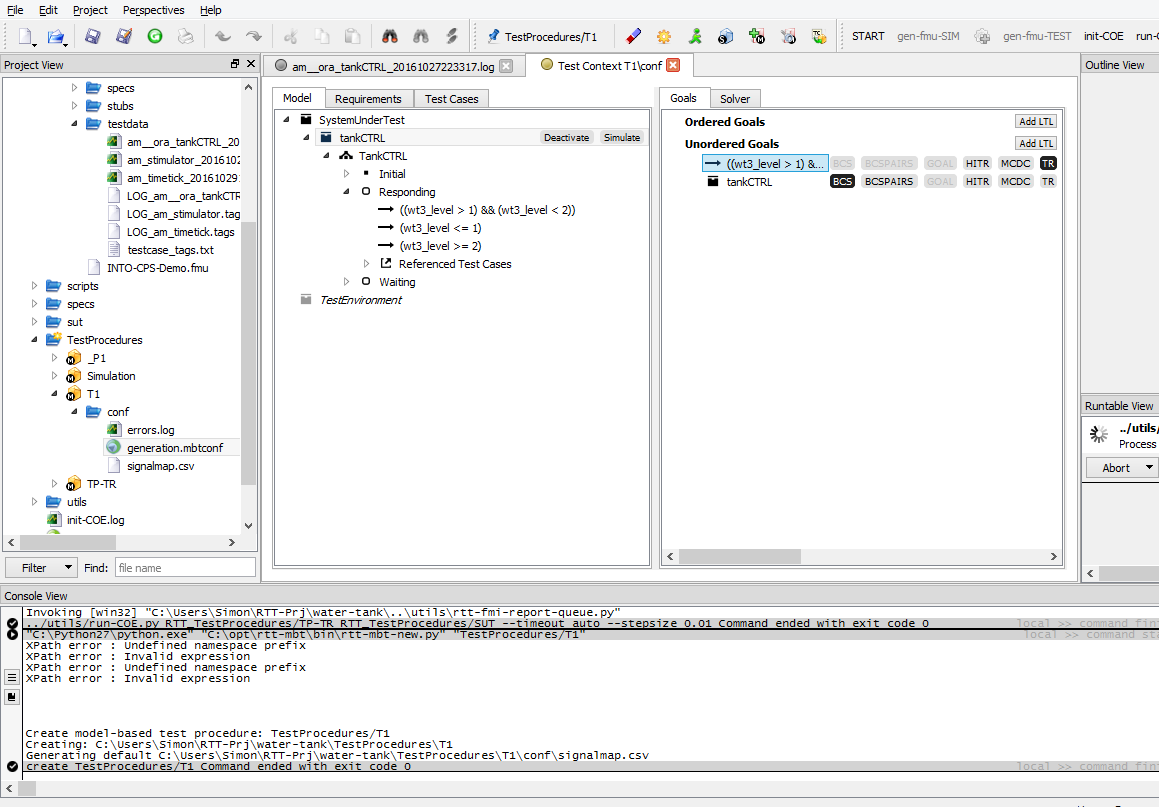
\includegraphics[width=16cm]{threetank/ta_rtt2.png}
  \end{center}
  \caption{Configuring a test procedure}
  \label{fig:ta-proc}
\end{figure}

This behavioural model must be input into RT-Tester to generate and execute tests. We do this by first exporting XMI from Modelio by
selecting the project name, and then the menu item \emph{Import / Export > Export > XMI export}. The model can then be
imported from RT-Tester by selecting \emph{Project > Model-based testing > Import model > Import from file}. This
currently must be done from the existing \emph{water-tanks} model available in RT-Tester to ensure that the FMU is
correctly set up. One of the standard test procedures can then be run, or a new test procedure can be created by
selecting \emph{New > MBT Test Procedure} and then using test procedure \texttt{TestProcedures/\_P1} as a
template. Suitable tests can be configured from the \emph{conf > generation.mbtconf} file in the new directory as
illustrated in Figure~\ref{fig:ta-proc}.

\begin{figure}
  \begin{center}
    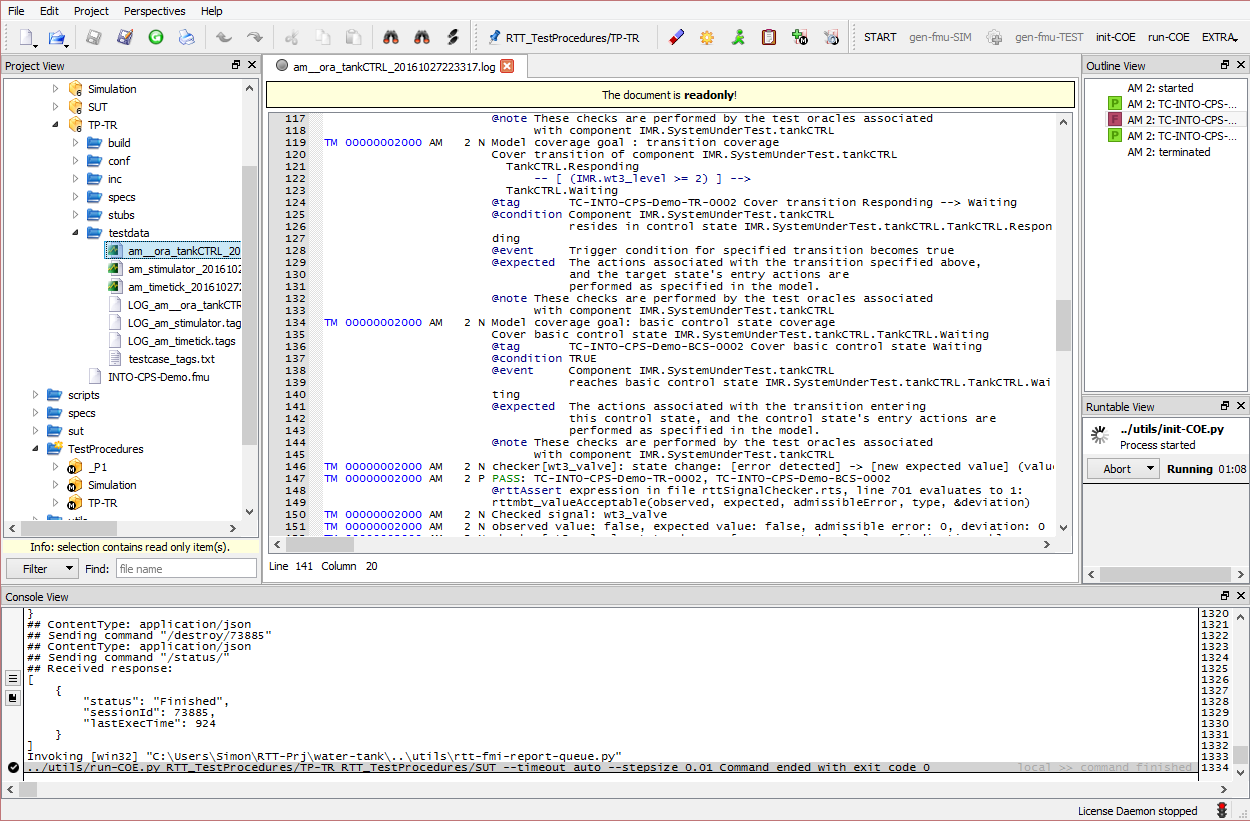
\includegraphics[width=16cm]{threetank/ta_rtt1.png}
  \end{center}
  \caption{Test procedure output}
  \label{fig:ta-out}
\end{figure}


The project can then be prepared for executing the tests through the \emph{init-Project} command that creates the test
FMUs. Finally, the test procedure can be executed by starting the COE, and then using the \emph{run-COE} command. This
will produce output which is exemplified in Figure~\ref{fig:ta-out}.

\subsubsection{Code Generation}

The VDM-RT model, \textbf{WaterTankController} can be exported from Overture as a C code FMU, in addition to the tool wrapper FMU as used above. The \emph{WaterTankController-SourceCode.FMU} included in this pilot is obtained directly from Overture using the ``Export Source Code FMU'' option. However, this FMU does not contain binaries for co-simulation and so one may use the \emph{FMU Builder} included in the INTO-CPS Application to compile FMUs for Windows, Mac and Linux. 

This process has been performed and the resultant FMU is included in the pilot in the FMUs folder; \emph{WaterTankController-Standalone.FMU}. One example experiment available is to switch this FMU for the tool wrapper version -- \emph{WaterTankController.FMU} -- and compare results. 
\clearpage
\graphicspath{ {fcu/} }

\section{Fan Coil Unit}

\subsection{Test Model}
The test model is developed based on the model of the FCU controller in VDMRT. Basically, it is a PID controller.

\subsubsection{Inputs and Outputs}
The SystemUdnerTest receives the following inputs (stimuli) from the TestEnvironment:
\begin{itemize}
    \item $RAT$: set point of room air temperature 
    \item $RATSP$: current room air temperature 
\end{itemize}

The SystemUdnerTest provides the following observable outputs to the TestEnvironment:
\begin{itemize}
    \item $fanSpeed$: fan speed  
    \item $valveOpen$: valve open state 
\end{itemize}

\subsubsection{Constant Variables and Local Variables}
Several constant variables below are defined. The access model property of all these variables is defined as \B{Read}.  
\begin{itemize}
	\item $K$: proportional gain
	\item $N$: derivative gain limitation
	\item $Td$: derivative time constant 
	\item $Ti$: integral time constant 
	\item $b$: proportional setpoint weighting parameter
	\item $c$: derivative setpoint weighting parameter 
    \item $sampletime$: sample time 
\end{itemize}

Other local variables are used to store intermediate results. However their access model property is set to \B{Read/Write}.

\begin{figure}[htb!]
    \centering
    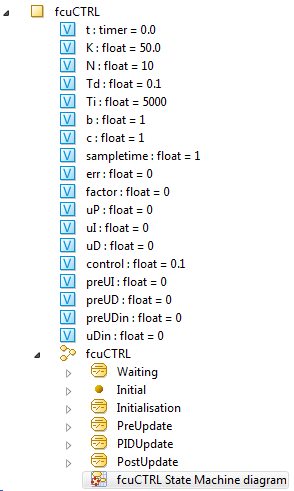
\includegraphics[width=0.4\textwidth]{fcu_sut_vars}
    \caption{Variables of LFR Controller}
    \label{fig:fcu-var}
\end{figure}


\subsubsection{State Machine Diagram}
When the state machine is residing in the \verb+Waiting+ state, it moves to processing states which are consisted of three states:
\begin{itemize}
    \item \verb+PreUpdate+: calculate numbers of local variables ($factor$, $err$, and $uDin$), that will be used in the next state, according to current inputs.
    \item \verb+PIDUpdate+: the transition of \verb+PreUpdate+ to this depends on the value of $RATSP$. If it is larger than 1, $uI$ will be updated. Otherwise, $uI$ is equal to 0. This is designed for anti integral windup.
    \item \verb+PostUpdate+: update $preUDin$, $preUI$ and $preUD$ that are used for sequential updates. 
\end{itemize}
Finally, the transition from \verb+PostUpdate+ to \verb+Waiting+ calculates (based on updated $uP$, $uI$ and $uD$) and outputs $fanSpeed$ and $valveOpen$ to its environment.

\begin{figure}[htb!]
    \centering
    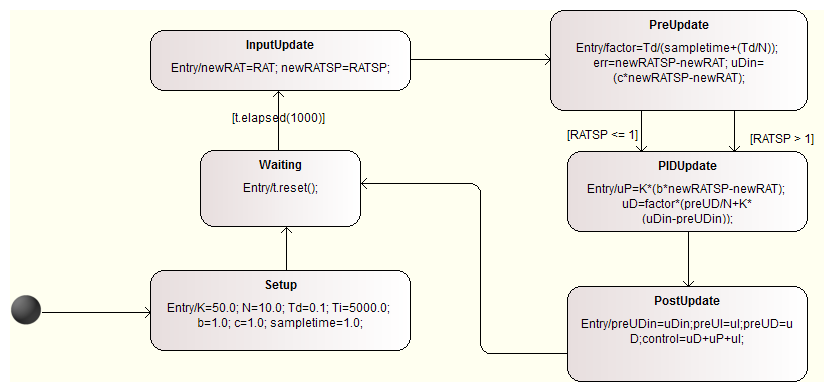
\includegraphics[width=1.0\textwidth]{fcu_sut_sm}
    \caption{State Machine Diagram of SUT}
    \label{fig:fcu-sut-sm}
\end{figure}

It is worth noting that
\begin{itemize}
    \item additional state \verb+Setup+ is used to set up all constants,
\end{itemize}

\subsection{A Manual Implementation of SUT in C}

The source code is listed as follows.

\lstset{language=C,
    basicstyle=\footnotesize\ttfamily,
    keywordstyle=\color{blue}\ttfamily,
    stringstyle=\color{red}\ttfamily,
    commentstyle=\color{green}\ttfamily,
    morecomment=[l][\color{magenta}]{\#},
    tabsize=2
}

\begin{lstlisting}
#include <stdio.h>
#include <sys/time.h>
#include <sys/types.h>
#include "fcu_ctrl.h"

const float K = 50.0;
const float Td = 0.1;
const float N = 10;
const float Ti = 5000;
const float b = 1;
const float c = 1;
const float sampletime = 1;

float err = 0;
float factor = 0;
float uDin = 0;
float uP = 0;
float uD = 0;
float uI = 0;
float control = 0.1;
float MV = 0;
float totaluI = 0;
float preUI = 0;
float totaluDin = 0;
float preuDin = 0;

#define _ms( t ) ( (t) * 1000 )

VSTimer_t t;

void reset( VSTimer_t* timer)
{
	struct timeval now;
	ti_gettimeofday( &now, NULL );
	*timer = now.tv_sec * 1000000 + now.tv_usec;
}

BOOLEAN elapsed( VSTimer_t* timer, long usec )
{
	struct timeval now;
	long long usec_now;

	ti_gettimeofday( &now, NULL );
	usec_now = now.tv_sec * 1000000 + now.tv_usec;
	return ( ( usec_now - (*timer) ) >= usec );
}

/** Initialize SUT */
void sut_init()
{
	reset(&t);
}

/** Run SUT (one step) */
void sut_run(float RAT, float RATSP, 
    float* fanSpeed, float* valveSpeed)
{
	err = RATSP - RAT;
	factor = Td/(sampletime + (Td/N));
	uP = K*(b*RATSP - RAT);

	if (RATSP > 1)
	uI = preUI + sampletime * (K * err/Ti);
	else
	uI = 0;
	preUI = uI;

	uDin = c*RATSP-RAT;
	uD = factor * (uD/N + K *(uDin - preuDin));
	preuDin = uDin;

	control = uP + uI + uD;
	*fanSpeed = control;
	*valveSpeed = control;

	return;
}
\end{lstlisting}

\subsubsection{Build of the implementation and Setup of Execution context Test Procedure}
A python script \verb+build-sut.py+ is used to build the SUT implementation and create the test procedure SUT under \verb+RTT_TestProcedures+. The main part is illustrated below.

\lstset{language={},
    basicstyle=\footnotesize\ttfamily,
    showstringspaces=false,
    tabsize=2
}
\begin{lstlisting}
print("## -- Building SUT -----------------------------")
try:
  print("## -- Wrapping SUT to FMU --------------------")
  os.chdir(os.path.join(context, "sut"))
  print("## Compiling sample SUT implementation in '{0}'".
    format(os.getcwd()))
  if 0 != os.system(" ".join([PROG_make,"all"])):
    raise NameError("Make Failed!")
  print("## Creating RTT_TestProcedures/SUT as wrapper to the 
    modelDescription.xml that fits to SUT".format(os.getcwd()))
  os.chdir(context)
  if not py(" ".join([PROG_wrap, "--model-description", 
      os.path.join(context, "RTT_TestProcedures", "Simulation", 
        "model", "modelDescription.xml"), 
      "RTT_TestProcedures/SUT"])):
    raise NameError("Wrapping of SUT failed")
  print("## -- Modifying test procedure...")
  append_to_file("""
// -- Added for SUT inclusion -----
CFLAGS  ; -I$(RTT_TESTCONTEXT)/sut
INCLUDE ; fcu_ctrl.h
LDPATH  ; -L$(RTT_TESTCONTEXT)/sut 
LDFLAGS ; -lfcu_ctrl
// --------------------------------
""", os.path.join(context, "RTT_TestProcedures", "SUT", 
    "conf", "swi.conf"))
define_sut_in_rts("""
@abstract machine sut()
{					   
	@INIT:{			   
		fprintf(stderr, "CALL SUT INIT\\n");
		sut_init();						   
	}									   
	@FINIT:{							   
		//
	}
	@PROCESS:{
		float RATSP;
		float RAT;
		float valveOpen;
		float fanSpeed;

		fprintf(stderr, "STARTING SUT PROCESS\\n");

		while(@rttIsRunning){
			/* Map FMU input variables to SUT: X = rttIOPre->X */
			RATSP = rttIOPre->RATSP;
			RAT = rttIOPre->RAT;

			sut_run(RAT, RATSP, &fanSpeed, &valveOpen);

			/* Map SUT output to FMU output: rttIOPost->X = X */
			rttIOPost->fanSpeed = fanSpeed;
			rttIOPost->valveOpen = valveOpen;

			@rttWaitSilent(1 _ms);
		}
	}
}
int ti_gettimeofday(struct timeval *tv, struct timezone *tz){
	tv->tv_sec	= @t / 1000;		  
	tv->tv_usec = (@t % 1000) * 1000;
	return 0; 
}
""", os.path.join(context, "RTT_TestProcedures", 
  "SUT", "specs", "fmi2sut.rts"))
\end{lstlisting}

\subsubsection{Project Actions}
An action named \verb+sut_build+ is added in the test project to build the SUT implementation and SUT test procedure automatically. The definition of its command is
\begin{verbatim}
c:/python27/python.exe <PROJECT-LOCAL-PATH>/sut/build-sut.py
\end{verbatim}

\subsection{Test Automation}

Not all test cases for BCS and TR are passed when running against simulation or SUT when latency of outputs is set to either 100ms or 10ms. Failures occur at time stamp 2101.
\lstset{language={},
    basicstyle=\scriptsize\ttfamily,
    showstringspaces=false,
    tabsize=2
}
\begin{lstlisting}
TM 00000002000 AM   2 N checker[fanSpeed]: state change: [indication ok] -> 
                        [new expected value] (value: 93.750495910644531)
TM 00000002000 AM   2 N checker[valveOpen]: state change: [indication ok] -> 
                        [new expected value] (value: 93.750495910644531)
TM 00000002101 AM   2 E FAIL (1) : TC-INTO-CPS-Demo-BCS-0006, TC-INTO-CPS-Demo-BCS-0002
                        @rttAssert expression in file rttSignalChecker.rts, line 701 evaluates to 0:
                        rttmbt_valueAcceptable(observed, expected, admissibleError, type, &deviation)
TM 00000002101 AM   2 N Checked signal: fanSpeed
TM 00000002101 AM   2 N observed value: 0, expected value: 93.750495910644531, 
                      admissible error: 9.9999999999999995e-008, deviation: 93.750495910644531
TM 00000002101 AM   2 N Failure description: latency elapsed for expected SUT output change.
TM 00000002101 AM   2 N checker[fanSpeed]: state change: [new expected value] -> [error detected]
TM 00000002101 AM   2 E FAIL (2) : TC-INTO-CPS-Demo-BCS-0006, TC-INTO-CPS-Demo-BCS-0002
                        @rttAssert expression in file rttSignalChecker.rts, line 701 evaluates to 0:
                        rttmbt_valueAcceptable(observed, expected, admissibleError, type, &deviation)
TM 00000002101 AM   2 N Checked signal: valveOpen
TM 00000002101 AM   2 N observed value: 0, expected value: 93.750495910644531, 
                        admissible error: 9.9999999999999995e-008, deviation: 93.750495910644531
TM 00000002101 AM   2 N Failure description: latency elapsed for expected SUT output change.
TM 00000002101 AM   2 N checker[valveOpen]: state change: [new expected value] -> [error detected]
\end{lstlisting}

However all are passed when the latency of outputs is set to 1000ms though there are two warnings. But the latency should be wrong.

\begin{lstlisting}
TM 00000003000 AM   2 W WARNING (1) : A new expected value 0 for signal fanSpeed did 
                        occur while still checking the last expected value 93.750495910644531
                        @rttCheck expression in file rttSignalChecker.rts, line 628 evaluates to 0:
                        current_state != rttmbt_new_expected
TM 00000003000 AM   2 P PASS: TC-INTO-CPS-Demo-BCS-0006, TC-INTO-CPS-Demo-BCS-0002
                        @rttAssert expression in file rttSignalChecker.rts, line 701 evaluates to 1:
                        rttmbt_valueAcceptable(observed, expected, admissibleError, type, &deviation)
TM 00000003000 AM   2 N Checked signal: fanSpeed
TM 00000003000 AM   2 N observed value: 0, expected value: 0, admissible error: 9.9999999999999995e-008, deviation: 0
TM 00000003000 AM   2 N checker[fanSpeed]: state change: [new expected value] -> [indication ok]
TM 00000003000 AM   2 W WARNING (2) : A new expected value 0 for signal valveOpen did 
                        occur while still checking the last expected value 93.750495910644531
                        @rttCheck expression in file rttSignalChecker.rts, line 628 evaluates to 0:
                        current_state != rttmbt_new_expected
TM 00000003000 AM   2 P PASS: TC-INTO-CPS-Demo-BCS-0006, TC-INTO-CPS-Demo-BCS-0002
                        @rttAssert expression in file rttSignalChecker.rts, line 701 evaluates to 1:
                        rttmbt_valueAcceptable(observed, expected, admissibleError, type, &deviation)
TM 00000003000 AM   2 N Checked signal: valveOpen
\end{lstlisting}

Some important points:
\begin{itemize}
    \item previously, do-action is used to initialise constants in the states \verb+Setup+. However, it seems that it has not executed. The operational semantics of do-actions is given in~\cite{VSI-mbt-man}: \I{if no state machine transition is enabled, the active simple state’s do-action and those of its ancestors are executed}. Eventually, since \verb+Setup+ is not a stable state, it will change to \verb+Waiting+ immediately and its do-action is not executed.
    \item it is necessary to change admissible errors of signal map, such as 0.0000001.
    \item TODO: find out the cause of failures for Simulation or SUT.
\end{itemize}

\subsection{Model Checking}
\begin{description}
    \item[P1] Constants will not be changed. 
\begin{verbatim}
Finally ([IMR.SystemUnderTest.fcuCTRL.fcuCTRL.Setup] and 
  Next (Globally ( [
    IMR.SystemUnderTest.fcuCTRL.K == 50.0 && 
    IMR.SystemUnderTest.fcuCTRL.N == 10.0 && 
    IMR.SystemUnderTest.fcuCTRL.Td == 0.1 && 
    IMR.SystemUnderTest.fcuCTRL.Ti == 5000 && 
    IMR.SystemUnderTest.fcuCTRL.b == 1 && 
    IMR.SystemUnderTest.fcuCTRL.c == 1 && 
    IMR.SystemUnderTest.fcuCTRL.sampletime == 1
])))
\end{verbatim}
    \item[P2] $fanSpeed$ of (RATSP=20, RAT=10) is larger than that of (RATSP=20, RAT=15)
    \item[P3] $RAT$ will approach $RATSP$  (how to simulate environment?)
\end{description}


\section{Fan Coil Unit (With Room and Wall)}
\subsection{Test Model}
The developed test model includes the FCU controller, the Room and Wall models. We use the Euler method to model continuous parts Wall and Room. 

\subsubsection{Inputs and Outputs}
The SystemUdnerTest receives the following inputs (stimuli) from the TestEnvironment:
\begin{itemize}
    \item $OAT$: outside air temperature 
    \item $RATSP$: room air temperature set point
\end{itemize}

The SystemUdnerTest provides the following observable outputs to the TestEnvironment:
\begin{itemize}
    \item $RAT\_out$: room air temperature 
\end{itemize}

\subsubsection{SystemUnderTest}
The SystemUnderTest consists of a FCU controller, a wall model and a room model.

The architecture diagram of SystemUnderTest is shown in Figure~\ref{fig:fcu_sut_sad}. 
\begin{figure}[htb!]
    \centering
	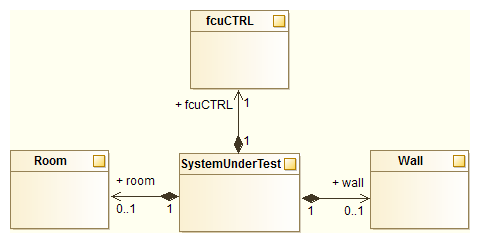
\includegraphics[width=0.8\textwidth]{roomwall/fcu_sut_sad}
    \caption{Architecture Diagram of SUT}
    \label{fig:fcu_sut_sad}
\end{figure}

\subsubsection{FCU Controller}
\paragraph{Inputs and Outputs}
The fcuCTRL receives the following inputs (stimuli):
\begin{itemize}
    \item $RAT\_out$: room air temperature from Room
    \item $RATSP$: room air temperature set point from TestEnvironment
\end{itemize}

The fcuCTRL provides the following outputs to the Room:
\begin{itemize}
    \item $fanSpeed$: fan speed 
    \item $valveOpen$: valve open state
\end{itemize}

The state machine diagram of fcuCTRL is illustrated in Figure~\ref{fig:fcu_sut_fcuctrl_sm}.
\begin{figure}[htb!]
    \centering
	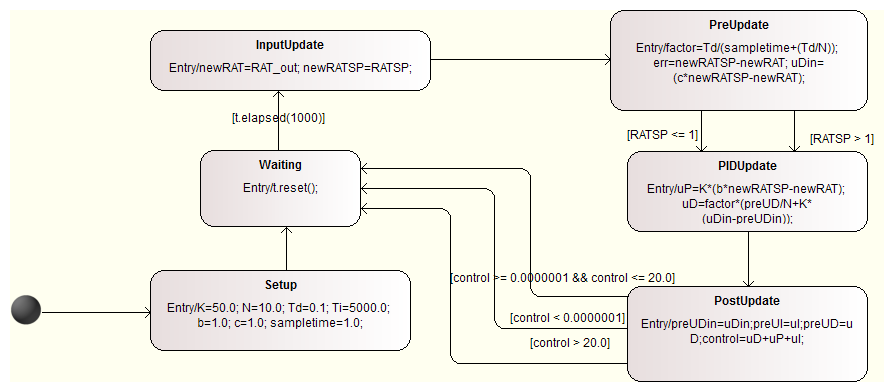
\includegraphics[width=1.0\textwidth]{roomwall/fcu_sut_fcuctrl_sm}
    \caption{State Machine Diagram of fcuCTRL}
    \label{fig:fcu_sut_fcuctrl_sm}
\end{figure}

\begin{itemize}
    \item \verb+Setup+ is used to initialize constant variables,
    \item After, the state machine resides in the \verb+Waiting+ state most of the time,
    \item After every one second, it starts to calculate PID parameters again,
        \begin{itemize}
            \item At first, update inputs $RAT$ and $RATSP$,
            \item Then calculate $uP$, $uD$, $uI$, and update other local variables for future use,
            \item Next calculate summation of $uP$, $uD$, and $uI$ to get $control$,
            \item Finally, limit $control$ and assign it to $fanSpeed$ and $valveSpeed$.
        \end{itemize}
\end{itemize}

\subsubsection{Wall}
\paragraph{Inputs and Outputs}
Wall receives the following inputs (stimuli):
\begin{itemize}
    \item $RAT\_out$: room air temperature from Room 
    \item $OAT$: outside air temperature from TestEnvironment 
\end{itemize}

Wall provides the following outputs to Room:
\begin{itemize}
	\item $Tisurf$: wall internal surface temperature
\end{itemize}

The state machine diagram of Wall is illustrated in Figure~\ref{fig:fcu_sut_wall_sm}.
\begin{figure}[htb!]
    \centering
	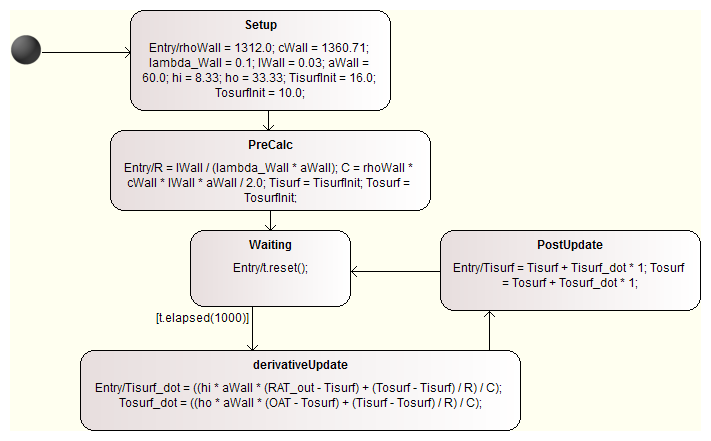
\includegraphics[width=1.0\textwidth]{roomwall/fcu_sut_wall_sm}
    \caption{State Machine Diagram of Wall}
    \label{fig:fcu_sut_wall_sm}
\end{figure}

\subsubsection{Room}
\paragraph{Inputs and Outputs}
Room receives the following inputs (stimuli):
\begin{itemize}
    \item $fanSpeed$: fan speed from fcuCTRL
    \item $valveOpen$: valve open state from fcuCTRL
	\item $Tisurf$: wall internal surface temperature from Wall
\end{itemize}

Room provides the following outputs to fcuCTRL and TestEnvironment:
\begin{itemize}
    \item $RAT\_out$: room air temperature
\end{itemize}

The state machine diagram of Room is illustrated in Figure~\ref{fig:fcu_sut_room_sm}.
\begin{figure}[htb!]
    \centering
	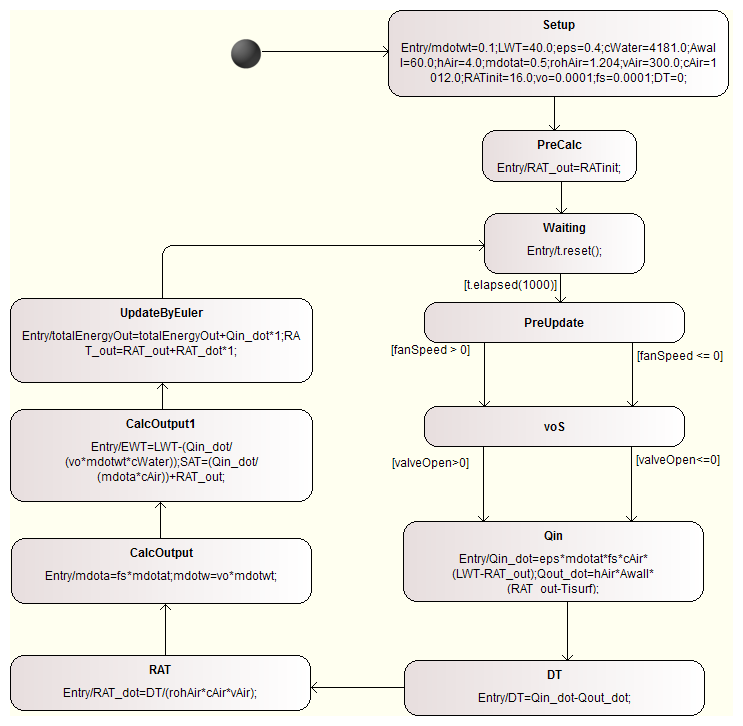
\includegraphics[width=1.0\textwidth]{roomwall/fcu_sut_room_sm}
    \caption{State Machine Diagram of Room}
    \label{fig:fcu_sut_room_sm}
\end{figure}

\subsection{Manual Implementations of SUT in C}
Two SUTs are implemented manually,
\begin{itemize}
    \item one standalone SUT to implement fcuCTRL, Room and Wall in C (correspond to SystemUnderTest in the test model),
    \item another SUT to implement fcuCTRL only in C, and then use the RoomHeating FMU from either 20-Sim or Modelica for Room and Wall.
\end{itemize}

\subsection{Test Automation}
\subsubsection{Test Input Sequence}
The inputs to FCU, $OAT$ and $RATSP$, is simulated through a state machine diagram in TestEnvironment. They are shown as $SUT\_OAT$ and $SUT\_RATSP$ in Figure~\ref{fig:fcu_co-sim-result}. $OAT$ changes slightly but $RATSP$ vibrates between 10 and 35 degrees.

\subsubsection{Test Run Configurations}
Three test configurations are provided for test automation with COE.
\begin{description}
    \item[SIM] TP against Simulation (Simulation is a SUT created from the test model), 
    \item[SUT] TP against the standalone SUT, 
    \item[SUT\_RoomWall] TP against the fcuCTRL SUT and RoomHeating FMU (therefore three FMUs).
\end{description}

Their test results are displayed in Figure~\ref{fig:fcu_co-sim-result}.
\begin{figure}[htb!]
    \centering
	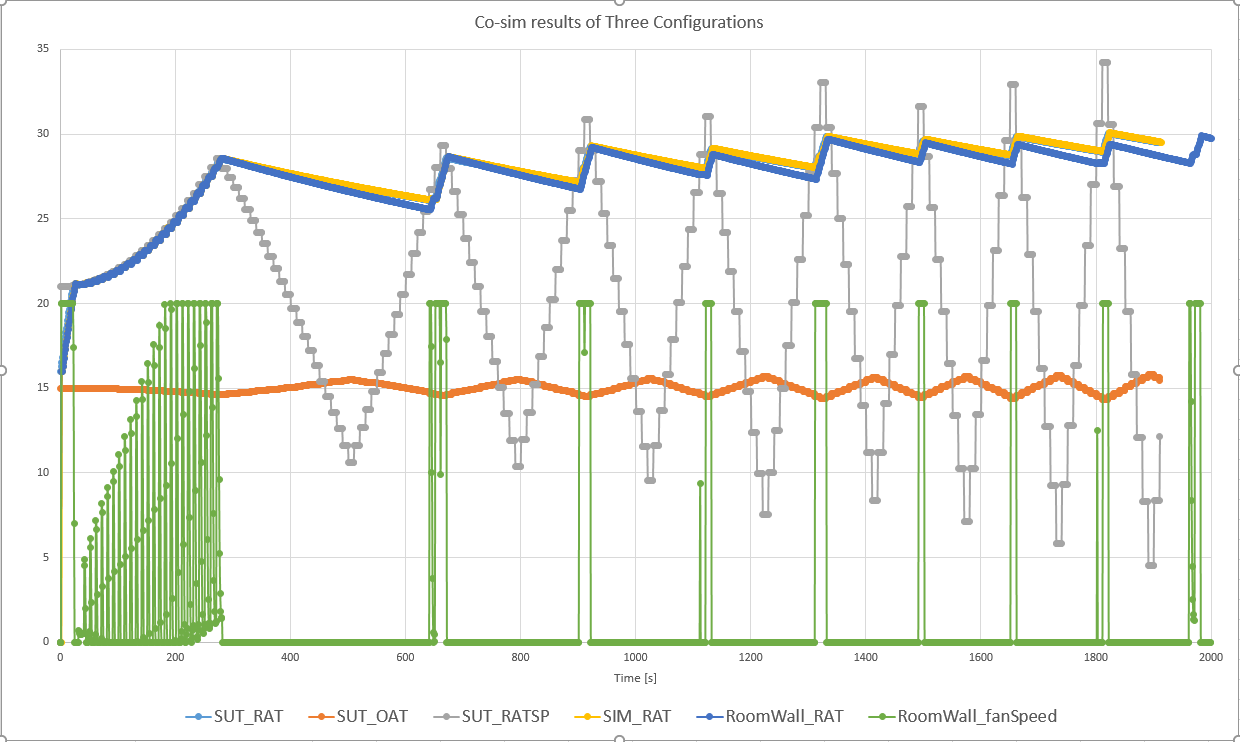
\includegraphics[width=1.0\textwidth]{test_results-20170621/fcu_co-sim-result}
    \caption{Test Results of Three Configurations}
    \label{fig:fcu_co-sim-result}
\end{figure}

From the diagram, we can see that
\begin{itemize}
    \item the change of set points will be reflected in the output $RAT$ though there are delays for the output to follow,
    \item the time to decrease temperature is longer than that to increase temperature,
    \item the fan speed is higher when desiring higher temperature, and is very low when wanting lower temperature,
    \item the output $RAT$ from \B{SUT} almost overlaps with that of \B{SIM} (because both of them uses the Euler method for Room and Wall), 
	\item the output $RAT$ from \B{SUT\_RoomWall} is slightly different from those of \B{SIM} and \B{SUT} (because the RoomHeating 20-Sim model uses the Runge Kutta 4 method).
        \begin{itemize}
            \item For \B{SUT\_RoomWall}, increase and decrease temperature faster than other two configurations.
        \end{itemize}
\end{itemize}

\subsection{Model Checking}

\clearpage
\section{Line-following Robot}
\label{sec:linefollwerrobot}
%\fbox{LIU: OpenModelica Sensors not available.}

\subsection{Example Description}

This example, originally developed in the DESTECS project and presented in~\cite{Ingram&12}. The model  simulates a robot that can follow a line painted on the ground. The line contrasts from the background and the robot uses a number of sensors to detect light and dark areas on the ground. The robot has two wheels, each powered by individual motors to enable the robot to make controlled changes in direction. The number and position of the sensors may be configured in the model. A controller takes input from the sensors and encoders from the wheels to make outputs to the motors. 

Figure~\ref{fig:linefollowoverview} provides an overview of different aspects of the example: the real robot; an example path the robot will follow; and a 3D representation in 20-sim. 

The robot moves through a number of phases as it follows a line. At the start of each line is a specific pattern that will be known in advance. Once a genuine line is detected on the ground, the robot follows it until it detects that the end of the line has been reached, when it should go to an idle state. 

\begin{figure}[htb!]
\begin{center}
\subfigure[A line-following robot]
{
      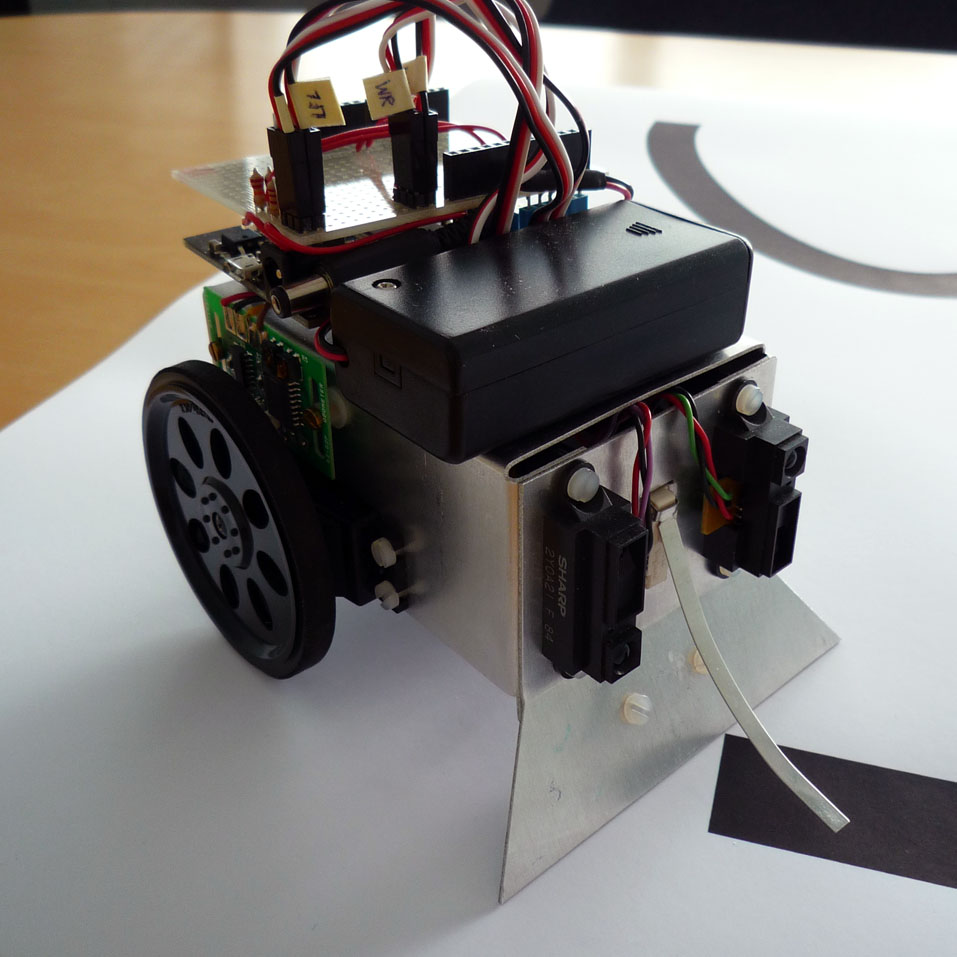
\includegraphics[width=0.3\linewidth]{linefollower/r2g2p_netduino}
      \label{fig:linefollower_sm}
}
\subfigure[A line-follow path]
{
      
\includegraphics[width=0.3\linewidth]{linefollower/map}
      \label{fig:linefollower_3dpath}
}
\subfigure[3D representation of the line-following robot]
{
      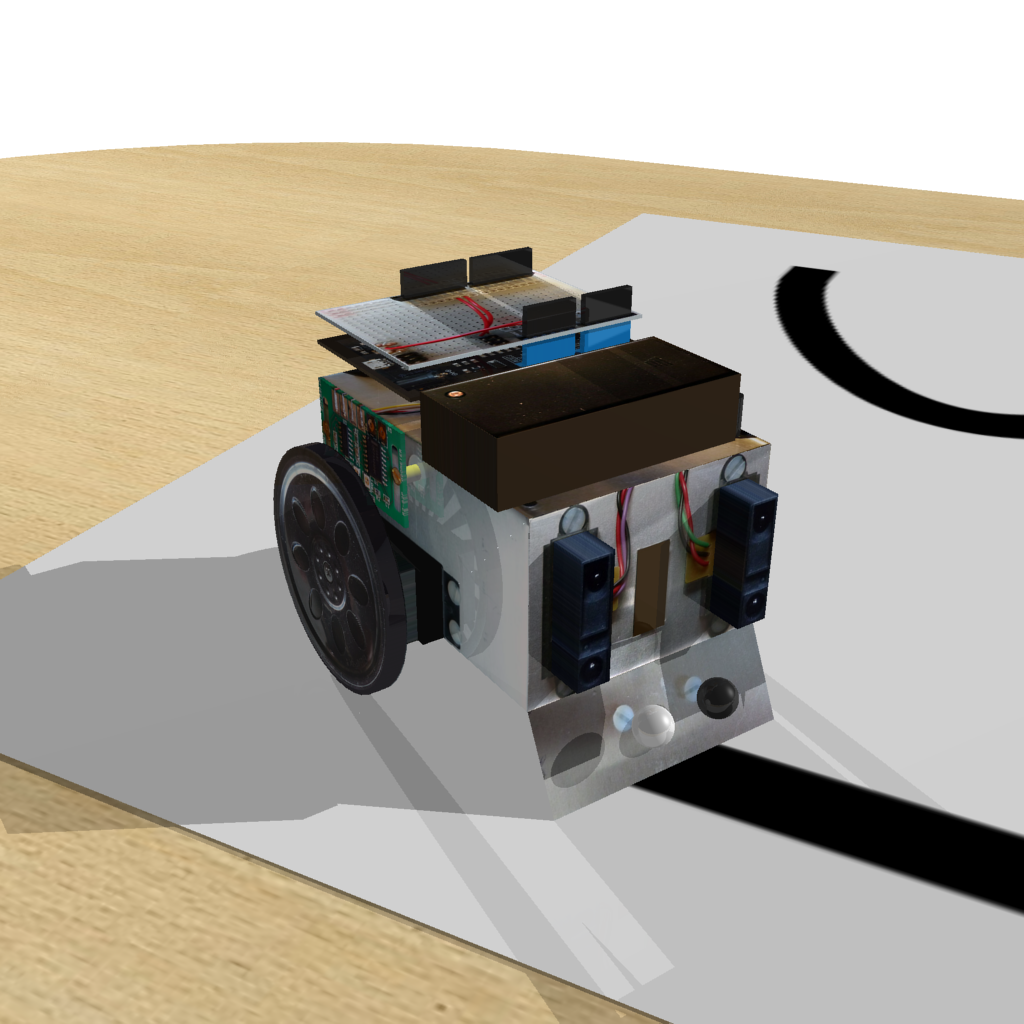
\includegraphics[width=0.3\linewidth]{linefollower/robot_inside}
      \label{fig:linefollower_3d}
}
\caption{The line-following robot}
\label{fig:linefollowoverview}
\end{center}
\end{figure}

\subsection{Usage}
\label{sec:linefollower_usage}

The example is available from the INTO-CPS application menu at \emph{File>Import Example Project} or at  \url{https://github.com/into-cps/case-study\_line\_follower\_robot} in the \emph{master} branch. There are several subfolders for the various elements: DSEs - contains various work in progress DSE scripts to alter CT and DE parameters; \texttt{FMU} -- contains the various FMUs of the study; \texttt{Models} -- contains the constituent models defined using the INTO-CPS simulation technologies; \texttt{Multi-models} -- contains the multi-model definitions and co-simulation configurations -- with 3D and non-3D options, and also with and without the use of replicated FMUs; \texttt{SysML} -- contains the SysML models defined for the study; \texttt{resources} -- various images for the purposes of the readme file; and \texttt{userMetricScripts} -- contains files for DSE analysis. 

The \texttt{case-study\_line\_follower\_robot} folder can be opened in the INTO-CPS application to run the various co-simulations as detailed in this document. To run a simulation, expand one of the multi-models and click `Simulate' for an experiment. 


%\subsection{INTO-CPS Technology}
%
%We demonstrate the use of the INTO-CPS SysML profile in Section~\ref{sec:linefollwerrobot_into_sysml}. Based upon the design architecture defined using the SysML profile, a multi-model is constructed in Section~\ref{sec:linefollwerrobot_into_mm} along with the defined connections.

\subsection{INTO SysML profile}
\label{sec:linefollwerrobot_into_sysml}

\subsubsection*{Non replicated sensors}
The multi-model architecture, defined in the INTO-CPS SysML profile, shows that the \emph{Robot} system is comprised of up to 5 components, as shown in the Architecture Structure Diagram in Figure~\ref{fig:linefollowasd}. This comprises the following components: \emph{Body}, \emph{Sensor1} and \emph{Sensor2} physical components, a \emph{Controller} cyber component and a \emph{3DVisualisation} visualisation component.

\begin{figure}[htb!]
\begin{center}
     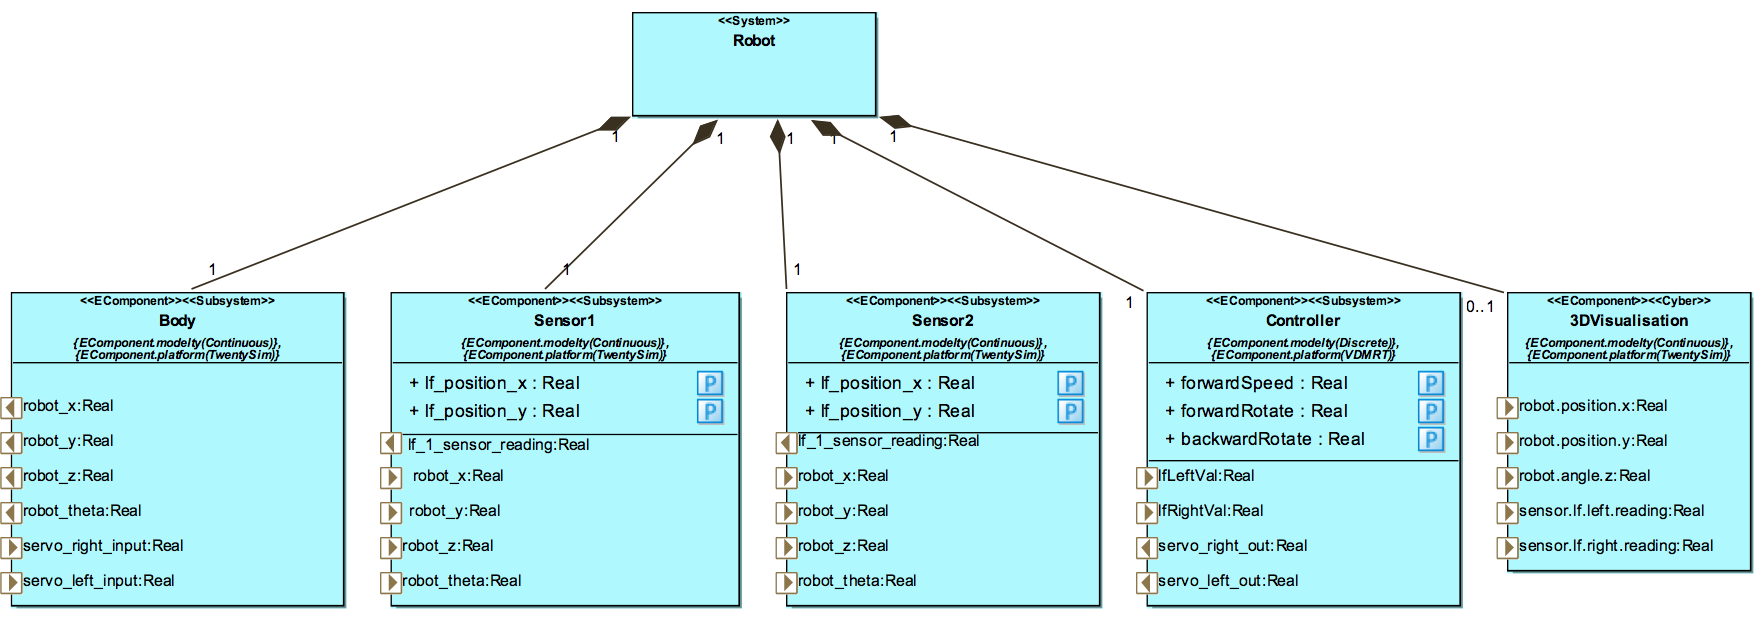
\includegraphics[width=1\linewidth]{linefollower/r2g2p_asd.png} 
\caption{The line-following robot Architecture Structure Diagram}
\label{fig:linefollowasd}
\end{center}
\end{figure}


Two Connection Diagrams are defined. The first, in Figure~\ref{fig:linefollowcd1}, shows connections only between the \emph{Controller}, \emph{Body}, \emph{Sensor1} and \emph{Sensor2} component instances. Broadly speaking: the \emph{Controller} receives sensor readings from both \emph{Sensor1} and \emph{Sensor2} components; the \emph{Controller} in turn sends servo commands to the \emph{Body} component; and finally the \emph{Body} sends the robot position to both sensor components. 

\begin{figure}[htb!]
\begin{center}
     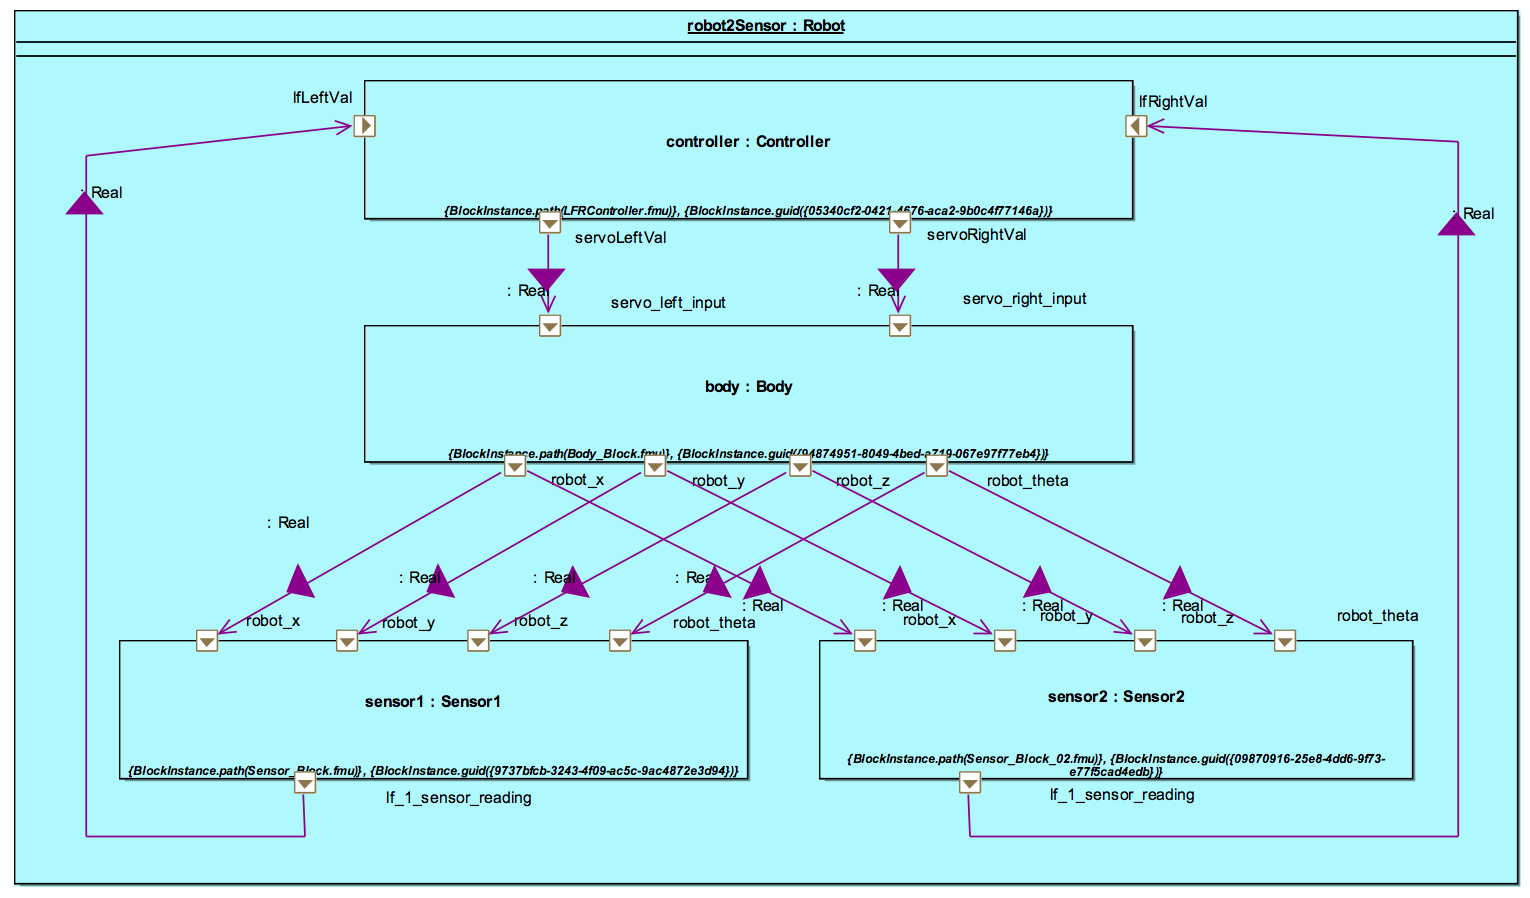
\includegraphics[width=0.9\linewidth]{linefollower/r2g2p_cd_non3d.png} 
\caption{The line-following robot Connections Diagram}
\label{fig:linefollowcd1}
\end{center}
\end{figure}

Figure~\ref{fig:linefollowcd2} shows the alternative CD in which the \emph{3DVisualisation} component is used. In this diagram, the \emph{3DVisualisation} component receives data from the \emph{Body} on the robot position, and the sensor readings from the two sensors. Unlike other examples using the visualisation component type, no additional internal data is required to be exposed by the existing components. 

\begin{figure}[htb!]
\begin{center}
     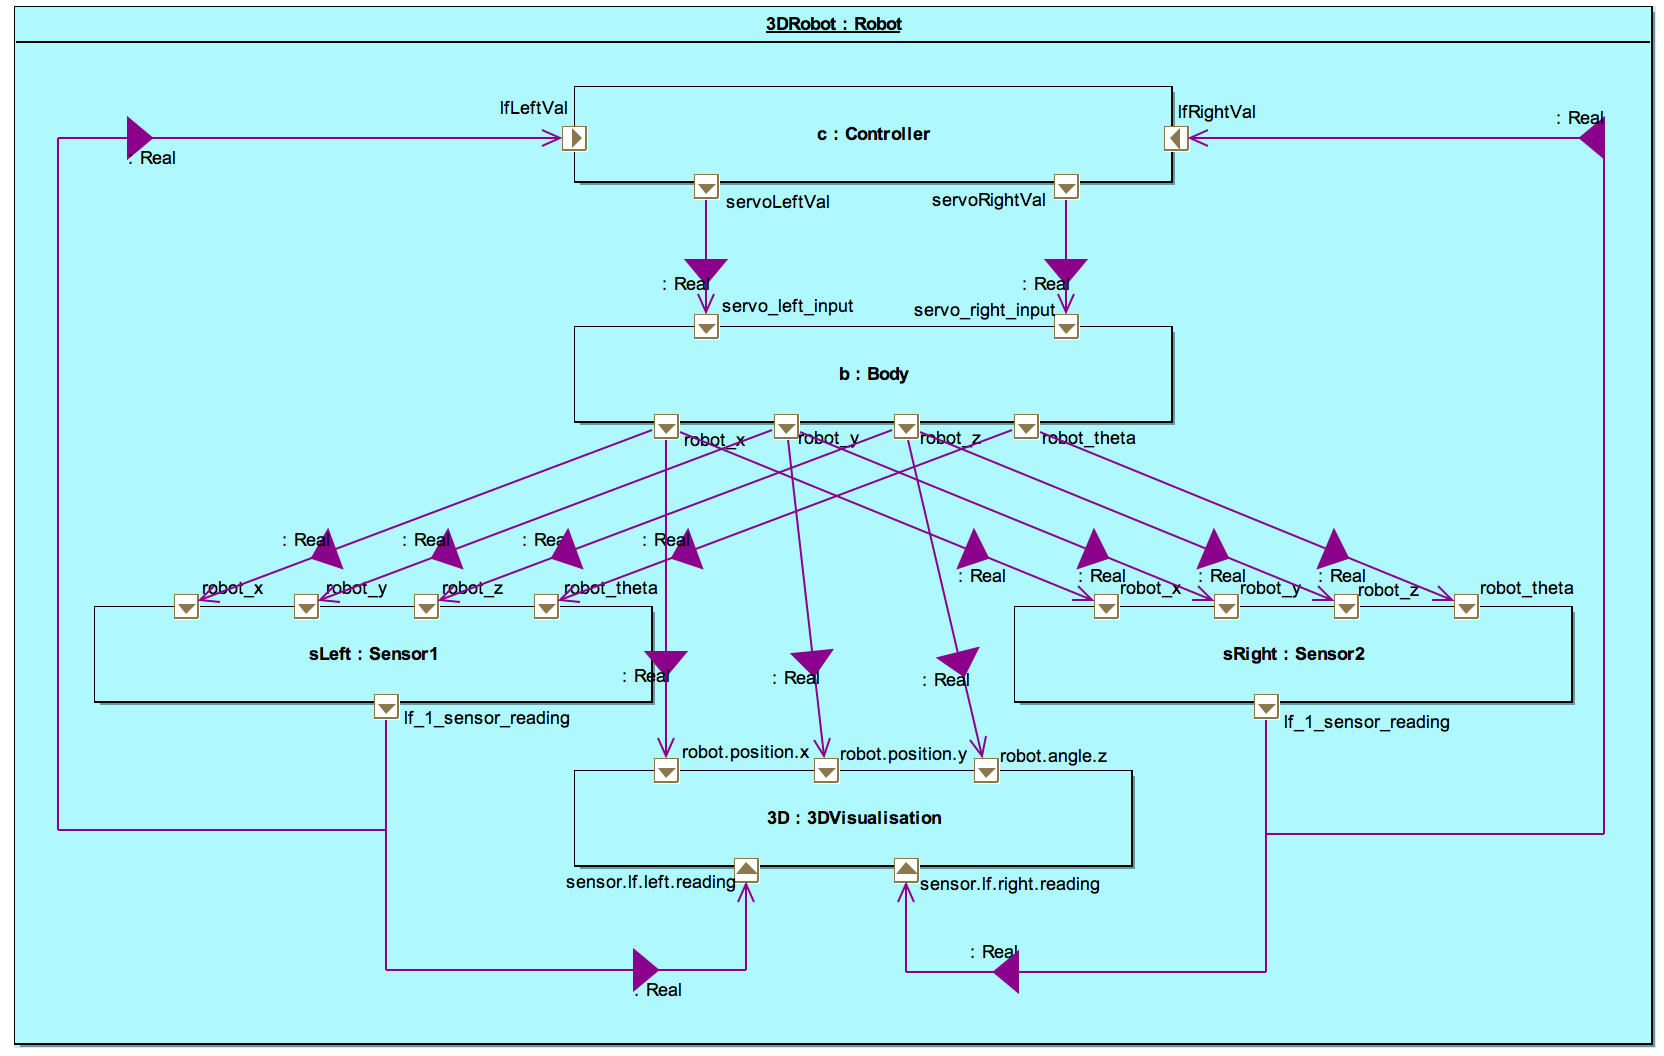
\includegraphics[width=0.9\linewidth]{linefollower/r2g2p_cd_nonrep_3d.png} 
\caption{The line-following robot Connections Diagram}
\label{fig:linefollowcd2}
\end{center}
\end{figure}

\subsubsection*{Replicated sensors}

An alternative architecture has also been defined in which we use replication offered by 20-sim and OpenModelica FMUs. The ASD in Figure~\ref{fig:linefollowasdrep} demonstrates the use of two instances of the same \emph{Sensor} component type.

\begin{figure}[htb!]
\begin{center}
     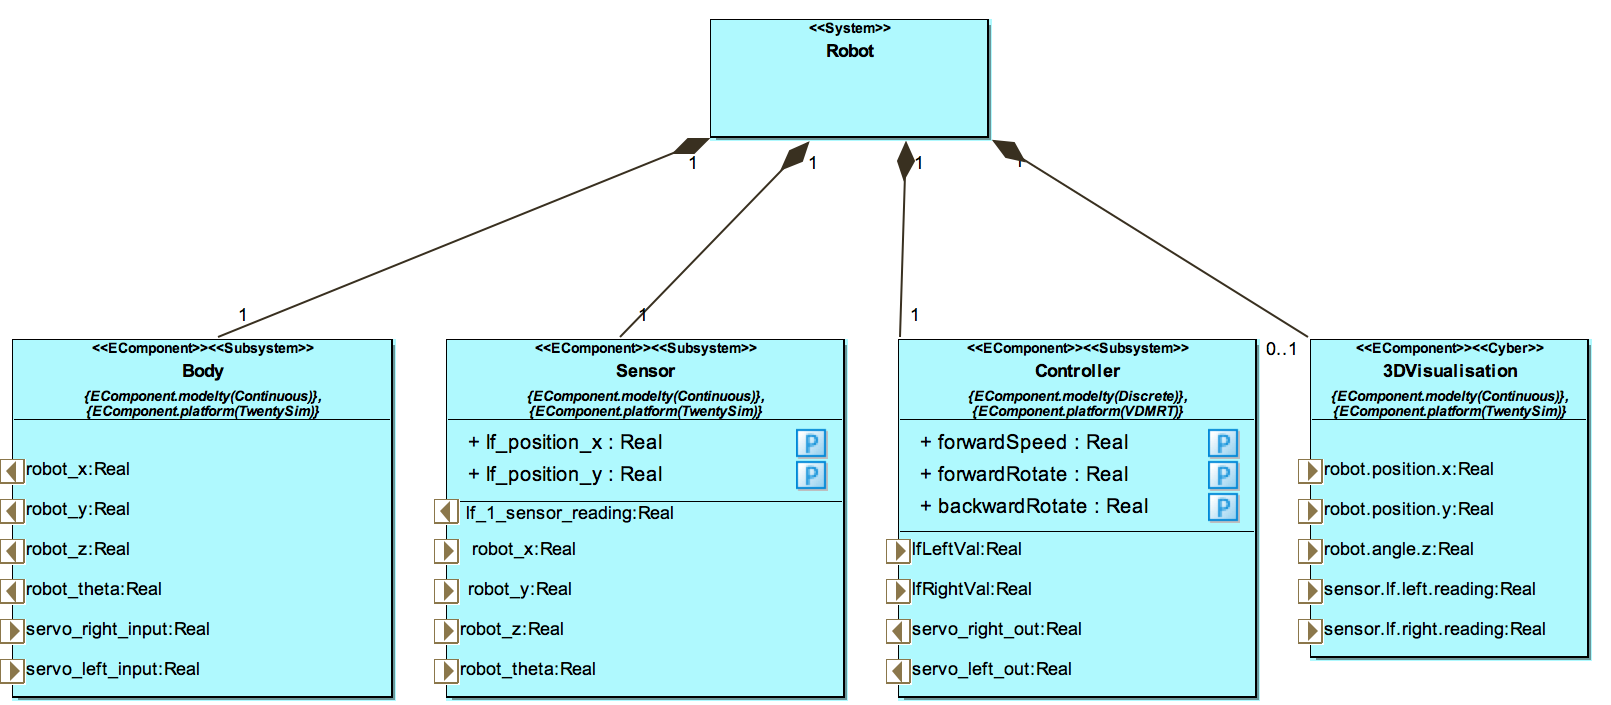
\includegraphics[width=0.8\linewidth]{linefollower/r2g2p_asd_rep.png} 
\caption{The line-following robot Architecture Structure Diagram with replicated sensors}
\label{fig:linefollowasdrep}
\end{center}
\end{figure}

The CDs for this SysML model are similar to the non-replicated sensor model. The only difference is the change of sensor types for the two sensor instances -- this is shown in Figures~\ref{fig:linefollowcdrep1} and~\ref{fig:linefollowcdrep2}.

\begin{figure}[htb!]
\begin{center}
     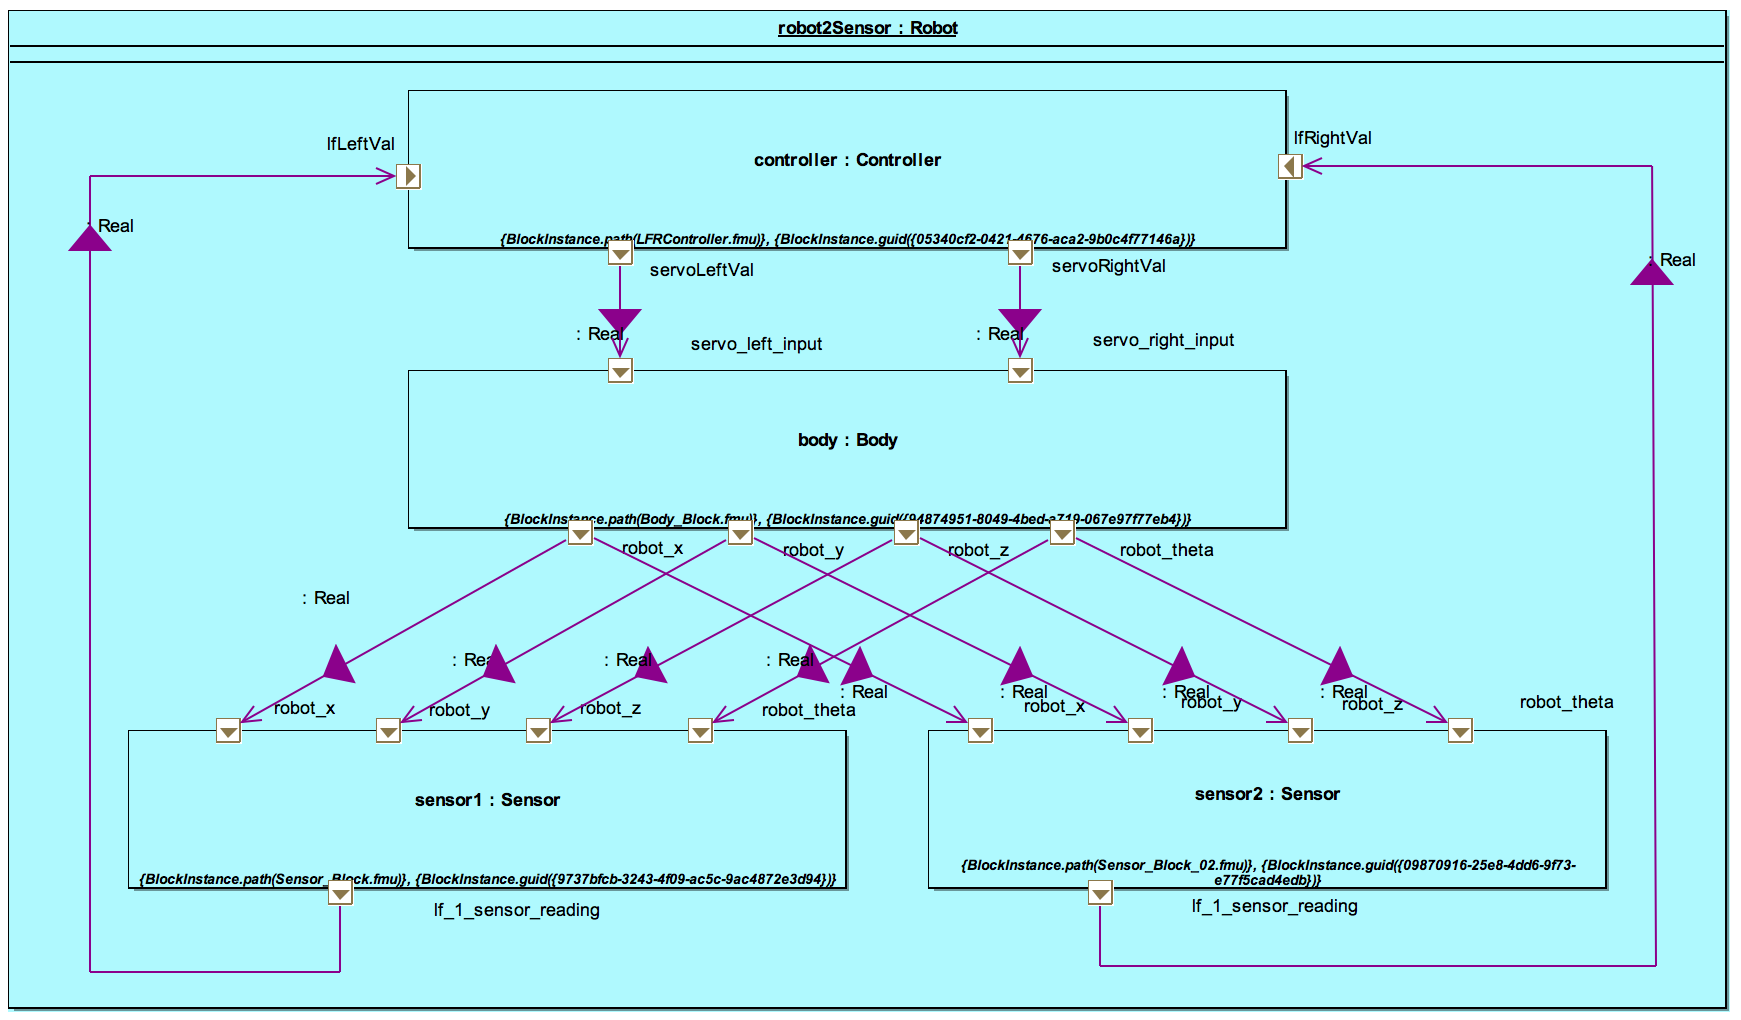
\includegraphics[width=0.9\linewidth]{linefollower/r2g2p_cd} 
\caption{The line-following robot Connections Diagram}
\label{fig:linefollowcdrep1}
\end{center}
\end{figure}

\begin{figure}[htb!]
\begin{center}
     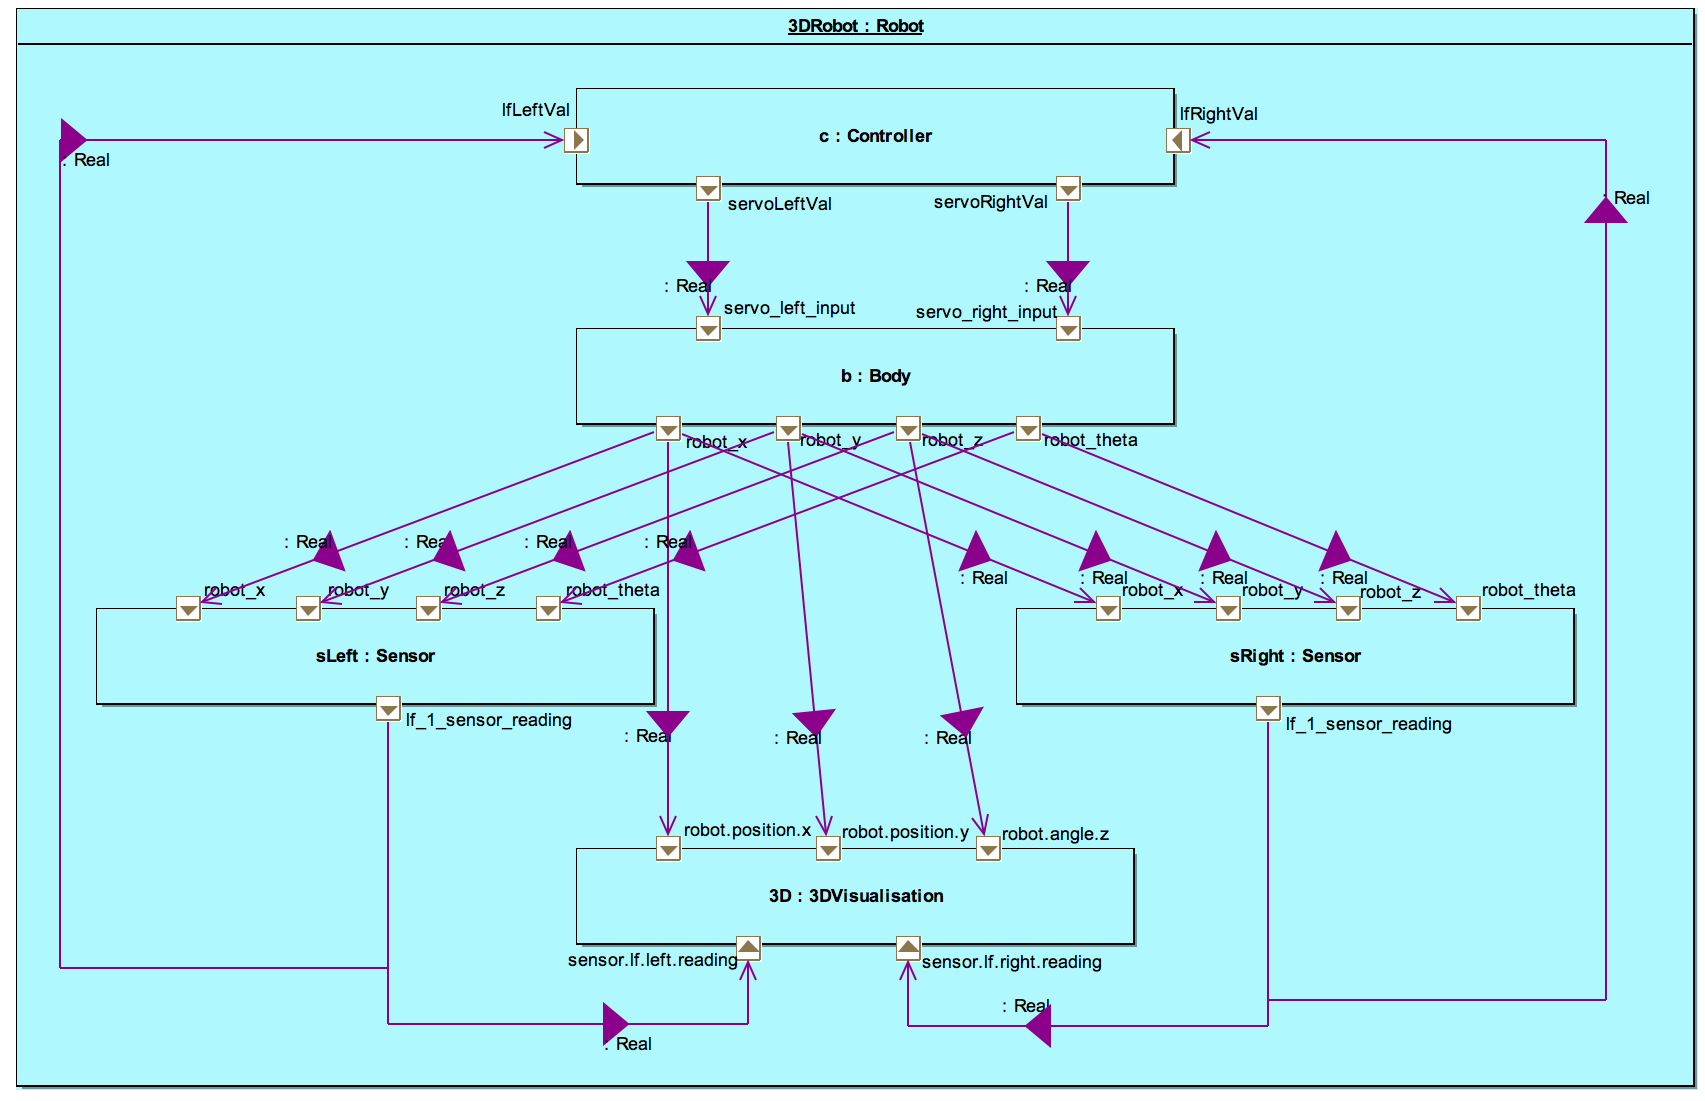
\includegraphics[width=0.9\linewidth]{linefollower/r2g2p_cd_rep_3d} 
\caption{The line-following robot Connections Diagram}
\label{fig:linefollowcdrep2}
\end{center}
\end{figure}


\subsection{Multi-model}
\label{sec:linefollwerrobot_into_mm}

\subsubsection{Models}
%The multi-model produced and analysed using INTO-CPS technology stems from the baseline Crescendo co-model. The multi-model comprises 3 models, splitting the Crescendo model as depicted in Figure~\ref{fig:linefollowsplit}.  This example, therefore is a multi-CT model, with a single DE model. 
%
%\begin{figure}[htb!]
%\begin{center}
%     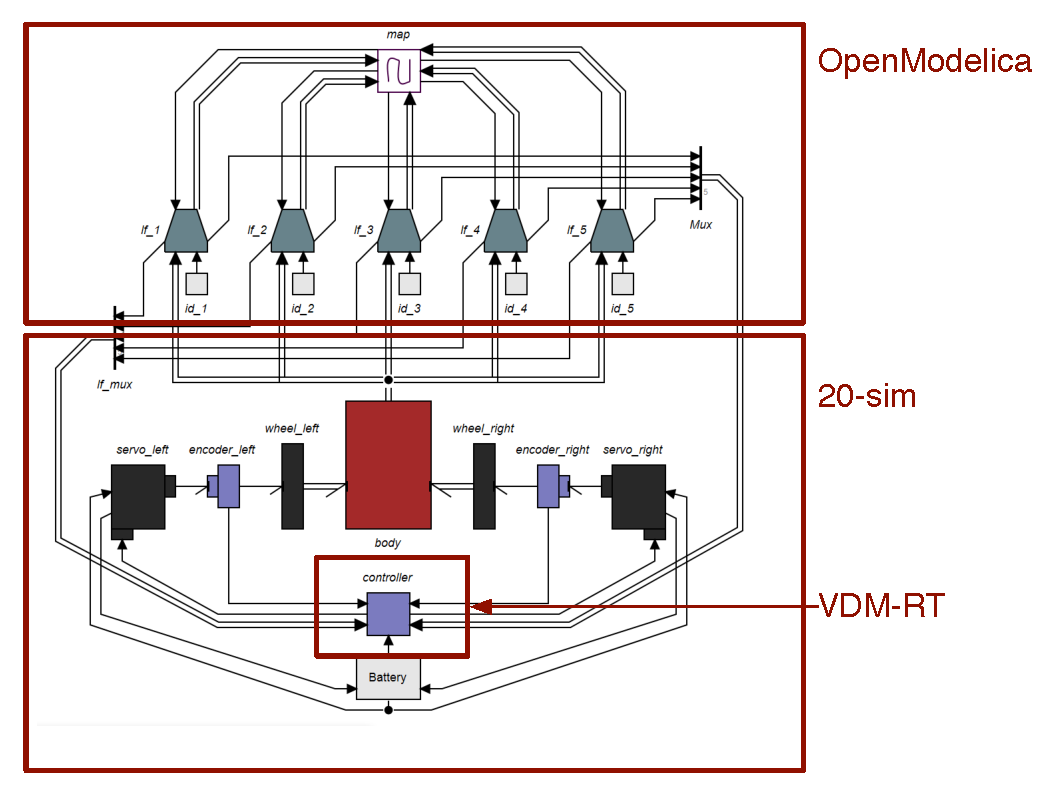
\includegraphics[width=0.65\linewidth]{linefollower/r2g2p_ct_split} 
%\caption{Splitting the line-following robot Crescendo model}
%\label{fig:linefollowsplit}
%\end{center}
%\end{figure}

Based upon the two SysML models, we define four different simulation models: a 20-sim \emph{Body} model; a VDM-RT \emph{Controller} model; a 20-sim \emph{Sensor} models; and one OpenModellica \emph{Sensor} model.  

\begin{description}
\item[Body] To define the 20-sim Body subsystem, Figure~\ref{fig:linefollow20simmod}, we first define a top-level decomposition with a \emph{Body\_Block} and a block to represent the body's \emph{Environment}. 

\begin{figure}[htb!]
\begin{center}
  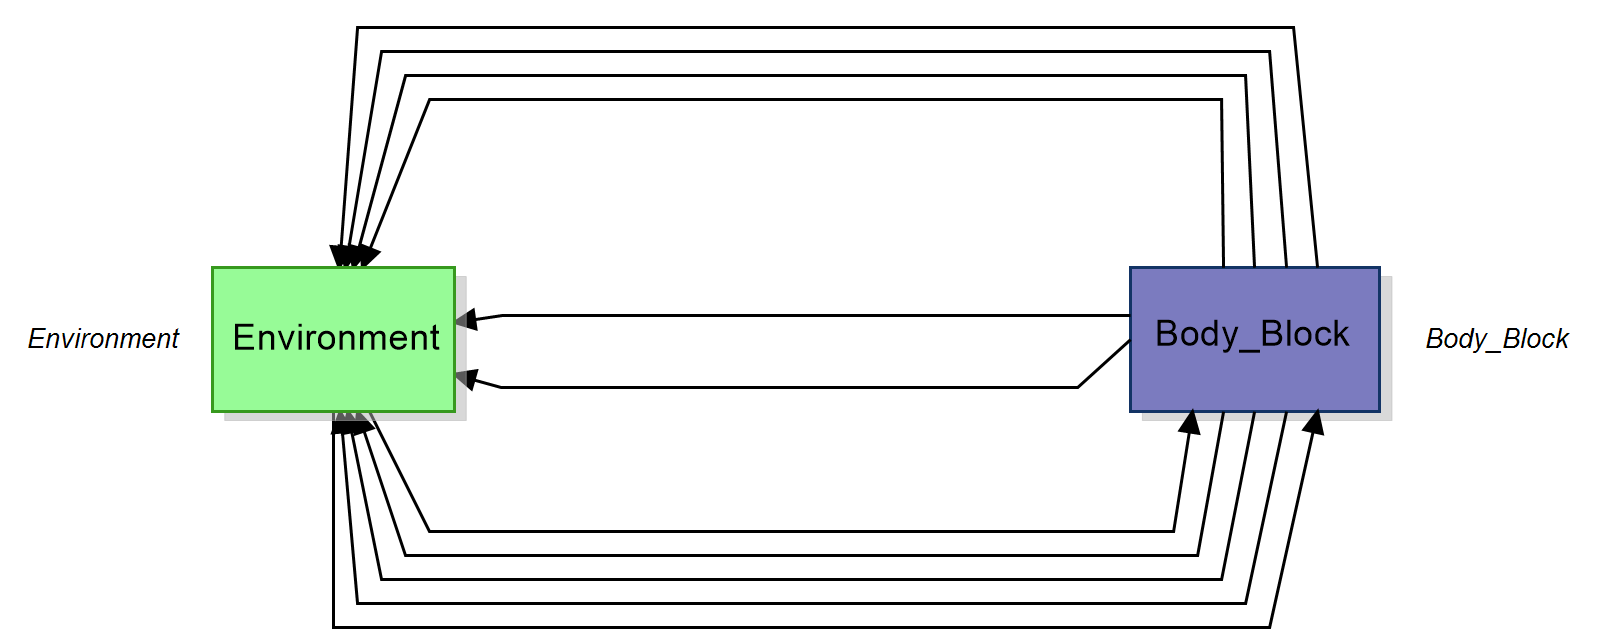
\includegraphics[width=0.65\linewidth]{linefollower/r2g2t_mod2} 
\caption{Top-level 20-sim model of the line-following robot \emph{Body}}
\label{fig:linefollow20simmod}
\end{center}
\end{figure}

Decomposing the \emph{Body\_Block} further, the 20-sim model is defined as in Figure~\ref{fig:linefollowbody20simmm}. Blocks are defined for servos, encoders, wheels, the battery and the body itself. A collection of input and output ports are defined: ports to output the robot position (\emph{robot\_x}, \emph{robot\_y}, \emph{robot\_z} and \emph{robot\_theta}); ports to output wheel rotation values (\emph{wheel\_left\_rotation} and \emph{wheel\_right\_rotation}); a port to output the battery usage (\emph{total\_energy\_used}); and ports for inputting servo power values (\emph{servo\_left\_input} and \emph{servo\_right\_input}).

\begin{figure}[htb!]
\begin{center}
     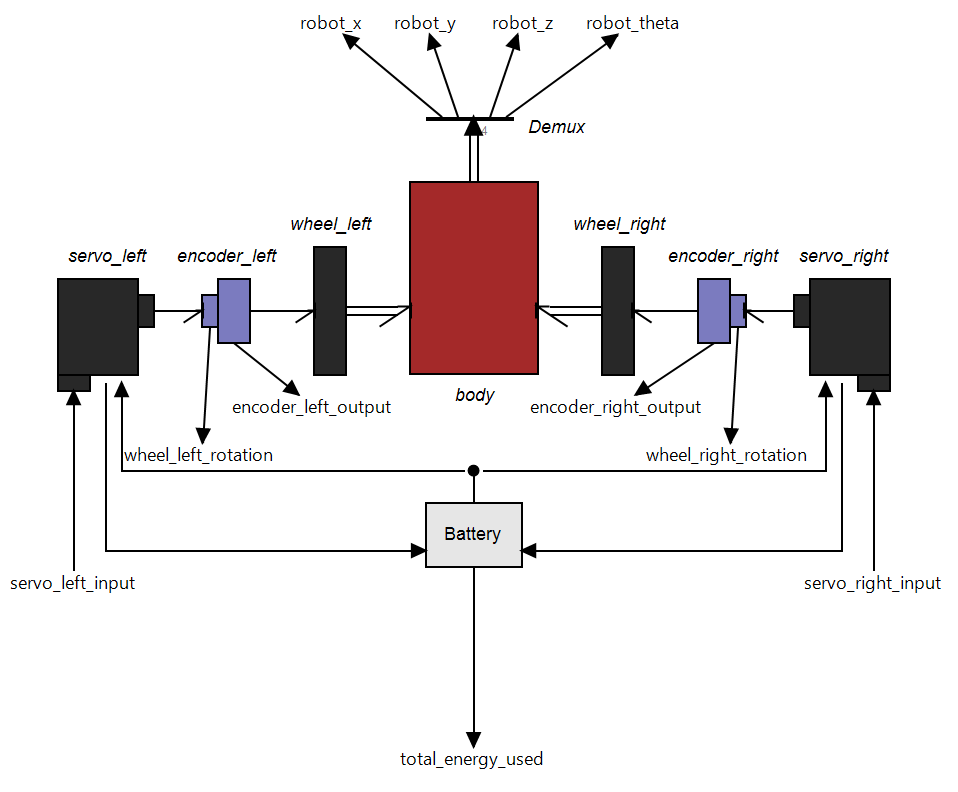
\includegraphics[width=0.7\linewidth]{linefollower/r2g2p_body} 
\caption{20-sim model of the line-following robot \emph{Body}}
\label{fig:linefollowbody20simmm}
\end{center}
\end{figure}



\item[20-sim\_Sensor] The \emph{Sensor\_Block} is shown in Figure~\ref{fig:linefollow20simsensor}.  For the non-replicated version, we change the names of the \emph{Sensor\_Block} to generate different FMUs.

\begin{figure}[htb!]
\begin{center}
 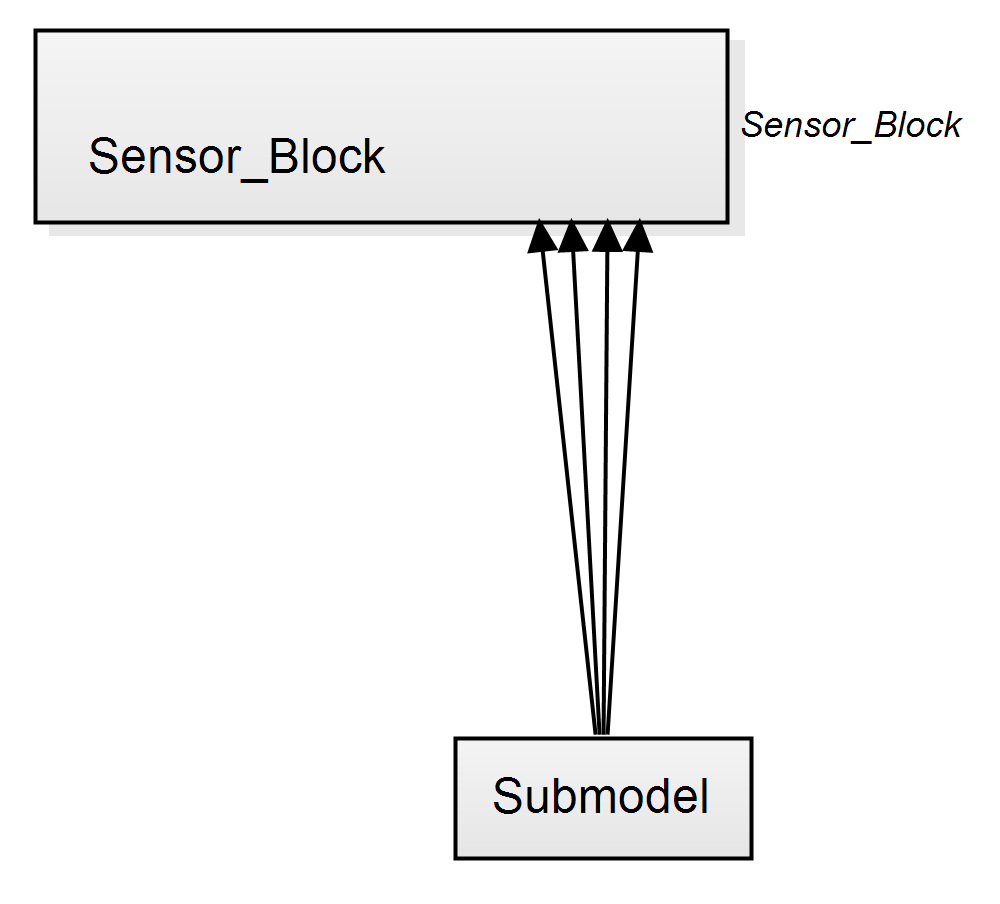
\includegraphics[width=0.45\linewidth]{linefollower/r2g2p_sensor1} 
\caption{Top-level 20-sim model of the line-following robot \emph{Sensor}}
\label{fig:linefollow20simsensor}
\end{center}
\end{figure}

Decomposing the \emph{Sensor\_Block}, we see the internal elements of the sensor -- shown in Figure~\ref{fig:linefollowbody20sensor2}. The sensor receives the robot position from its environment, calculating its position in the world using the \emph{line\_follow\_x} and \emph{line\_follow\_y} design parameters. This position information is passed to the \emph{map} block, which takes a sample of values and passes a raw reading back to the sensors. The sensors then convert this to an 8-bit value, taking into account realistic behaviours: ambient light levels, a delayed response to changes, and A/D conversion noise. The final sensor reading is output on the \emph{lf\_1\_sensor\_reading} port. 

\begin{figure}[htb!]
\begin{center}
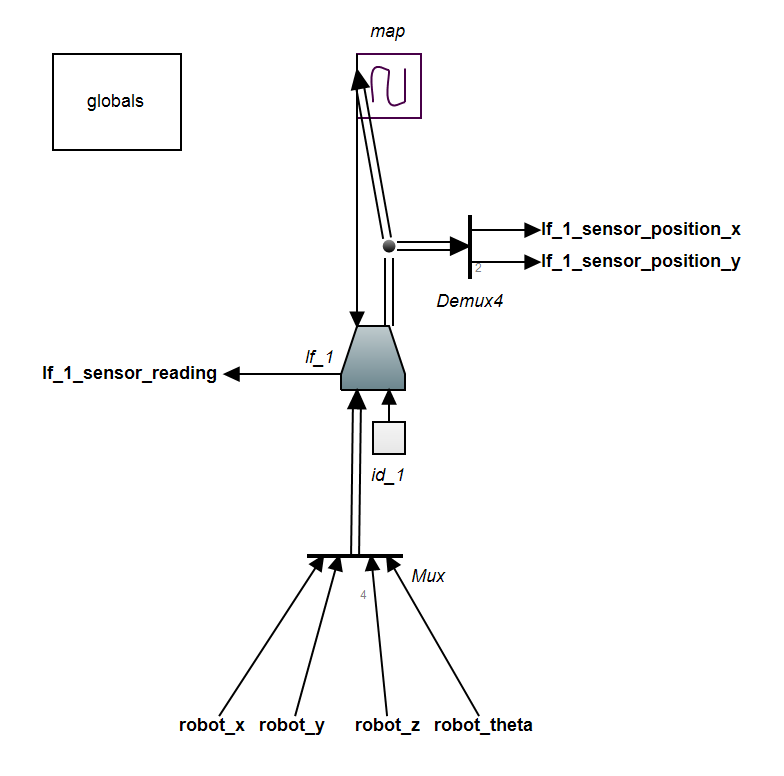
\includegraphics[width=0.5\linewidth]{linefollower/r2g2p_sensor2} 
\caption{20-sim model of the line-following robot \emph{Sensor}}
\label{fig:linefollowbody20sensor2}
\end{center}
\end{figure}

\item[OM\_Sensor] The OpenModelica version of the sensor is provided in the \emph{LineFollower} package. The 
\emph{SensorBlock1.mo} element, shown in Figure~\ref{fig:linefollowbodyOMsensor} corresponds to the 20-sim model shown in Figure~\ref{fig:linefollowbody20sensor2}. The model has the same interface, with internal elements for reflectivity, ambient light, and A/D conversion noise.

\begin{figure}[htb!]
\begin{center}
\subfigure[Top-level view]
{
      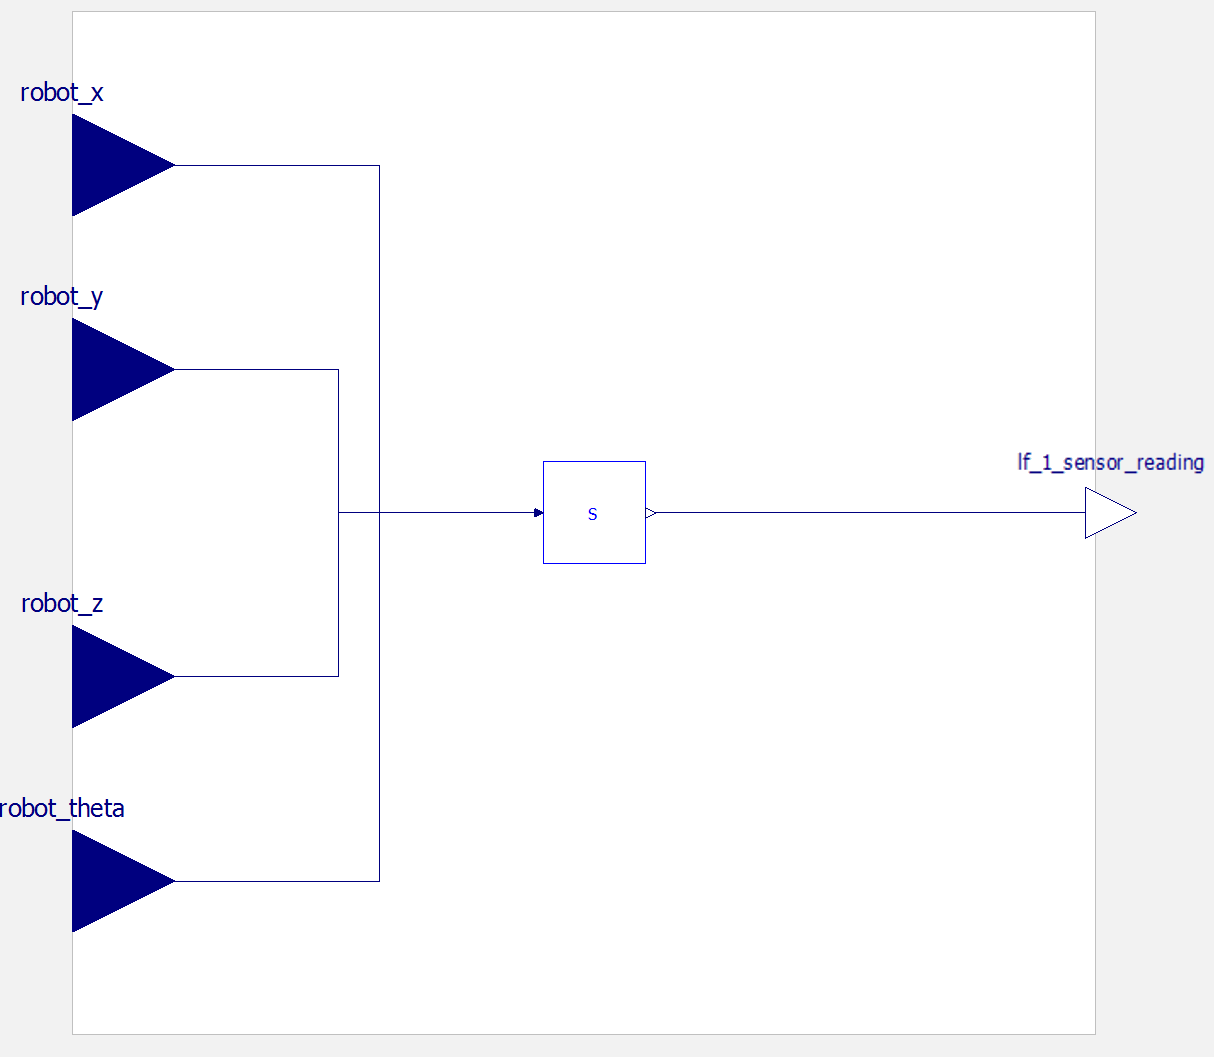
\includegraphics[width=0.45\linewidth]{linefollower/r2g2p_sensor_om_2}
      \label{fig:linefollower_om_s1}
}
\subfigure[Low-level view]
{
      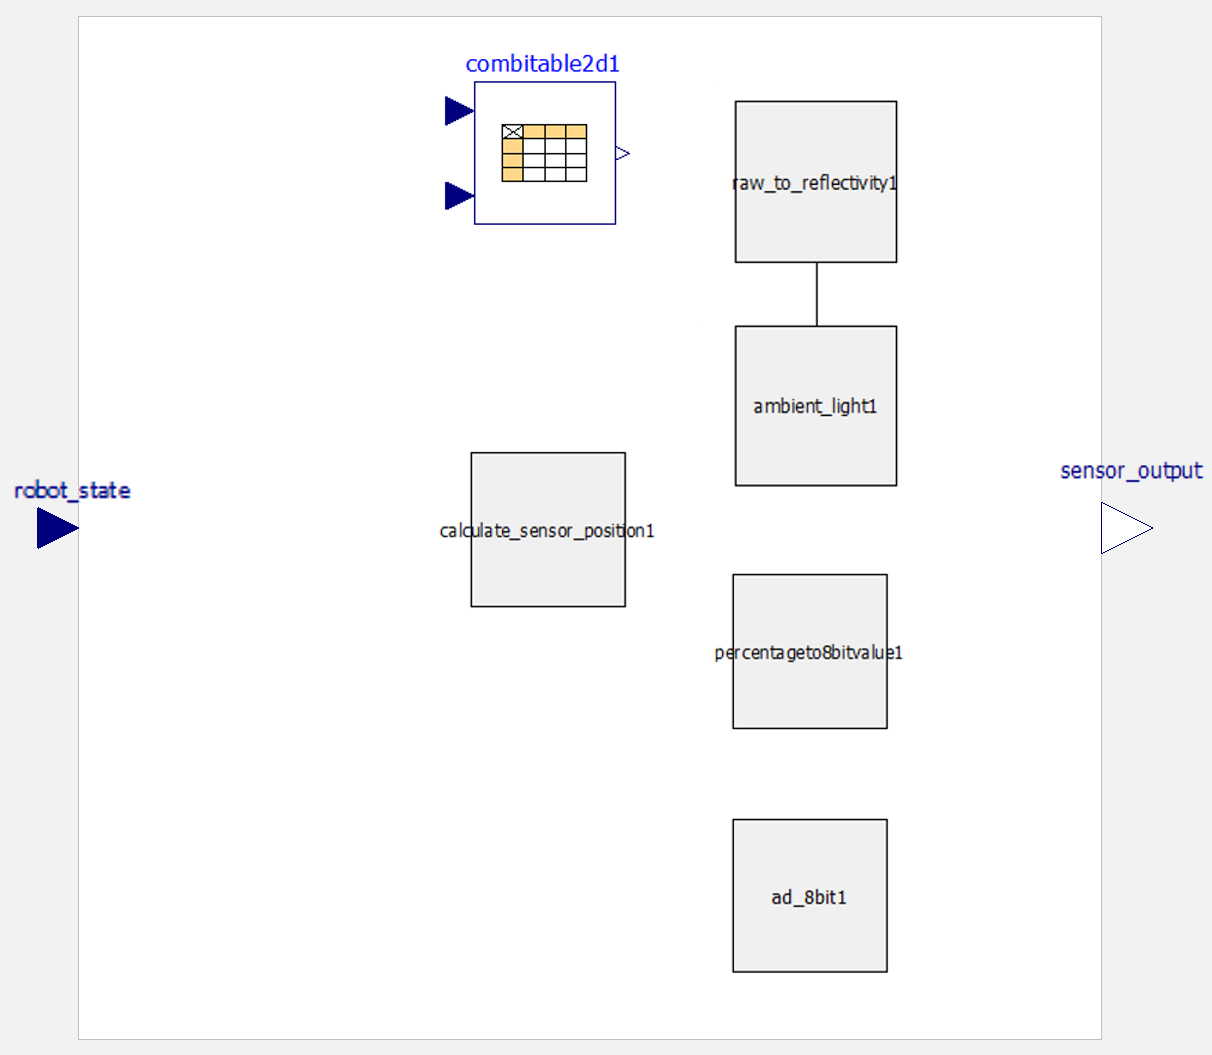
\includegraphics[width=0.45\linewidth]{linefollower/r2g2p_sensor_om}
      \label{fig:linefollower_om_s2}
}
\caption{OpenModelica model of the line-following robot \emph{Sensor}}
\label{fig:linefollowbodyOMsensor}
\end{center}
\end{figure}



\item[Controller] The VDM-RT controller model is conceptually unchanged from the original Crescendo controller. The architecture of this model is in Figure~\ref{fig:linefollowbodyvdm}. The \emph{Controller} model comprises a \emph{System} class which contains a \emph{HardwareInterface} instance which contains references to the inputs, outputs and design parameters. The \emph{System} class also contains a \emph{Controller} class which makes the control decisions. The decisions are based upon sensor readings obtained from two instances of the \emph{RobotSensor} class, and decisions are sent to the two \emph{RobotServo} instances. In this model, a simple algorithm is used: when both sensors see a black line the robot moves forward (both servos are set to the same value), when only the right sensor sees the black line the robot moves left -- and vice-versa.


\begin{figure}[htb!]
\begin{center}
     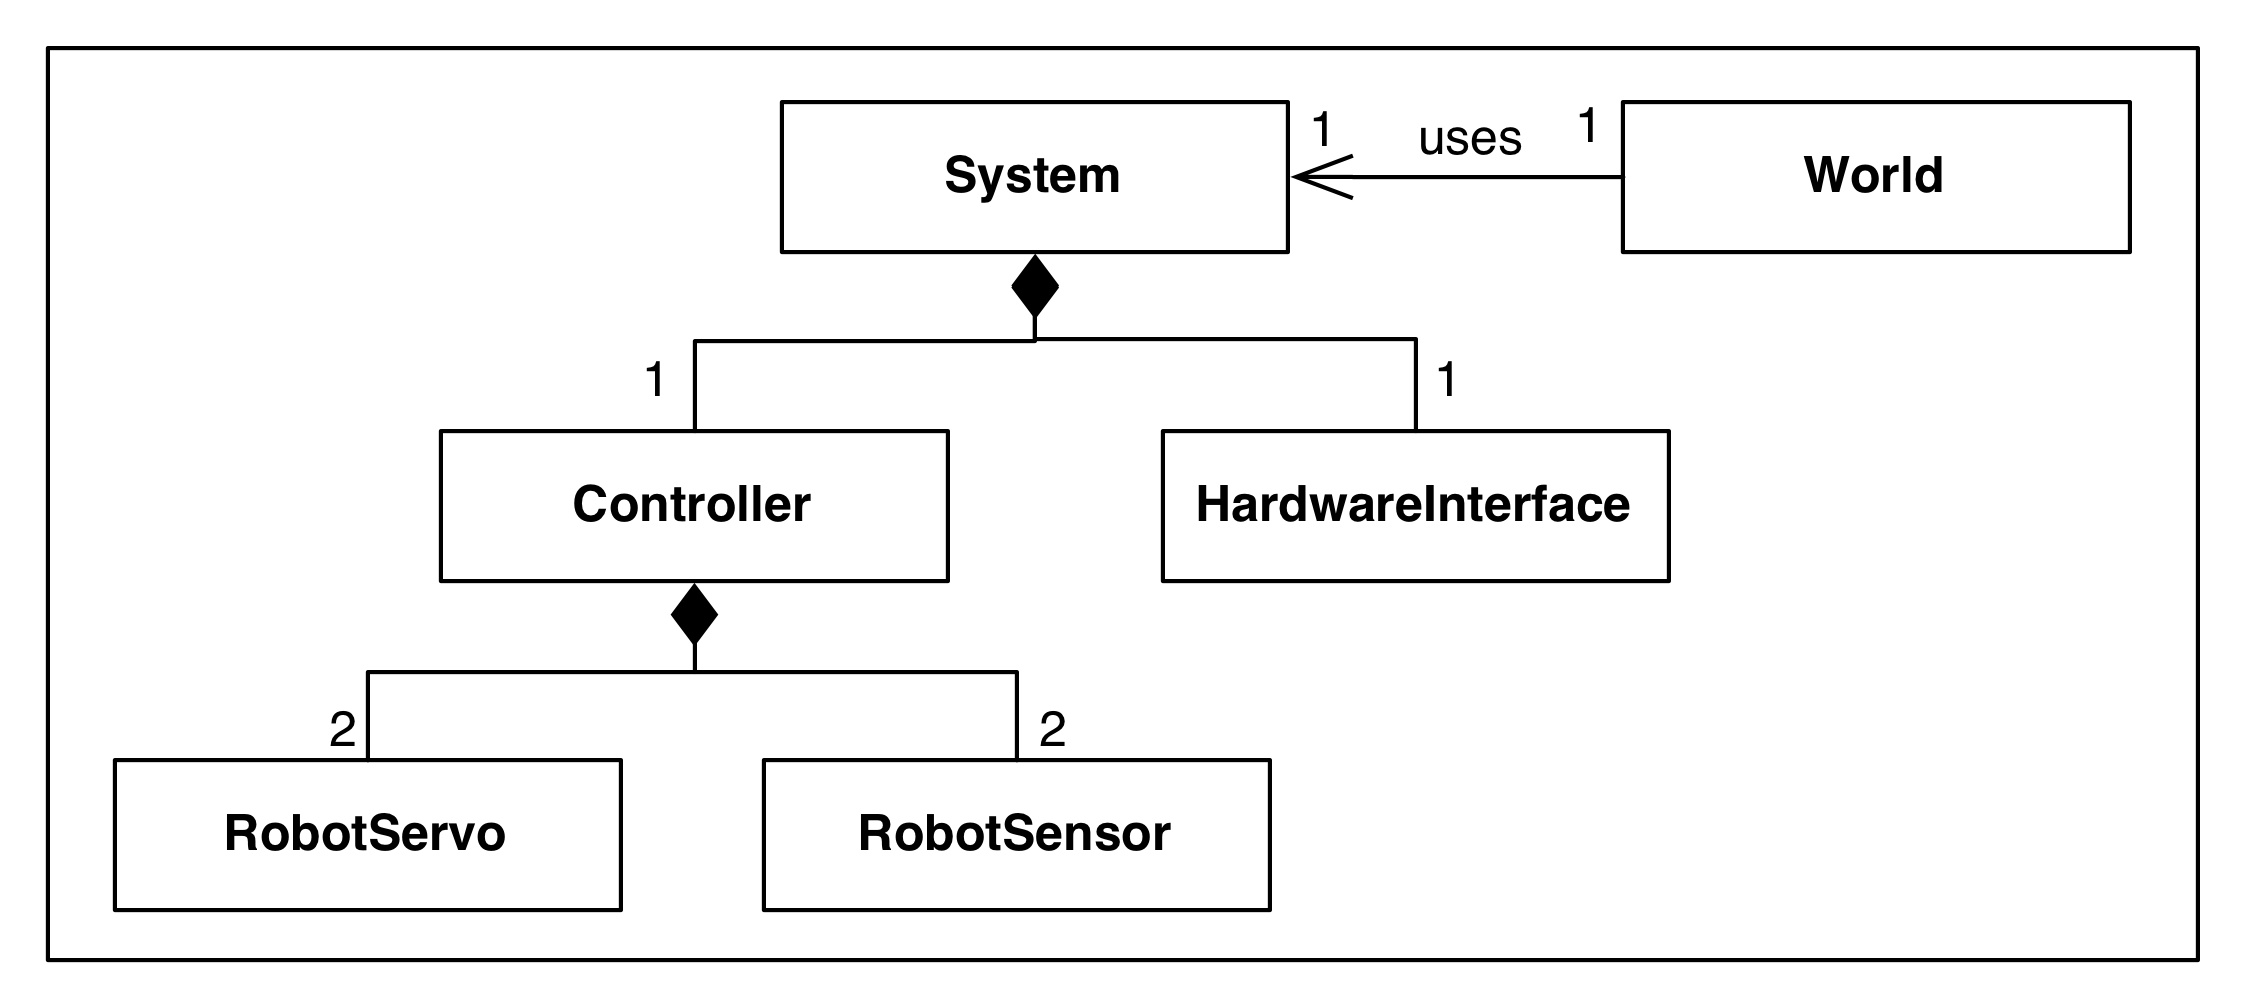
\includegraphics[width=0.8\linewidth]{linefollower/r2g2p_vdm} 
\caption{UML representation of line-following robot \emph{Controller} model}
\label{fig:linefollowbodyvdm}
\end{center}
\end{figure}

\end{description}

\subsubsection{Configuration}

There are several connections between the models in the multi-model.

The first collection of connections is between the Body 20-sim model and the Controller VDM-RT model. In this collection, there are two connections corresponding to signals for the actuators that power the motors for the wheels:
\begin{itemize}
  \item from the \emph{Controller} \texttt{servoLeftVal} variable of type real to the \texttt{servo\_left\_input} port of the \emph{Body}; and
  \item from the \emph{Controller} \texttt{servoRightVal} variable of type real to the \texttt{servo\_right\_input} port of the \emph{Body}. 
\end{itemize} 

The second collection of connections is between the Sensor models and the Controller VDM-RT model. For each sensor there is one connection to the controller to represent inputs from line-following sensors that can detect areas of light and dark on the ground. Therefore for a two-sensor model there are two connections:
 \begin{itemize}
  \item from the \emph{Sensor1}\footnote{Sensor1 is an instance of either the non-replicated \emph{Sensor\_Block1} or the replicated \emph{Sensor\_Block}} \texttt{lf\_1\_sensor\_reading} port to the \emph{Controller} \texttt{lfLeftVal} variable; and 
  \item from the \emph{Sensor2}\footnote{Sensor2 is an instance of either the non-replicated \emph{Sensor\_Block2} or the replicated \emph{Sensor\_Block}} \texttt{lf\_1\_sensor\_reading} port to the \emph{Controller} \texttt{lfRightVal} variable. 
\end{itemize}

  
A third collection of connections exist between the body and the sensors related to the robot position:
 \begin{itemize}
  \item from the \emph{Body} \texttt{robot\_x} port to the \emph{Sensor} \texttt{robot\_x} port; 
  \item from the \emph{Body} \texttt{robot\_y} port to the \emph{Sensor} \texttt{robot\_y} port; 
  \item from the \emph{Body} \texttt{robot\_z} port to the \emph{Sensor} \texttt{robot\_z} port; and 
  \item from the \emph{Body} \texttt{robot\_theta} port to the \emph{Sensor} \texttt{robot\_theta} port. 
\end{itemize}
  
A collection of multi-models   is provided in the study for combinations of 20-sim and OpenModelica models.
  
Several shared design parameters are present also: the separation of the line-following sensors from the centre line, in metres (\emph{line\_follow\_x}); and the distance forward of the line-following sensors from the centre of the robot, in metres (\emph{line\_follow\_y}). In addition, design parameters are set for the controller: the \emph{forwardSpeed} and values for rotation -- \emph{forwardRotate} and \emph{backwardRotate}.
  

\subsection{Co-simulation}
\label{sec:fcu_into_co}

For all these multi-models, co-simulations require approximately 25-30 seconds of simulation to traverse the full map, using a fixed step size of 0.01 seconds. The example has co-simulation set ups for each multi-model and the non-3D models have live stream enabled for the sensed values from sensor1 and sensor2.

\subsection{Analyses and Experiments}
\label{sec:fcu_analyses}

Below we detail some useful experiments to demonstrate features of the INTO-CPS tool chain.

\subsubsection{Change FMUs/parameters}

The case study has several Sensor FMUs. In the multi-model configuration it is possible to swap the FMU allocated to each sensor instance of the multi-model. We can therefore compare the results of co-simulation using a combination of 20-sim sensors (the replicated \emph{Sensor\_Block.fmu}, or \emph{Sensor\_Block1.fmu} and \emph{Sensor\_Block2.fmu}) and OpenModelica sensors (replicated, or some combination of \emph{LineFollower\_Examples\_SensorBlock1.fmu} and \emph{LineFollower\_Examples\_SensorBlock2.fmu}). 

In addition, there are parameters defined for the two sensors (an x and y position \texttt{lf\_position\_x} and \texttt{lf\_position\_y}), and of the controller (forward and rotational speeds \emph{forwardSpeed}, \emph{forwardRotate} and \emph{backwardRotate}). Experiments may be carried out by defining different values for these to model different placement of the sensors on the robot and altering the robot speeds,. 

\subsubsection{Simulations due to previous results}

Simulations can be replayed using different design parameter values to change the position of the robot sensors. Changing these parameters amounts to changing the design of the robot - some value pairs will produce robots which perform in some way better (e.g. have a faster lap time) and others will result in robots which cannot follow the line.

\subsubsection{Design Space Exploration}

Several Design Space Exploration experiments have been included in this pilot. They are described in more detail in Deliverable D5.3e~\cite{INTOCPSD5.3e}, and we give an overview of the different experiments here. 

\begin{description}
   \item[lfr-2sensorPositions:] This experiment uses four design parameters, but only varies one. The \texttt{lf\_position\_y} of \emph{sensor1} may be either $0.07$ or $0.13$. Four objective scripts are used: \emph{meanSpeed}, \emph{lapTime}, \emph{maxCrossTrackError} and \emph{meanCrossTrackError}. The Pareto ranking only uses the \emph{lapTime} and \emph{meanCrossTrackError} objectives; these determine the time taken for the robot to perform one lap of the map, and also the mean error the robot makes when following the line. 
   
   \item[lfr-8controllerValues:] This experiment uses and varies three parameters. These parameters are all on the cyber-side of the multi-model -- effecting the robot speeds set by the controller. For each (\texttt{forwardSpeed}, \texttt{forwardRotate} and \texttt{backwardRotate}), two possible values are defined - giving a design space of 8 designs. The same four objective scripts are used as above with the same Pareto ranking.
   
   \item[lfr-16sensorPositionsConstrained:] This experiment is a more complex version of the \textbf{lfr-2sensorPositions} experiment in that it varies all four design parameters -- the \texttt{lf\_position\_x} and \texttt{lf\_position\_y} coordinates of both \emph{sensor1} and \emph{sensor2}. Two possible values are defined for each parameter -- giving a 16-design space. A constraint is defined for the parameters, which limits this design space to include only those designs which have the same y coordinate and the same absolute x coordinate. The same four objective scripts are used as above with the same Pareto ranking.
   
   \item[lfr-216controllerValues:] This expands the \textbf{lfr-8controllerValues} experiment, providing 6 speed values for the Controller parameters (\texttt{forwardSpeed}, \texttt{forwardRotate} and \texttt{backwardRotate}), producing a design space of 216 designs. The same four objective scripts are used as above with the same Pareto ranking.
   
   \item[lfr-2187ControllerAndSensors:] The final experiment combines DSE on both DE and CT models. Providing an insight into the possibility to trade-off between development effort on the cyber or physical side. In this experiment there are 3 possible positions for each of the the \texttt{lf\_position\_x} and \texttt{lf\_position\_y} coordinates of both \emph{sensor1} and \emph{sensor2}, and also 3 values for the  Controller parameters (\texttt{forwardSpeed}, \texttt{forwardRotate} and \texttt{backwardRotate}). This produces a design space of 2187 designs. The same four objective scripts are used as above with the same Pareto ranking.
   
\end{description}

\subsubsection{Test Automation and Model Checking}
\label{sec:lfr_ta}
\graphicspath{ {linefollower/TA/} }

In this pilot study, we apply test automation only to the controller, instead of the system in the FCU study. The continuous body and sensors are rather complex in order to be modelled in a test model in SysML in Modelio by state machine diagrams. Therefore, only the discrete part \emph{Controller} will be tested. In addition, the \emph{Controller} is a simplified version which is similar to the VDM model in \emph{LFRController.fmu}. In this model, the parameters $forwardSpeed$, $forwardRotate$ and $backwardRotate$ are fixed to 4.0, 5.0 and 1.0 respectively. We implement a SUT manually in C. Then model checking is applied to check a couple of properties of the test model, and finally test automation to test whether the SUT is a correct implementation of the test model.

\paragraph{Test Model}
The overall architecture and connection diagrams of this test model are omitted for brevity. The \emph{SystemUnderTest} includes only one block \emph{LFR\_CTRL}. 
\subparagraph{Inputs and Outputs}
The \emph{SystemUnderTest} receives the following inputs (stimuli) from the \emph{TestEnvironment}:
\begin{itemize}
    \item $sensorLeftVal$ %: the reading of the left sensor; 
    \item $sensorRightVal$ %: the reading of the right sensor.
\end{itemize}

The \emph{SystemUnderTest} provides the following observable outputs to the \emph{TestEnvironment}:
\begin{itemize}
    \item $servoLeft$ %: the signal to the left actuator (to drive the left wheel);
    \item $servoRight$ %: the signal to the right actuator (to drive the right wheel).
\end{itemize}

\subparagraph{Constant Variables and Local Variables}
Preliminarily, we intend to define three constant variables $forwardSpeed$, $forwardRotate$ and $backwardRotate$ of which the access model property is set as \T{Read}. Then in the state machine diagram of \emph{LFR\_CTRL}, we use these variables to refer to constants. However, these constant variables are not supported in RT-Tester. Their initial values are all set to 0 when parsing the test model. Alternatively, we can initialise them to constants in the first state just after the \T{Init} state, or just use hard-coded constants in the test model (the way used in this study).

Another two local variables $preServoLeft$ and $preServoRight$ are declared to store previously output values of $servoLeft$ and $servoRight$ separately. And their access model property is set to \T{Read/Write}.

\subparagraph{State Machine Diagram}
The state machine diagram of \emph{FCU\_CTRL} is given in Figure~\ref{fig:lfr-sm-diagram}. It is worth noting that
\begin{itemize}
    \item This model is based on a very basic variation of the controller and it only provides four possible outputs.
    \item The texts in blue actually are not a part of the model and they are annotations only to illustrate associated expression for each guarded transition (because the expressions cannot be seen from the diagram directly).
    \item When both $sensorLeftVal$ and $sensorRightVal$ are larger than or equal to $150$, our model outputs the previously stored $preServoLeft$ and $preServoRight$. It means the outputs have not changed. 
\end{itemize}
\begin{figure}[htb!]
    \centering
  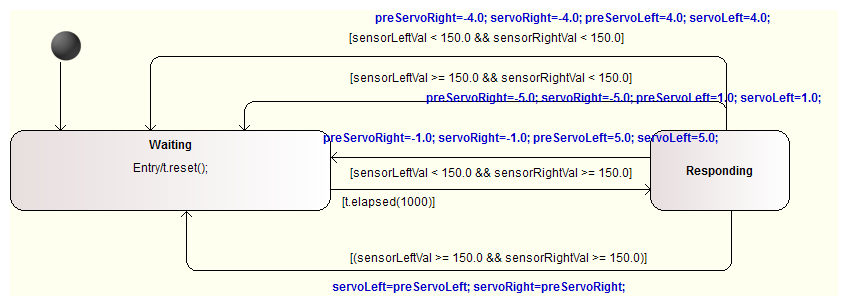
\includegraphics[width=1.0\textwidth]{lfr_sut_sm}
    \caption{State Machine Diagram of LFR Controller}
    \label{fig:lfr-sm-diagram}
\end{figure}


\paragraph{A Manual Implementation of SUT in C}

The source code is listed as follows.
\lstset{language=C,
    basicstyle=\footnotesize\ttfamily,
    keywordstyle=\color{blue}\ttfamily,
    stringstyle=\color{red}\ttfamily,
    commentstyle=\color{green}\ttfamily,
    morecomment=[l][\color{magenta}]{\#},
    tabsize=2
}

\begin{lstlisting}
#include <stdio.h>
#include <sys/time.h>
#include <sys/types.h>
#include "lfr_ctrl.h"

#define FORWARDSPEED    4.0f
#define FORWARDROTATE   5.0f
#define BACKWARDROTATE  1.0f

#define SENSORVAL       150.0f

#define _ms( t ) ( (t) * 1000 )
float preServoRight = 0;
float preServoLeft = 0;

VSTimer_t t;

void reset( VSTimer_t* timer)
{
  struct timeval now;
  ti_gettimeofday( &now, NULL );
  *timer = now.tv_sec * 1000000 + now.tv_usec;
}

BOOLEAN elapsed( VSTimer_t* timer, long usec )
{
  struct timeval now;
  long long usec_now;

  ti_gettimeofday( &now, NULL );
  usec_now = now.tv_sec * 1000000 + now.tv_usec;
  return ( ( usec_now - (*timer) ) >= usec );
}

int firstCall = 1;

/** Initialize SUT */
void sut_init()
{
    preServoLeft    = 0;
    preServoRight   = 0;
    reset(&t);
}

/** Run SUT (one step) */
void sut_run(float sensorLeftVal, float sensorRightVal, 
    float* servoLeft, float* servoRight)
{
    if(firstCall) 
    {
        if(!elapsed(&t, _ms(1002))) 
        {
            *servoRight = preServoRight;
            *servoLeft = preServoLeft;
            return;
        }
    }
    else 
    {
        if(!elapsed(&t, _ms(1000))) 
        {
            *servoRight = preServoRight;
            *servoLeft = preServoLeft;
            return;
        }
    }

    firstCall = 0;
    reset(&t);

    if(sensorLeftVal < SENSORVAL) 
    {
        if(sensorRightVal < SENSORVAL) 
        {
            preServoRight = *servoRight = -FORWARDSPEED;
            preServoLeft = *servoLeft = FORWARDSPEED;
        }
        else //if(sensorRightVal >= SENSORVAL)
        {
            preServoRight = *servoRight = -BACKWARDROTATE;
            preServoLeft = *servoLeft = FORWARDROTATE;
        }
    }
    else // if(sensorLeftVal >= SENSORVAL)
    {
        if(sensorRightVal < SENSORVAL) 
        {
            preServoRight = *servoRight = -FORWARDROTATE;
            preServoLeft = *servoLeft = BACKWARDROTATE;
        }
        else // if(sensorRightVal >= SENSORVAL)
        {
            *servoRight = preServoRight;
            *servoLeft = preServoLeft;
        }
    }

    return;
}
\end{lstlisting}
We define the $reset$ and $elapsed$ functions to reset the time variable $t$ and check where the specified time has elapsed or not. The controller is mainly idle (it could not process inputs but just return previously stored outputs). But every one second, it starts to process inputs and return corresponding outputs. It is worth noting that in the first call of the \emph{sut\_run}, we have additional two ms delay. The reason is given later.

\paragraph{Model Checking}
Model checking can be applied to the test model to check if it satisfies the properties. In order to use bounded model checking in the INTO-CPS app, we set the bounded steps ``BMC steps'' to 50. The properties below are checked to hold in 50 steps.

\begin{description}
    \item[P0] Livelock property by the \B{Check Mode} function on RT-Tester.
\begin{verbatim}
Check static model semantics ...done.
- IMR.SystemUnderTest.lfrCTRL...  [PASS]
- IMR.TestEnvironment... [PASS]

=================================================================
|              Livelock report                                  |
=================================================================
IMR.SystemUnderTest.lfrCTRL.................................[PASS]
IMR.TestEnvironment.........................................[PASS]
\end{verbatim}

    \item[P1] Check all outputs are always within their valid range.
\begin{align*}
    & Globally \left(\left[
        \begin{array}[]{l}
        -5 \leq IMR.servoLeft \land IMR.servoLeft \leq 5 \land \\
        -5 \leq IMR.servoRight \land IMR.servoRight \leq 5
        \end{array}
        \right]\right) &
\end{align*}
    \item[P2] The value of $servoLeft$ is always larger than or equal to 0 but that of $servoRight$ is always less than or equal to 0. 
\begin{align*}
    & Globally \left(
        \begin{array}[]{l}
            \left[\_timeTick == 0\right] \lor \\
            \left[\_timeTick > 0 \land IMR.servoLeft \geq 0 \land IMR.servoRight \leq 0 \right]
        \end{array}
    \right) &
\end{align*}
    \item[P3] If we use constant variables rather than hard-coded constants, we can check they will never be changed. 
\begin{align*}
    & Globally \left(
        \begin{array}[]{l}
            \left[\_timeTick == 0\right] \lor \\
            \left[\_timeTick > 0 \land forwardSpeed == 4.0\right]
        \end{array}
    \right) &
\end{align*}
\end{description}

\paragraph{Test Results}
\subparagraph{User Defined Test Cases}

We use user defined test cases by LTL formulas in RT-Tester to define a test goal that all combinations of inputs shall be covered. This goal is illustrated in Figure~\ref{fig:lfr_mbtconf}. Then the solver will generate a test data generation report that includes test goals, explicitly and implicitly covered test coverage cases, signal configurations, and test stimulations and expected behaviour. This test covers all basic control state coverage test cases (3), all transition coverage test cases (5), and 4 MCDC coverage test cases in 12. The generated test input sequence is shown in Figure~\ref{fig:lfr_test_seq}.
\begin{figure}[htb!]
    \centering
	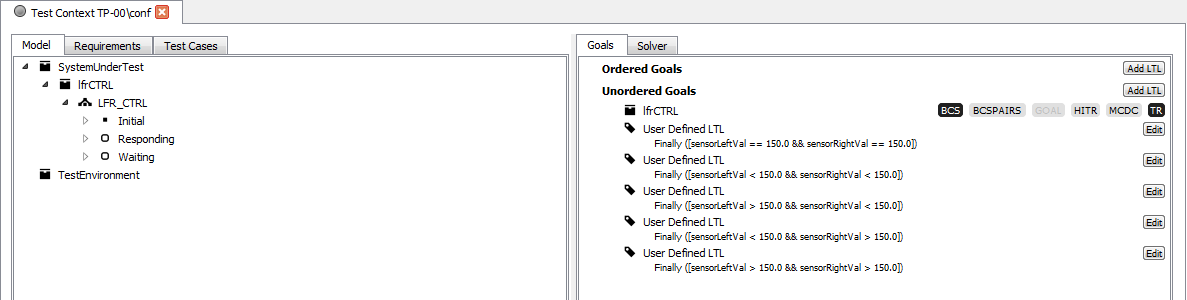
\includegraphics[width=1.0\textwidth]{lfr_mbtconf}
    \caption{Test Goal Configuration of LFR}
    \label{fig:lfr_mbtconf}
\end{figure}

\begin{figure}[htb!]
    \centering
	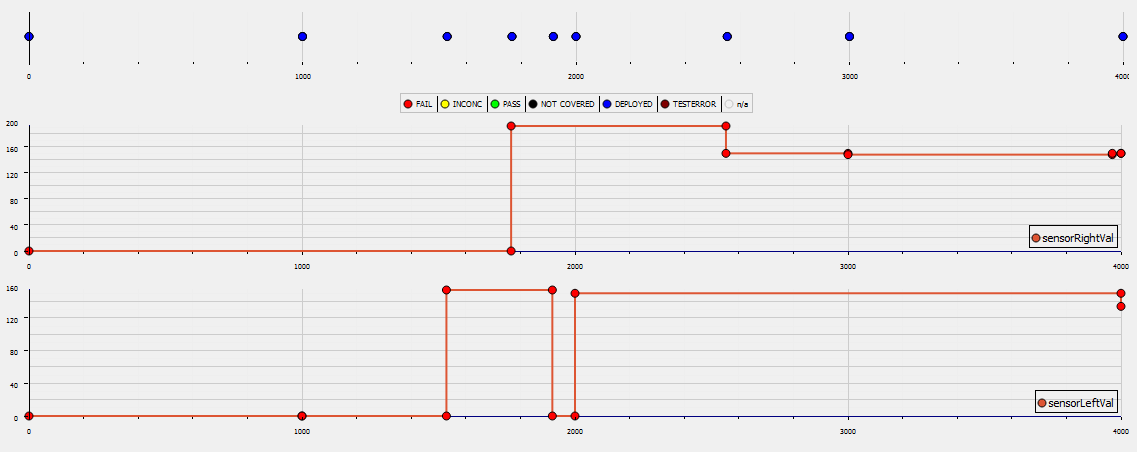
\includegraphics[width=1.0\textwidth]{lfr_input_seq}
    \caption{Test Input Sequence of LFR}
    \label{fig:lfr_test_seq}
\end{figure}

Firstly, the test result of \T{TP} against \T{Simulation} is displayed in Figure~\ref{fig:lfr_testcase_sum_sim}. All test cases should be \T{PASS} or \T{INCONCLUSIVE} because both \T{TP} and \T{Simulation} are test procedures generated from the exactly same test mode. However, three \T{FAIL}s are seen from the figure. This is because there is a very small delay in arrival time of inputs between \T{TP} and \T{Simulation}. For instance, $sensorLeftVal$ is changed to 150 from 0 at 2000 ms (as shown in Figure~\ref{fig:lfr_test_seq}) which is the time for \T{TP} to output it to \T{Simulation} as well as check of expected behaviour. But the actual time when \T{Simulation} gets the latest value 150 would be later (provided the Co-Simulation step is 1ms, and then there is 1ms delay). Finally, at 2000 ms, \T{TP} uses 150 to calculate the expected behaviour but \T{Simulation} still uses the old value 0 for $sensorLeftVal$ to give its output, which leads to mismatch of actual outputs with expected outputs. 
\begin{figure}[htb!]
    \centering
	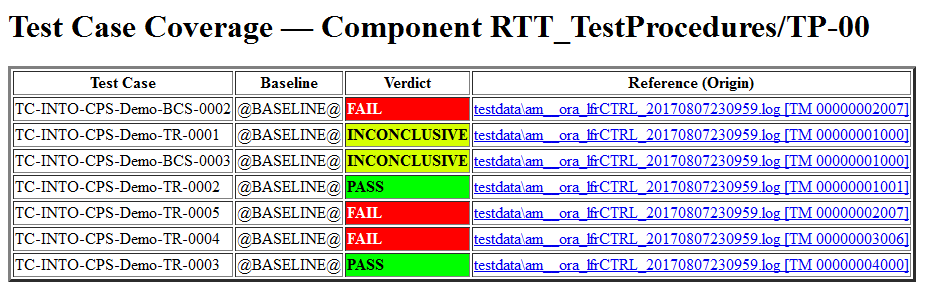
\includegraphics[width=1.0\textwidth]{lfr_sim_verdict}
    \caption{Test Case Summary (TP vs. SIM)}
    \label{fig:lfr_testcase_sum_sim}
\end{figure}

In order to correct it, we can put additional 2 ms offset manually in SUT. It is shown in the source code. Eventually, the test result of \T{TP} against \T{SUT} is displayed in Figure~\ref{fig:lfr_testcase_sum_sut} in which all test cases are \T{PASS} or \T{INCONCLUSIVE}.
\begin{figure}[htb!]
    \centering
	\includegraphics[width=1.0\textwidth]{lfr_sut_verdict}
    \caption{Test Case Summary (TP vs. SUT)}
    \label{fig:lfr_testcase_sum_sut}
\end{figure}

\subsubsection{Code Generation}

The VDM-RT model, \textbf{LFRController}, can be exported from Overture as a C code FMU, in addition to the tool wrapper FMU as used above. The \emph{LFRController-SourceCode.fmu} included in this pilot is obtained directly from Overture using the ``Export Source Code FMU'' option. However, this FMU does not contain binaries for co-simulation and so one may use the \emph{FMU Builder} included in the INTO-CPS Application to compile FMUs for Windows, Mac and Linux. 

This process has been performed and the resultant FMU is included in the pilot in the FMUs folder;  \emph{LFRController-Standalone.fmu}. One example experiment available is to switch this FMU for the tool wrapper version -- \emph{LFRController.fmu} -- and compare results. 

\clearpage

\section{Turn Indicator}
\label{sec:turn}

\subsection{Example Description}
\label{sec:turn_desc}

The turn indicator model discussed here is an adaption of a model originally
designed with an industrial partner from the automotive domain\footnote{The
  detailed model is described in~\cite{Peleska&11}.}. The model specifies the
behaviour of a turn indication controller, which essentially supports left and
right flashing as well as emergency flashing. The functionality is modelled
using three inputs (the voltage, the control lever and the emergency flash
button) and two outputs (the states of the left and right turn indication
lights, respectively).
The model can then be used to automatically generate
test cases for a system that shall implement the specified behaviour.
In addition, desired safety properties of the system can also be verified using
model checking.
Both these activities are performed using the RT-Tester Model-Based Test
Case Generator (RTT-MBT) \cite{VSI-mbt-man} and are described in more detail
in Deliverable D5.3a~\cite{INTOCPSD5.3a} and Deliverable D5.3c~\cite{INTOCPSD5.3c}, respectively.

A key feature of this example is that it combines several features which are
important for effective modelling of system specifications using SysML state
charts: It uses variables of different types (voltage is real-valued, the
other ones are integral), it uses hierarchical state machines and concurrent
components.

\subsection{Usage}
\label{sec:turnindicator_usage}

The example is available at \url{https://github.com/into-cps/example_turn_indication}
and can be downloaded as an example project directly from within the
INTO-CPS application. After that, the example can be used for test automation
and model checking activities.

In addition the \emph{VSI tools} release bundle installs a pre-configured RT-Tester project
in the directory \path{C:\Users\<USER>\RTT-Prj\turn-ind\}. The sub-folder \path{sut\}
contains a C~implementation of the system under test. The associated FMU
\path{RTT\_TestProcedures\SUT\TurnIndicationController_sut.fmu} can be run in co-simulated
test run against a generated test driver.


\subsection{SysML}
The model has been developed in Modelio by means of hierarchic parallel state-charts.
Furthermore, architecture diagrams are used to structure components and
ports, and connections are used to express data flow between parallel components.

Figure~\ref{figure:turnindicator:toplevel-achitecture} depicts the structure of
the overall \texttt{System}  which is decomposed in a
\texttt{SystemUnderTest} and a \texttt{TestEnvironment} component.
\begin{figure}[hpt!]
\centerline{\includegraphics[scale=0.5]{turnindicator/VSI-modelio_turn_indication_small_toplevel_architecture_diagram}}
\caption{Top-level architecture diagram of the turn indicator model.}
\label{figure:turnindicator:toplevel-achitecture}
\end{figure}
The \texttt{SystemUnderTest} encompasses the desired behaviour of the system under test
and has therefore been annotated with the \emph{SUT} stereotype.
The \texttt{TestEnvironment} represents the operational environment to the system under test
and is annotated with the \emph{TE} stereotype.

The system under test receives inputs from the environment and provides outputs.
For both of these, data flow interfaces specify the involved variables
and have been associated with the stereotypes \emph{SUT2TE} and \emph{TE2SUT},
respectively.
The system under test receives the following inputs from the environment:
\begin{itemize}
    \item \texttt{TurnIndLvr}: The position of the turn indicator lever, which can either be
      neutral, left flashing, or right flashing.
    \item \texttt{EmerSwitch}: The on/off status of the emergency flashing switch.
    \item \texttt{voltage}: The voltage of the car's battery.
\end{itemize}
The \texttt{SystemUnderTest} produces the following observable outputs:
\begin{itemize}
    \item \texttt{LampsLeft}: The of/off status of the indication lights on the left side.
    \item \texttt{LampsRight}: The of/off status of the indication lights on the right side.
\end{itemize}
The connection diagram in Figure~\ref{figure:turnindicator:toplevel-connections} connects
the system under test with the test environment using the described interfaces.
\begin{figure}[hpt!]
    \centerline{\includegraphics[scale=0.5]{turnindicator/VSI-modelio_turn_indication_small_toplevel_connection_diagram}}
    \caption{Top-level connection diagram of the turn indicator model.}
    \label{figure:turnindicator:toplevel-connections}
\end{figure}

Note, that the correct stereotype annotations of the components are
important for test case generation using RTT-MBT.

In this example, the {\tt TestEnvironment} does not constrain the input
variables in any way (RTT-MBT automatically ensures that the values assigned
during test case generation are within the specified range). The relevant
logic is thus implemented in {\tt SystemUnderTest}, which is divided into two
hierarchical state charts called {\tt FLASH\_CTRL} and {\tt OUTPUT\_CTRL}
as expressed by the class diagram in Figure~\ref{figure:turnindicator:sut-architecture}.
\begin{figure}[hpt!]
    \centerline{\includegraphics[scale=0.4]{turnindicator/VSI-modelio_turn_indication_small_sut_architecture_diagram}}
    \caption{System under test architecture diagram of the turn indicator model.}
    \label{figure:turnindicator:sut-architecture}
\end{figure}
The component {\tt FLASH\_CTRL} is responsible for deciding whether the left or the
right side has to flash depending on the turn-indicator lever and the emergency switch.
This general decision for the two sides is fed into the {\tt OUTPUT\_CTRL}
which is responsible for periodically turning the lights on and off.
This data flow between the two components is expressed by the connection diagram in
Figure~\ref{figure:turnindicator:sut-connections}.
\begin{figure}[hpt!]
    \centerline{\includegraphics[scale=0.5]{turnindicator/VSI-modelio_turn_indication_small_sut_connection_diagram}}
    \caption{System under test connection diagram of the turn indicator model.}
    \label{figure:turnindicator:sut-connections}
\end{figure}

The {\tt FLASH\_CTRL} state machine in Figure~\ref{figure:vsi-flash-ctrl} controls
the impact of operating the turn indicator
and emergency flashing switch. If the emergency switch is not pressed, the state machine
simply enables flashing on a specific side if the turn indicator lever is in the respective
position.
\begin{figure}[hpt!]
    \centerline{\includegraphics[scale=0.3]{turnindicator/AS_SAMPLE_FLASH_CTRL.png}}
    \caption{The {\tt FLASH\_CTRL} state machine.}
    \label{figure:vsi-flash-ctrl}
\end{figure}
If the emergency switch is pressed, the composite state in Figure~\ref{figure:vsi-emer-on}
decides whether both sides should flash. Observe, that using the turn indicator lever
while the emergency switch is pressed can override emergency flashing.
The lamps resume flashing on both sides when the turn indicator level is returned to
the neutral position.
\begin{figure}[hpt!]
    \centerline{\includegraphics[scale=0.3]{turnindicator/AS_SAMPLE_EMER_ON.png}}
    \caption{The {\tt EMER\_ON} composite state in the {\tt FLASH\_CTRL} state machine.}
    \label{figure:vsi-emer-on}
\end{figure}

{\tt OUTPUT\_CTRL} depicted in Figure~\ref{figure:vsi-output-ctrl} implements two
modes for setting the outputs. It can be in either idle or flashing mode, 
where the flashing mode itself is implemented as composite state that can
switch from off to on and vice versa. It does so in a regular interval if
the system has enough power and a lever or the emergency button has been used.
The state machine also implements a counter that ensures that left or right flashing
is still flashing for three times if the turn indicator level is only operated for a short duration.
\begin{figure}[hpt!]
    \centerline{\includegraphics[scale=0.3]{turnindicator/AS_SAMPLE_OUTPUT_CTRL.png}}
    \caption{The {\tt OUTPUT\_CTRL} state machine.}
    \label{figure:vsi-output-ctrl}
\end{figure}

Observe that certain states and transitions in the model have been
annotated with requirements. For example, the transition from state ${\tt
TURN\_IND\_OVERRIDE} \to {\tt EMER\_ACTIVE}$ in
Figure~\ref{figure:vsi-emer-on} has been linked to requirement {\sf REQ-007}
via a \emph{satisfy relation}. Likewise, state {\tt TURN\_IND\_OVERRIDE} has
been linked to requirement {\sf REQ-006}.
Linking requirements in that way specifies that the associated structural elements
of the model help to realise the given requirement.

Furthermore, some requirements are attached to classes in conjunction with an LTL formula
as can be seen in Figure~\ref{figure:turnindicator:sut-architecture}.
The LTL formula specifies an abstract execution trace that could serve as a witness
to demonstrate that the requirement is fulfilled by an implementation.

\subsection{Analyses and Experiments}

\subsubsection{Test Automation and Model Checking}
As mentioned earlier, this pilot can be used to automatically generate
test cases for a system that shall implement the specified behaviour.
In addition, desired safety properties of the system can also be verified using
model checking.
Both these activities are performed using the RT-Tester Model-Based Test
Case Generator (RTT-MBT) and are described in more detail
in Deliverable D5.3a~\cite{INTOCPSD5.3a} and Deliverable D5.3c~\cite{INTOCPSD5.3c}, respectively.

\clearpage
%!TEX root = ../D3.5_Examples_Compendium_2.tex
\section{Unmanned Aerial Vehicle}
\label{sec:uavsingle}
This example is no longer maintained or updated. You are welcome to contact the example owner in case of interest.
See \url{https://github.com/INTO-CPS-Association/example-single_uav} for contact details.

	\subsection{Example Description}
	\label{sec:uavsingle_desc}
		This pilot study originates from a master thesis study presented in \cite{Grujic&16}.
		The study models the physical dynamics as well as the discrete controller of an Unmanned Aerial Vehicle (UAV).
		Focus on the details of the model contribute to a high model fidelity, enabling the multi-model to be used to compare alternative control algorithms.

		\autoref{fig:uav_3d_model} shows a 3D model of the UAV and some of its main components, including the \texttt{airframe}, which is the main body the UAV, the propulsion system consisting of \texttt{rotors}, \texttt{motors}, and \texttt{electronic speed controllers}, along with the \texttt{battery} and the \texttt{controller} platform.
		Additionally, a UAV have a range of different \texttt{sensors} and a \texttt{telemetry system} used to communicate with a pilot or a ground control center.

		\begin{figure}[htbp]
			\centering
			\includegraphics[width=0.7\linewidth]{uavsingle/drone.pdf}
			\caption{UAV 3D model}
			\label{fig:uav_3d_model}
		\end{figure}

	\subsection{Usage}
	\label{sec:uavsingle_usage}
		The example is available at \url{https://github.com/INTO-CPS-Association/example-single_uav} in the \emph{master} branch. There are several subfolders for the various elements: \texttt{FMU} -- contains the various FMUs of the study; \texttt{Models} -- contains the constituent models defined using the INTO-CPS simulation technologies; \texttt{Multi-models} -- contains the multi-model definitions and co-simulation configurations -- with 3D and non-3D options; and \texttt{SysML} -- contains the SysML model defined for the study.

		In the \emph{abstract\_intocps} branch, the original discrete event control model have been replaced with an abstract control model in order to enable high-level control prototyping.
		A prototype of an autonomous vertical waypoint controller is exemplified.
		The same model is found in the \emph{abstract\_crescendo} branch, where DESTECS technology is used instead of INTO-CPS technology.
		This can be used to compare the two technologies \cite{Thule&16b}.

	\subsection{INTO-CPS SysML profile}
	\label{sec:uavsingle_into_sys}
		The INTO-CPS SysML profile is used to create an Architecture Structure Diagram (ASD) and a Connections Diagram (CD), shown in \autoref{fig:uav_architecture_diagram} and \autoref{fig:uav_connections_diagram} respectively.
		The ASD expresses that the system \texttt{UAV} is a composition of a cyber part \texttt{ArduPilot}, a physical part \texttt{ArduCopter}, and an optional \texttt{3D animation}.

		\texttt{ArduPilot} is a discrete event controller described in VDM-RT. 
		It takes a number of sensor inputs and outputs a control signal for each of the four motors of the UAV.
		By adjusting the motor setpoints, it is able to make the UAV fly to predefined waypoints, taking into account feedback from sensors.

		\texttt{ArduCopter} is a model of the physical dynamics of the UAV described in 20-sim.
		The inputs to the \texttt{ArduCopter} model are the four motor setpoints. 
		Based on these, it calculates the angular position described with roll, pitch, and yaw angles, and the spatial position described with a latitude, longitude, and altitude (X,Y,Z), and the velocities and accelerations of the UAV.
		Additionally, corresponding sensor outputs are simulated for a 3-axis accelerometer, a 3-axis gyroscope and a GPS. 
		
		Angular and spatial positions are used by the \texttt{3D animation}.

		\begin{figure}[htbp]
			\centering
			\includegraphics[width=\linewidth]{uavsingle/architecture_diagram.png}
			\caption{UAV Architecture Structure Diagram}
			\label{fig:uav_architecture_diagram}
		\end{figure}

		The connection between the constituent models is a one-to-one mapping between \texttt{ArduPilot} and \texttt{ArduCopter}, with the exception that the \texttt{3D animation} is connected to \texttt{ArduCopter} as well, as shown in \autoref{fig:uav_connections_diagram}.
		

		\begin{figure}[htbp]
			\centering
			\includegraphics[width=\linewidth]{uavsingle/connections_diagram_3d.png}
			\caption{UAV Connections Diagram}
			\label{fig:uav_connections_diagram}
		\end{figure}


	\subsection{Multi-model}
	\label{sec:uavsingle_into_mm}

	\subsubsection{Models}
		The system comprises a continuous-time (CT) model \texttt{ArduCopter} and a discrete event (DE) model \texttt{ArduPilot}.
		\begin{description}
			\item[ArduCopter:] 
				The physical dynamics of the UAV is described in 20-sim.
				In \autoref{fig:uav_20-sim_model} an overview of the \texttt{Quadcopter} model is shown.
				It includes the rigid body dynamics of the \texttt{airframe}, the aerodynamics of the \texttt{rotors}, the electronics and mechanics of the \texttt{motors} and the \texttt{electronic speed controllers}, as well as \texttt{sensor} noise, inaccuracies, and rounding errors. 
				\begin{figure}[htbp]
					\centering
					\includegraphics[width=\linewidth]{uavsingle/ct_model.png}
					\caption{20-sim model of the UAV}
					\label{fig:uav_20-sim_model}
				\end{figure}

			\item[ArduPilot:]
				\autoref{fig:uav_ardupilot_overview} shows an overview of the \texttt{ArduPilot} model, which is described in VDM-RT.
				The main class of the model \texttt{ArduPilot} starts a \texttt{Scheduler} and a \texttt{Flight controller}.
				To improve model fidelity, sensor values are updated periodically by the scheduler to emulate the real update frequencies of the various sensors.
				The flight controller takes input from a pilot and from sensor data, on which sensor fusion is performed, and is responsible for calculating desired accelerations for the UAV. 
				These accelerations are translated, by the \texttt{Motors} class, into motor setpoints for each motor.
				The translation involves a complex tradeoff between roll, pitch, and yaw accelerations and total thrust.
				The \texttt{MotorsQuad} class is shown to illustrate that the \texttt{Motors} class can be extended to support any number or configuration of motors.

				The \texttt{Flight Control} class contains the core functionality of the model and is probably also the most complex part.
				It can operate in multiple flight modes, which make use of either an attitude controller or both an attitude and a position controller.
				The attitude controller is capable of obtaining and maintaining any given attitude, whereas the position controller is capable of controlling the altitude.
				Both the attitude and position controllers depend on a number of low level controllers, such as Proportional-Integral-Derivative (PID) controllers and a number of different filters to remove unwanted noise and vibrations caused by the fast spinning rotors.
				\begin{figure}[htbp]
					\centering
					\includegraphics[width=\linewidth]{uavsingle/detailed_de_model.png}
					\caption{ArduPilot model overview}
					\label{fig:uav_ardupilot_overview}
				\end{figure}

		\end{description}
		
	\subsubsection{Configuration}
		This pilot study does not use any parameters and the connections should be self explanatory from \autoref{fig:uav_connections_diagram}.

	\subsection{Co-simulation}
	\label{sec:uavsingle_into_co}
		Two multi-models are defined for this pilot study.
		The only difference between the two is whether the 3D animation is included or not.

		\begin{figure}[htbp]
			\centering
			\includegraphics[width=0.5\linewidth]{uavsingle/drone_animation_cropped.png}
			\caption{3D visualization of the UAV}
			\label{fig:uav_3d_animation}
		\end{figure}
%%% Local Variables:
%%% mode: latex
%%% TeX-master: "../INTO-CPS_Examples_Compendium"
%%% End:

\clearpage
\section{Ether}
\label{sec:ether}
%\fbox{Responsible: UNEW, Provisional date: Nov 2016}

\subsection{Example Description}
\label{sec:ether_desc}

This example explores ways to model network communications between controllers. This involves passing messages ---VDM values encoded as strings--- from a model called \emph{Sender} to a model called \emph{Receiver}. This is either done directly, as illustrated in Figure~\ref{fig:send_rec}, or via a third model called the \emph{Ether}, as illustrated in Figure~\ref{fig:send_ether_rec}.

While this example demonstrates that direct connection is possible, for multi-models with large numbers of connected controllers (for example swarms or cooperative vehicles) it becomes unwieldy. This example includes an Ether model, which represents an abstract communication mechanism, that handles message passing between the Sender and Receiver. This Ether can be used in other models.

The introduction of a model of communications also permits a range of realistic and faulty behaviours to be introduced, such as message delay, duplication, and loss. The ether pattern which this example implements is described in greater detail in Deliverable D3.3a~\cite{INTOCPSD3.3a}, and includes a discussion of realistic and faulty behaviour.

\begin{figure}[h]
\begin{center}
\subfigure[Sender and Receiver connected directly]
{
     \includegraphics[scale=0.5]{ether/send_rec}
      \label{fig:send_rec}
}
\hspace{2em}\subfigure[Sender and Receiver connected via the Ether]
{
     \includegraphics[scale=0.5]{ether/send_ether_rec}
      \label{fig:send_ether_rec}
}
\caption{Topology of the `Direct' and `Ether' multi-models.}
\label{fig:ether_topology}
\end{center}
\end{figure}

\subsection{Usage}
\label{sec:ether_usage}

The example is available from the INTO-CPS application menu at \emph{File > Import Example Project} or at  \url{https://github.com/INTO-CPS-Association/example-ether} in the \emph{master} branch. There are several subfolders for the various elements: \texttt{FMU} -- contains the various FMUs of the study; \texttt{Models} -- contains the constituent models defined using the INTO-CPS simulation technologies; \texttt{Multi-models} -- contains the multi-model definitions and co-simulation configurations -- with Direct and Ether configurations.

The \texttt{case-study\_ether folder} can be opened in the INTO-CPS application to run various co-simulation experiments. To run a simulation, expand the emph{Direct} or emph{Ether} models, then open the \emph{co-sim\_direct} or {co-sim\_ether} experiments and click \emph{Simulate}. Section~\ref{sec:ether_into_analysis} below gives some suggestions of how to explore the multi-model.

%\textbf{Warning!} Values printed from Overture FMUs are not visible in the COE status window in the INTO-CPS Application version 2.1.0 or below.

%\subsection{INTO-CPS Technology}
%\label{sec:ether_into}

%\subsection{INTO-CPS SysML profile}
%\label{sec:ether_into_sys}

\subsection{Multi-model}
\label{sec:ether_into_mm}

\subsubsection{Models}

There are three models in this example, all of which are DE models written in VDM:

\begin{description}
  \item[Sender:] This model has a single output port called \texttt{out}, of type \texttt{String}. The \texttt{Controller} class generates random messages every 0.1 seconds, and passes them to the output port. Each message consists of three integers in the range (0,10), and are converted to a string representation using the \texttt{VDMUtil} standard library. The time and content of each message is printed to the console.
  \item[Receiver:] This model has a single input port called \texttt{iin}, of type \texttt{String}. The \texttt{Controller} class listens for messages on the input port and attempts to convert message strings back to a VDM type representation using the \texttt{VDMUtil} standard library. Empty strings are often received at the start of co-simulation, and these are ignored. If conversion is successful, the time and content of the message is printed to the console.
  \item[Ether:] This model represents an abstract communication medium. It has an input port called \texttt{sender} and an output port called \texttt{receiver}, both of type \texttt{String}. The \texttt{Ether} class passed strings from the \texttt{sender} port to the \texttt{receiver} port. Although in this example only one message will be received at a time, in general there may be multiple messages for the same destination during a single update, so the \texttt{Ether} class collects messages in a list and passes on a string of strings that the destination (i.e.\ in this case Receiver) must decode.

      The connections in the \texttt{Ether} class are determined by the values passed to the constructor, which is called in the \texttt{System} class. The constructor takes a map of named input ports, a map of named output ports and a set of pairs indicating which inputs are connected to which outputs. The \texttt{Ether} class does not examine the value of the messages that it passes. This model can be reused in other multi-models where message-based communications between models are required.
\end{description}

\subsubsection{Configuration}

There are two multi-model configurations included in the example:

\begin{description}
  \item[Direct] In this configuration, the \texttt{Sender.out} port is connected directly to the \texttt{Receiver.in} port.
  \item[Ether] In this configuration, the \texttt{Sender.out} port is connected to the \texttt{Ether.sender} port and the \texttt{Sender.reciever} port is connected to the \texttt{Receiver.in} port.
\end{description}

These two different configurations allow exploration of the consequences of introducing the Ether FMU. The Sender model does not need to know if it is connected to the Ether or not. Since the Ether allows one-to-many communications, it passes lists of values, so the Receiver must check whether it received a single value from the Sender directly, or a list containing a single value via the Ether. This could be avoided in this example by letting the Ether assume that there is only one connection, but would make the Ether less general. The included implementation means that the Ether can be used directly in other multi-models --- only the \texttt{HardwareInterface} class and called to the constructor of \texttt{Ether} would need to be changed for the context of the new model.

\subsection{Co-simulation}
\label{sec:ether_into_co}

The simulation time for the multi-model is set to one second, which is sufficient to see the behaviour of the system. During this time, 10 messages are sent from the Sender.  Not all messages are received by the Receiver since at least one extra update cycle is needed to process the final message, or final two messages in the case of communication via the Ether.

\subsection{Analyses and Experiments}
\label{sec:ether_into_analysis}


\subsubsection{Sample Experiments}
\label{sec:ether_exp}

The following experiments are instructive in demonstrating the effects on introducing the Ether and the effects of the relative speeds up the \emph{Sender}, \emph{Ether} and \emph{Receiver} on messages. All three FMUs print messages and times to the COE console.

\begin{enumerate}
  \item Run the \emph{Direct} co-simulation and observe that messages arrive at Receiver one step (0.1 seconds) later. Run the \emph{Ether} co-simulation and observe that messages arrive two steps (0.2 seconds) later.
  \item Change the frequency of the Ether to 20Hz or higher. Run the \emph{Ether} co-simulation and observe that messages arrive at Receiver one step (0.1 seconds) later. This is because the Ether can now update in between steps of the Receiver.
  \item Set the Ether back to 10Hz and change the frequency of the Sender to 20Hz or higher. Run the \emph{Ether} co-simulation and note how messages are not lost because they are changed by the Sender before they are read by the Ether.
  \item Set the Sender back to 10Hz and change the frequency of the Receiver to 20Hz or higher. Run the \emph{Ether} co-simulation and note how messages are now duplicated because the Receiver is reading them twice or more.
\end{enumerate}

If elimination of message loss or duplication is important in a multi-model,
the description of the ether pattern in Deliverable D3.3a~\cite{INTOCPSD3.3a} gives some initial guidance on overcoming such problems by introducing extra logic to give quality of service (QoS) guarantees in message-passing. 


\subsubsection{Test Automation and Model Checking}
\label{sec:ether_ta}
\graphicspath{ {./ether/TA/} }

Our model for test automation is different from that for Multi-model and analysis in the following aspects.
\begin{itemize}
    \item Our test model aims for model network communications between multiple controllers through an intermediate \emph{Ether}. The \emph{Ether} is regarded as a shared medium between controllers to dispatch packages from multiple sources to multiple targets. Therefore, we do not need all controllers connected to each other directly and the direct connection mode between controllers is not taken into account in our test model.
    \item Current Multi-model configuration \B{Ether} includes only one \T{Sender} and one \T{Receiver}. In order to be used as a communication medium in the UAV swarm pilot study in Section~\ref{sec:uavswarm}, the \emph{Ether} model should support more senders and receivers. Our test model supports two controllers to be connected through the \emph{Ether}, and each controller is composed of a sender and a receiver to allow it to communicate with others bidirectionally.
    \item For Co-Simulation, these controllers could be in different FMUs. Then the \emph{Ether} should provide the capability to dispatch packages from sources to destinations according to their targets. For instance, one central controller would send a command to the controller one at a specific time, then later it would send another command to the controller two. We introduce a new package structure (as shown in Section~\ref{sssec:ether_encoding}) which is composed of an address part and a payload part. Therefore, the \emph{Ether} is able to dispatch packages by the addresses that are encoded in the packages. In particular, it supports broadcast and unicast.
    \item The model for Multi-model and analysis has messages encoded in strings. But due to the fact that RT-Tester is not able to parse string or array in test models, we are not able to model variable-length strings in test models. The encoding mechanism in Section~\ref{sssec:ether_encoding} is an example to encode a string (up to 5 Base64 characters) into a 32-bit integer. We allow different applications can have different encoding mechanisms. As an example, the test model in the UAV swarm study uses three doubles for its payload and each double means a position or velocity in one of three axes (X, Y and Z). However, for this \emph{Ether} pilot study, the test model will not look into the inside of payloads and it just uses an integer for illustration.
\end{itemize}

Subsequently, we present the test model in SysML. Then model checking is applied to check a number of properties of the test model. Finally a SUT is implemented manually and test automation is applied to test whether the SUT is a correct implementation of the test model.

\paragraph{Test Model [Ether mode]}
Our test model connected two controllers (or FMUs, here we call it \emph{End}) through a \emph{Ether}. The interfaces between the \emph{TestEnvironment} and the \emph{SystemUnderTest} are the packages that two \emph{Ends} would send and receive.

\subparagraph{String Encoding}
\label{sssec:ether_encoding}
A package is composed of two parts: address and payload. Each of them is encoded in one integer (32-bit). 
\begin{itemize}
    \item Address (32-bit integer): the high 24 bits are always 0, the low 8 bits are split into two 4-bit parts (one for the destination port and one for the source port)
        \begin{itemize}
            \item 0xF: for broadcast;
            \item 0x1-0xE: port 1 - port 15;
            \item 0x0: no message signal (used for the polling method to identify a valid package).
        \end{itemize}
    \item Payload (32-bit integer): the highest two bits are reserved, other 30 bits consist of five 6-bit parts (each encodes a Base64 character)
        \begin{itemize}
            \item Base64: 64 characters (26 uppercase alphabet letters [A-Z], 26 lowercase alphabet letters [a-z], 10 digits [0-9], '+' and '/'),
            \item up to five characters in a string.
        \end{itemize}
\end{itemize}

Finally, it supports
\begin{itemize}
    \item up to 15 incoming ports and 15 outgoing ports, and each FMU (or end) has a paired incoming and outgoing ports,
    \item up to 15 FMUs connected,
    \item the paired ports have the same and unique id,
    \item the destination address of an input pair can be its paired port (send a message to itself),
    \item up to 5 characters in the payload of each package.
\end{itemize}

\subparagraph{Inputs and Outputs}
Inputs and outputs of the test model are shown in Figure~\ref{fig:ether-inouts}.
\begin{figure}[htb!]
    \centering
    \includegraphics[width=0.4\textwidth]{ether_inouts}
    \caption{Input and Output Variables of Ether}
    \label{fig:ether-inouts}
\end{figure}

The \emph{SystemUnderTest} receives the following inputs (stimuli) from the \emph{TestEnvironment}:
\begin{itemize}
    \item $in1a$ and $in1p$: address and payload of the incoming package in \emph{Ether} from End 1, 
    \item $in2a$ and $in2p$: address and payload of the incoming package in \emph{Ether} from End 2. 
\end{itemize}

The \emph{SystemUnderTest} provides the following observable outputs to the \emph{TestEnvironment}:
\begin{itemize}
    \item $out11a$ and $out11p$: address and payload of the first outgoing package in \emph{Ether} to End 1,
    \item $out12a$ and $out12p$: address and payload of the second outgoing package in \emph{Ether} to End 1,
    \item $out13a$ and $out13p$: address and payload of the third outgoing package in \emph{Ether} to End 1,
    \item $out21a$ and $out21p$: address and payload of the first outgoing package in \emph{Ether} to End 2,
    \item $out22a$ and $out22p$: address and payload of the second outgoing package in \emph{Ether} to End 2,
    \item $out23a$ and $out23p$: address and payload of the third outgoing package in \emph{Ether} to End 2. 
\end{itemize}

\subparagraph{Other Interfaces}
Other interfaces, as shown in Figure~\ref{fig:ether-other-ifs}, are used in the \emph{SystemUnderTest} for connections between the \emph{Ends} and the \emph{Ether}.
\begin{figure}[htb!]
    \centering
    \includegraphics[width=0.4\textwidth]{ether_other_ifs}
    \caption{Other Interfaces of Ether}
    \label{fig:ether-other-ifs}
\end{figure}

\begin{itemize}
    \item $InMsgIF$ and $OutMsgIF$: the incoming and outgoing interfaces between the \emph{End1} and the \emph{Ether}, 
    \item $InMsgIF2$ and $OutMsgIF2$: the incoming and outgoing interfaces between the \emph{End2} and the \emph{Ether}.
\end{itemize}

\subparagraph{SystemUnderTest Architecture Diagram}
The system architecture diagram of the \emph{SystemUnderTest} is shown in Figure~\ref{fig:ether-sut-sad}. It consists of two \emph{Ends}: \emph{End1} and \emph{End2}, and one \emph{Ether}.
\begin{figure}[htb!]
    \centering
    \includegraphics[width=0.7\textwidth]{ether_sut_sad}
    \caption{Ether Architecture Diagram}
    \label{fig:ether-sut-sad}
\end{figure}

\subparagraph{SystemUnderTest Connection Diagram}
The connection diagram of the \emph{SystemUnderTest} is illustrated in Fig~\ref{fig:ether-cd}. Both \emph{End1} and \emph{End2} are connected to the \emph{Ether}, but they are not connected directly. Therefore, a package that is sent from the \emph{End1} to the \emph{End2} would transmit to the \emph{Ether} at first, then dispatch to the \emph{End2} by the \emph{Ether}. 

\begin{figure}[htb!]
    \centering
    \includegraphics[width=0.8\textwidth]{ether_sut_cd}
    \caption{Ether Connection Diagram}
    \label{fig:ether-cd}
\end{figure}

\subparagraph{End1 State Machine Diagram}
The behaviour of the \emph{End1} is specified in the state machine diagram shown in Figure~\ref{fig:ether-sut-end1-sm}. It merely copies the input packages from the \emph{TestEnvironment} to the \emph{Ether} and the output packages from the \emph{Ether} to the \emph{TestEnvironment}.

\begin{figure}[htb!]
    \centering
	\includegraphics[width=0.7\textwidth]{ether_sut_end1_sm}
    \caption{End1 State Machine Diagram}
    \label{fig:ether-sut-end1-sm}
\end{figure}

\subparagraph{End2 State Machine Diagram}
Similarly, the state machine diagram of the \emph{End2} is displayed in Figure~\ref{fig:ether-sut-end2-sm}.

\begin{figure}[htb!]
    \centering
	\includegraphics[width=0.8\textwidth]{ether_sut_end2_sm}
    \caption{End2 State Machine Diagram}
    \label{fig:ether-sut-end2-sm}
\end{figure}

\subparagraph{Ether State Machine Diagram}
The behaviour of the \emph{Ether} is specified in the state machine diagram shown in Figur~\ref{fig:ether-sut-ether-sm}. Basically, it checks the incoming packages from the \emph{End1} and the \emph{End2}, and then dispatches them to their corresponding output ends according to the address in each package.

\begin{figure}[htb!]
    \centering
	\includegraphics[width=1.0\textwidth]{ether_sut_ether_sm}
    \caption{Ether State Machine Diagram}
    \label{fig:ether-sut-ether-sm}
\end{figure}

\subparagraph{Test Input Simulation} We use a state machine to specify the input sequence in the \T{TestEnvironment} of the test model. The diagram is shown in Figure~\ref{fig:ether-te-sim-sm}. This state machine simulates all combinations of incoming packages from the \emph{End1} and \emph{End2} in terms of package addresses. 

\begin{figure}[htb!]
    \centering
	\includegraphics[width=1.0\textwidth]{ether_te_sim_sm}
    \caption{Test Input Simulation State Machine Diagram}
    \label{fig:ether-te-sim-sm}
\end{figure}

\paragraph{Model Checking}

Model checking can be applied to the test model to check if it satisfies several properties. In order to use bounded model checking in the INTO-CPS app, we set the bounded steps ``BMC steps'' to 50. The properties below are checked to hold in 50 steps.

\begin{description}
    \item[P0] Livelock property by the \B{Check Mode} function on RT-Tester.
\begin{verbatim}
Check static model semantics ...done.
- IMR.SystemUnderTest.End1I... [PASS]
- IMR.SystemUnderTest.End2I... [PASS]
- IMR.SystemUnderTest.EtherI... [PASS]
- IMR.TestEnvironment.tesimulator... [PASS]
\end{verbatim}

    \item[P1] An \emph{End} would never receive a package with a wrong destination address.
\begin{verbatim}
Globally ([IMR.out11a != 33] && 
    [IMR.out11a != 34] && 
    [IMR.out21a != 17] && 
    [IMR.out21a != 18])
\end{verbatim}

    \item[P2] All controllers could be in the \emph{Idle} state at the same time.
\begin{verbatim}
Finally ([IMR.SystemUnderTest.End1I.End.Idle
    && IMR.SystemUnderTest.EtherI.Ether.Idle
    && IMR.SystemUnderTest.End2I.End.Idle])
\end{verbatim}

    \item[P3] A broadcast package would never be received by its source port.
\begin{verbatim}
Globally ([IMR.out11a != 241] && [IMR.out21a != 242])
\end{verbatim}
\end{description}

\paragraph{A Manual Implementation of SUT in C}
A SUT is implemented in C. And it is finally built and wrapped into a SUT FMU.

\paragraph{Test Results}

\subparagraph{Test Goals}
Our test goals configuration is displayed in Figure~\ref{fig:ether-ta-tr01-testgoal}. All basic control state coverage test cases and transition coverage test cases for three controllers are included, in the context of the \emph{TestEnvironment} simulation enabled. In addition, a user defined test case is presented to require the test lasting at least 1.5 seconds. The generated and solved input signals for the test goals are shown in Figure~\ref{fig:ether-ta-tr01-signal-inputs-tp1} and Figure~\ref{fig:ether-ta-tr01-signal-inputs-tp2}.

\begin{figure}[htb!]
	\centering
	\includegraphics[width=1.0\textwidth]{tr01/tr01-testgoals}
	\caption{Test Goals Configuration}
	\label{fig:ether-ta-tr01-testgoal}
\end{figure}

\begin{figure}[htb!]
    \centering
	\includegraphics[width=1.0\textwidth]{tr01/tr01-signal-inputs-tp1}
    \caption{Input Signals of \emph{End1}}
    \label{fig:ether-ta-tr01-signal-inputs-tp1}
\end{figure}

\begin{figure}[htb!]
    \centering
	\includegraphics[width=1.0\textwidth]{tr01/tr01-signal-inputs-tp2}
    \caption{Input Signals of \emph{End2}}
    \label{fig:ether-ta-tr01-signal-inputs-tp2}
\end{figure}

The input address signals for both \emph{End1} and \emph{End2} (where the payloads are excluded) are marked and illustrated in Figure~\ref{fig:ether-ta-tr01-signal-inputs}.

\begin{figure}[htb!]
    \centering
	\includegraphics[width=1.0\textwidth]{tr01/tr01-signal-inputs}
    \caption{Input Address Signals}
    \label{fig:ether-ta-tr01-signal-inputs}
\end{figure}

\subparagraph{\emph{TP-00} vs. \emph{Simulation}}
The \emph{TP-00} is a test procedure in RT-Tester that provides test inputs and checks expected results, while \emph{Simulation} is a SUT test procedure created from the same test model as the \emph{TP-00}. Our test results show all these test cases are with \T{PASS} or \T{INCONCLUSIVE} verdicts. 

\subparagraph{\emph{TP-00} vs. \emph{SUT}}
This is to test if our manually implemented SUT is a correct implementation of the test model or not. Our test results show all these test cases are with \T{PASS} or \T{INCONCLUSIVE} verdicts. Corresponding to the inputs shown in Figure~\ref{fig:ether-ta-tr01-signal-inputs-tp1} and Figure~\ref{fig:ether-ta-tr01-signal-inputs-tp2} as well as the marked input signals in Figure~\ref{fig:ether-ta-tr01-signal-inputs}, the output signals for the \emph{End1} and the \emph{End2} are illustrated in Figure~\ref{fig:ether-ta-tr01-signal-output-1} and Figure~\ref{fig:ether-ta-tr01-signal-output-2} respectively.

\begin{figure}[htb!]
    \centering
	\includegraphics[width=1.0\textwidth]{tr01/tr01-signal-output-1}
    \caption{Output Signals of \emph{End1}}
    \label{fig:ether-ta-tr01-signal-output-1}
\end{figure}

\begin{figure}[htb!]
    \centering
	\includegraphics[width=1.0\textwidth]{tr01/tr01-signal-output-2}
    \caption{Output Signals of \emph{End2}}
    \label{fig:ether-ta-tr01-signal-output-2}
\end{figure}

 Our test results show all these test cases are with \T{PASS} or \T{INCONCLUSIVE} verdicts. These signals are described below with numbering.
\begin{itemize}
    \item 1. Broadcast from \emph{End1} ([100ms, 200ms]), 
        \begin{itemize}
            \item as shown in the outputs of \emph{End2} ([300, 400]),
            \item therefore, 200ms delay.
        \end{itemize}
    \item 2. Broadcast from \emph{End2} ([200, 400]), 
        \begin{itemize}
            \item as shown in the outputs of \emph{End1} ([400, 600]).
        \end{itemize}
    \item 3. Broadcast from \emph{End1} ([300, 400]), 
        \begin{itemize}
            \item as shown in the outputs of \emph{End2} ([500, 600]).
        \end{itemize}
    \item 4. Unicast from \emph{End1} to \emph{End1} ([400, 600]), 
        \begin{itemize}
            \item as shown in the output (\verb+out11a+) of \emph{End1} ([600, 800]).
        \end{itemize}
    \item 5. Broacast from \emph{End2} ([500, 600]), 
        \begin{itemize}
            \item as shown in the output (\verb+out12a+) of \emph{End1} ([700, 800]).
        \end{itemize}
    \item 6. Unicast from \emph{End2} to \emph{End2} ([600, 800]), 
        \begin{itemize}
            \item as shown in the output (\verb+out21a+) of \emph{End2} ([800, 900]),
            \item and the output (\verb+out22a+) of \emph{End2} ([900, 1000]).
        \end{itemize}
    \item 7. Unicast from \emph{End1} to \emph{End2} ([700, \ldots]), 
        \begin{itemize}
            \item as shown in the output (\verb+out21a+) of \emph{End2} ([900, 1000]).
        \end{itemize}
    \item 8. Unicast from \emph{End2} to \emph{End1} ([900, 1000]), \ldots
\end{itemize}

These behaviours are expected in our test model.

\clearpage
\section{Swarm of UAV}
\label{sec:uavswarm}

\subsection{Example Description}
\label{sec:uavswarm_desc}

The Unmanned Aerial Vehicle (UAV) Swarm pilot study is concerned with a collection of UAVs that communicate in order to achieve some global behaviour. The pilot study is related to the previous UAV study in Section~\ref{sec:uavsingle}, however this does not focus on the low-level physical details. The pilot uses a simplified physical model to allow simulation of multiple UAVs simultaneously communicating.

In this pilot, each UAV is able to adjust its pitch, yaw and roll to move in 3D space using rotors. Figure~\ref{fig:single_uav} shows a single UAV with its motors, rotors and battery -- each UAV has a controller which is able to communicate with its environment. In a swarm, the UAVs may cooperate in order to avoid collide, to achieve some predefined topology, or collaborate to provide some functionality. In this study, we demonstrate the use of a central controller to dictate the desired movements of the UAVs comprising the swarm.

\begin{figure}[htbp]
\begin{center}
\includegraphics[width=0.6\textwidth]{uavswarm/uav}
\caption{UAV 3D model}
\label{fig:single_uav}
\end{center}
\end{figure}

\subsection{Usage}
\label{sec:uavswarm_usage}

The example is available from the INTO-CPS application menu at \emph{File>Import Example Project} or at  \url{https://github.com/INTO-CPS-Association/example-uav_swarm} in the \emph{master} branch. There are several subfolders for the various elements: \texttt{FMU} -- contains the various FMUs of the study; \texttt{Models} -- contains the constituent models defined using the INTO-CPS simulation technologies; \texttt{Multi-models} -- contains the multi-model definitions and co-simulation configurations -- with 3D and non-3D options; and \texttt{SysML} -- contains the SysML model defined for the study.

The \texttt{case-study\_uav\_swarm folder} can be opened in the INTO-CPS application to run various co-simulation experiments. To run a simulation, expand one of the multi-models and click `Simulate' for an experiment. 

%\subsection{INTO-CPS Technology}
%\label{sec:uavswarm_into}

\subsection{INTO-CPS SysML profile}
\label{sec:uavswarm_into_sys}

Using the INTO-SysML profile, we model a subset of the pilot study. The reason for modelling only a small subset will become clear in this section. In Figure~\ref{fig:uav_asd}, we show an Architecture Structure Diagram (ASD) depicting 3 UAVs -- each comprised of a \emph{UAVController} component and a \emph{UAV} component, a component for 3D visualisation \emph{UAV 3D}, and a \emph{UAV Global Controller} component. Each component has a large number of inputs and outputs. Briefly the \emph{UAV} has inputs for setting the pitch, yaw, roll and throttle, and outputs for the position, velocity and battery status. The \emph{UAV Controller} has the same ports, but with reversed direction and also ports to receive commands from the global controller. The optional \emph{UAV 3D} takes as input the position, pitch, yaw and roll of each UAV. Finally, the \emph{UAV Global Controller} has a collection of ports for target locations for each UAV. 

\begin{figure}[htbp]
\begin{center}
\includegraphics[width=0.95\textwidth]{uavswarm/swarm_asd}
\caption{UAV Swarm Architecture Structure Diagram}
\label{fig:uav_asd}
\end{center}
\end{figure}

Due to the large number of ports and connectors in this pilot, it is not appropriate to represent them all on the same diagram. As such, we create a single Connections Diagram (CD) per UAV each containing the same system instance (\emph{swarm : UAVSwarm}). Combining all CDs produces a complete configuration for that system instance.  The CD in Figure~\ref{fig:uav1_cd} depicts connections between the \emph{UAVController} component and a \emph{UAV} component of UAV1, and the connections to the \emph{UAV 3D} and \emph{UAV Global Controller} components related to UAV1. Note that the \emph{UAV 3D} and \emph{UAV Global Controller} instances have a subset of their ports shown.

\begin{figure}[htbp]
\begin{center}
\includegraphics[width=0.95\textwidth]{uavswarm/swarm_cd}
\caption{UAV Swarm Connections Diagram showing connections relating to UAV1}
\label{fig:uav1_cd}
\end{center}
\end{figure}


\subsection{Multi-model}
\label{sec:uavswarm_into_mm}

\subsubsection{Models}
There are three models defined here (we do not include a description of the UAV 3D model.

\begin{description}
\item[UAV:] The physical model -- \emph{UAV} is defined in 20-sim. The \emph{UAV} model represents the motors, rotors, battery and implicitly the frame of the UAV. The top-level structure of the model is shown in Figure~\ref{fig:swarm-20-sim}.

\begin{figure}[htbp]
\begin{center}
\includegraphics[width=0.9\textwidth]{uavswarm/uav-20-sim-uav}
\caption{20-sim model for UAV taking part in a Swarm}
\label{fig:swarm-20-sim}
\end{center}
\end{figure}

As can be seen from Figure~\ref{fig:swarm-20-sim}, there are several input and output signal ports -- these correspond to those ports defined in the SysML model above -- for setting the pitch, yaw and roll and reporting various aspects for control and visualisation purposes. The model is simplified and more abstract from that in Section~\ref{sec:uavsingle}, in that it is better suited to modelling shallow pitch and roll angles and contains several simplifications. The inputs from the controller enter the UAV model in two places with the pitch, roll and yaw entering the \emph{RotationResponse} block while the throttle setting enters the \emph{quad} block.  This model of the UAV abstracts away the fact of there being four distinct rotors and so a simplified model of their effects on the orientation of the UAV, so instead of torques from the four rotors being applied to the UAV body and the acceleration calculated, the \emph{RoationResponse} considers the difference between the current and requested pitch, roll and yaw rate an simulates a damped transition from the current to the requested.   The resulting orientations are sent to the \emph{quad} where they are combined with the throttle setting and battery voltage to give thrust vectors along the vertical, front and side axis of UAV.  These vectors along with the UAV yaw are sent to the \emph{translationToXYZ} where the thruse vectors are mapped onto the X,Y and Z axis and drag, accelerations, velocities and positions computed.  The final two blocks \emph{BatteryModel} and \emph{WirelessBatteryChargin} calculate the charge going into and out of the battery so that its working voltage may be output to the \emph{quad} model.

\item[UAVController:] The first of two VDM-RT models -- \emph{UAVController} -- has a similar architecture to other pilots (e.g. the line follower robot in Section~\ref{sec:linefollwerrobot}), in that the \emph{System} has an instance of a \emph{HardwareInterface} class containing ports for the inputs and outputs of the model. The \emph{System} class also has an instance of the  \emph{Controller} class, which owns several instances which sense or make changes to the environment -- they are \emph{Actuators}, \emph{Sensors} and \emph{Commands}. The controller has a collection of operations that aim to control the movement of the underlying UAV -- the top-level control loop takes the commands from the environment with target locations. Given the X, Y  and Z coordinate the UAV should meet, the controller calculates the throttle, yaw and roll to achieve the change form the current position to that target. Those values are sent on the output ports.

\begin{figure}[htbp]
\begin{center}
\includegraphics[width=0.8\textwidth]{uavswarm/uavcontarch}
\caption{UAV Controller architecture}
\label{fig:swarm-uav-cont}
\end{center}
\end{figure}

\item[GlobalUAVController:] The global controller for the UAV Swarm study is a simple model, which sends target locations to the different UAVs in the study at differing times. The \emph{System} class contains the \emph{HardwareInterface} class with ports for outputs of the model, and a \emph{Controller} class which owns instances of objects which set those output values. In addition, the \emph{Controller} includes a \emph{Command} class that contains the main control loop. This loop will change the target coordinates of each UAV at  different time steps, which are sent as outputs to the correct UAV.


\begin{figure}[htbp]
\begin{center}
\includegraphics[width=0.7\textwidth]{uavswarm/globaluavcontarch}
\caption{Global UAV Controller architecture}
\label{fig:swarm-global-cont}
\end{center}
\end{figure}
\end{description}

\subsubsection{Configuration}

The multi-model configuration comprises a collection of connections between the FMUs. We do not use  parameters in the example. The connections may be grouped into three classes: between \emph{UAV} and \emph{UAVController}, between \emph{UAVController} and \emph{GlobalController} and \emph{UAV} to \emph{3DUAV}. These groups are repeated for each UAV in the pilot, therefore we only describe one set of connections -- see Section~\ref{sec:uavswarm_into_co} for different co-simulation experiments.

The first set is between the \emph{UAV} and \emph{UAVController}:
 \begin{itemize}
  \item from the \emph{UAV} \texttt{velX} port to the \emph{UAVController} \texttt{velXIn} port;
  \item from the \emph{UAV} \texttt{velY} port to the \emph{UAVController} \texttt{velYIn} port; 
  \item from the \emph{UAV} \texttt{velZ} port to the \emph{UAVController} \texttt{velZIn} port; 
  \item from the \emph{UAV} \texttt{batteryCharge} port to the \emph{UAVController} \texttt{batteryCharge} port;
  \item from the \emph{UAV} \texttt{posX} port to the \emph{UAVController} \texttt{posXIn} port;
  \item from the \emph{UAV} \texttt{posY} port to the \emph{UAVController} \texttt{posYIn} port; 
  \item from the \emph{UAV} \texttt{posZ} port to the \emph{UAVController} \texttt{posZIn} port; 
  \item from the \emph{UAVController} \texttt{throttleOut} port to the \emph{UAV} \texttt{throttle} port;
  \item from the \emph{UAVController} \texttt{pitchOut} port to the \emph{UAV} \texttt{pitch} port; 
  \item from the \emph{UAVController} \texttt{yawOut} port to the \emph{UAV} \texttt{yaw} port; and
  \item from the \emph{UAVController} \texttt{rollOut} port to the \emph{UAV} \texttt{roll} port.
\end{itemize}
  
The second set is between the \emph{UAVController} and \emph{GlobalController}:
\begin{itemize}
  \item from the \emph{UAVGlobalController} \texttt{uavTargetX} port to the \emph{UAVController} \texttt{targetX} port;
  \item from the \emph{UAVGlobalController} \texttt{uavTargetY} port to the \emph{UAVController} \texttt{targetY} port; and 
  \item from the \emph{UAVGlobalController} \texttt{uavTargetZ} port to the \emph{UAVController} \texttt{targetZ} port.
 \end{itemize}

The final set is between the \emph{UAV} and \emph{3DUAV}:
 \begin{itemize}
  \item from the \emph{UAV} \texttt{currentPitch} port to the \emph{3DUAV} \texttt{quad.RotationResponse.pitchOut} port;
  \item from the \emph{UAV} \texttt{currentYaw} port to the \emph{3DUAV} \texttt{quad.RotationResponse.yawOut} port;
  \item from the \emph{UAV} \texttt{currentRoll} port to the \emph{3DUAV} \texttt{quad.RotationResponse.rollOut} port;
  \item from the \emph{UAV} \texttt{posX} port to the \emph{3DUAV} \texttt{quad.TranslationToXYZ.PosX} port;
  \item from the \emph{UAV} \texttt{posY} port to the \emph{3DUAV} \texttt{quad.TranslationToXYZ.PosY} port; and 
  \item from the \emph{UAV} \texttt{posZ} port to the \emph{3DUAV} \texttt{quad.TranslationToXYZ.PosZ} port.
\end{itemize}


\subsection{Co-simulation}
\label{sec:uavswarm_into_co}

Four multi-model configuration variations are defined to enable different co-simulation experiments. Those different multi-models vary by the number of UAVs (the number of \emph{UAV} and \emph{UAVController} FMU instances) and the inclusion of the \emph{3DUAV} FMU for visualisation:

\begin{description}
  \item[3-UAV-3D] This multi-model comprises 4 FMUs: 3 instances of \emph{UAV.fmu}; 3 of \emph{UAVController.fmu}; 1 instance of \emph{3DanimationFMU.fmu}; and 1 instance of \emph{UAVGlobalController.fmu}. The multi-model has a co-simulation experiment with a run time of 10 seconds and with a variable step size. The 3D visualisation shows the flight paths of the UAVs.
  \item[3-UAV-Non-3D] The 3-UAV non-3D multi-model is the same as the above study, however without the  \emph{3DanimationFMU.fmu} instance. Without the 3D view, livestream values are enabled for the x-position of the 3 UAVs -- this may be changed.
  \item[5-UAV-3D] The 5-UAV-3D multi-model is the same as in the 5-UAV-3D version, however with 5 instances of \emph{UAV.fmu} and \emph{UAVController.fmu}. 
  \item[5-UAV-Non-3D] Again,  the 5-UAV-Non-3D multi-model is the same as in the 5-UAV-Non-3D version, however with 5 instances of \emph{UAV.fmu} and \emph{UAVController.fmu}. 
\end{description}

The 3D visualisation offered by those 3D multi-models opens a 3D visualisation window as shown in Figure~\ref{fig:swarm-uav-vis} which depicts the state of the swarm as the simulation progresses. It should be noted that the FMU has a fixed number of UAV objects, therefore the FMU must be extended to handle a greater number of UAVs in a swarm.

\begin{figure}[htbp]
\begin{center}
\includegraphics[width=0.8\textwidth]{uavswarm/uav-3d1}
\caption{UAV Swarm visualisation}
\label{fig:swarm-uav-vis}
\end{center}
\end{figure}

\subsection{Analyses and Experiments}
\label{sec:uavswarm_into_analysis}


\subsubsection{Test Automation and Model Checking}
\label{sec:uavswarm_ta}

\graphicspath{ {./uavswarm/TA/} }
Unlike multi-model that has three or five UAVs in a swarm, we use two UAVs in the test model. This is because multiple instances are not supported in the test model. For each instance, we have to create a new block and have all similar local variables and state machine diagrams in this block. More instances will complicate the test model as well as solving of test cases in the SMT solver. Eventually, we choose two UAVs to keep the test model relatively simple and still more than one UAV.

In addition, communication between controllers through the Ether is also introduced.  Therefore, the system covered in our test model is composed of
\begin{itemize}
    \item two physical \emph{UAVs},
    \item two discrete \emph{UAV Controllers} (one controller for each UAV),
    \item a discrete \emph{UAV Global Controller},
    \item a \emph{Ether} model through which
        \begin{itemize}
            \item \emph{Global Controller} is able to send target positions to \emph{UAV Controllers} by unicast, and
            \item \emph{UAV Controllers} are able to broadcast their current positions to other \emph{UAV Controllers} and \emph{Global Controller}.
        \end{itemize}
\end{itemize}

\paragraph{Test Model}
Our test model aims to model the discrete part of the UAV swarm study. To be more specific, it includes two \emph{UAV Controllers}, a \emph{Global Controller} and a \emph{Ether} which is described in Section~\ref{sec:ether}. The physical \emph{UAVs} are regarded as the test environment of the model.

\subparagraph{Inputs and Outputs}
The \emph{SystemUnderTest} receives the following inputs (stimuli) from the \emph{TestEnvironment}:
\begin{itemize}
    \item $targetX1$, $targetY1$, and $targetZ1$: target positions on X, Y and Z respectively for the first \emph{UAV} (\emph{UAV1}), 
    \item $targetX2$, $targetY2$, and $targetZ2$: target positions on X, Y and Z respectively for the second \emph{UAV} (\emph{UAV2}).
%\end{itemize}
%
%The \emph{SystemUnderTest} receives the following inputs (stimuli) from the \emph{TestEnvironment} (\emph{UAVs}):
%\begin{itemize}
    \item $velX1$, $velY1$, and $velZ1$: current velocity of \emph{UAV1} on the X, Y and Z axes respectively,
    \item $posX1$, $posY1$, and $posZ1$: current position of \emph{UAV1} on the X, Y and Z axes respectively, 
    \item $batteryCharge$: battery status of \emph{UAV1},
    \item $velX2$, $velY2$, and $velZ2$: current velocity of \emph{UAV2} on the X, Y and Z axes respectively,
    \item $posX2$, $posY2$, and $posZ2$: current position of \emph{UAV2} on the X, Y and Z axes respectively,
    \item $batteryCharge$: battery status of \emph{UAV2}.
\end{itemize}

The \emph{SystemUnderTest} provides the following observable outputs to the \emph{TestEnvironment}:
\begin{itemize}
    \item $pitchOut1$ and $pitchOut2$: pitch set point for \emph{UAV1} and \emph{UAV2} respectively,
    \item $throttleOut1$ and $throttleOut2$: throttle set point for \emph{UAV1} and \emph{UAV2} respectively,
    \item $rollOut1$ and $rollOut2$: roll set point for \emph{UAV1} and \emph{UAV2} respectively.
\end{itemize}

\subparagraph{Interfaces}
In addition to the interfaces between \emph{SystemUnderTest} and \emph{TestEnvironment} for inputs and outputs, six extra interfaces, shown in Figure~\ref{fig:uav_swarm_sut_intfs}, are defined for connections between all controllers and \emph{Ether}.
\begin{itemize}
    \item \emph{GlobalEtherInIF} and \emph{GlobalEtherOutIF}: interfaces for connections between \emph{Global Controller} and \emph{Ether}. In the name of the interfaces, \emph{in} and \emph{out} mean inputs to and outputs from \emph{Ether}. Therefore, \emph{GlobalEtherInIF} is an interface from \emph{Global Controller} to \emph{Ether}, and \emph{GlobalEtherOutIF} is an interface from \emph{Ether} to \emph{Global Controller}. For the variable names in the interfaces, \emph{a} denotes the address part and \emph{p} denotes the payload part. $GEin1a$, $GEin1p1$, $GEin1p2$ and $GEin1p3$ in \emph{GlobalEtherInIF} compose a package in which there are one integer for the address and three doubles for the payload. But \emph{GlobalEtherOutIF} contains two packages, which means \emph{Ether} can send two packages to \emph{Global Controller} once but it can only receive one package from \emph{Global Controller}.
    \item \emph{UAV1EtherInIF} and \emph{UAV1EtherOutIF}: interfaces for connections between \emph{UAV1 Controller} and \emph{Ether}. 
    \item \emph{UAV2EtherInIF} and \emph{UAV2EtherOutIF}: interfaces for connections between \emph{UAV2 Controller} and \emph{Ether}. 
\end{itemize}

\begin{figure}[htb!]
    \centering
	\includegraphics[width=1.0\textwidth]{uav_swarm_sut_intfs}
    \caption{Interfaces in \emph{SystemUnderTest}}
    \label{fig:uav_swarm_sut_intfs}
\end{figure}

\subparagraph{\emph{SystemUnderTest}}
\emph{SystemUnderTest} is composed of two \emph{UAV Controllers}, a \emph{Global Controller} and a \emph{Ether}. The architecture structure diagram of \emph{SystemUnderTest} is shown in Figure~\ref{fig:uav_swarm_sut_sad} and the connection diagram is illustrated in Figure~\ref{fig:uav_swarm_sut_cd}. From the connection diagram, we can see that all controllers are connected to \emph{Ether} directly and each of them has two connections to \emph{Ether} in two directions. Therefore they are able to communicate each other in two directions via \emph{Ether}. 

\begin{figure}[htb!]
    \centering
	\includegraphics[width=1.0\textwidth]{uav_swarm_sut_sad}
    \caption{Architecture Structure Diagram of \emph{SystemUnderTest}}
    \label{fig:uav_swarm_sut_sad}
\end{figure}

\begin{figure}[htb!]
    \centering
	\includegraphics[width=1.0\textwidth]{uav_swarm_sut_cd}
    \caption{Connection Diagram of \emph{SystemUnderTest}}
    \label{fig:uav_swarm_sut_cd}
\end{figure}

\subparagraph{Ether}
In order to contain messages for communication into the payload part of packages, the package structure is revised based on that given in Section~\ref{sssec:ether_encoding}.

A package is composed of two parts: address and payload. The address part is encoded in one integer and the payload part is in three doubles.
\begin{itemize}
    \item Address (32-bit int): high 24 bits are always 0, low 8 bits are split into two 4-bit parts (one for the destination port and one for the source port). 
        \begin{itemize}
            \item 0xF: for broadcast;
            \item 0x1-0xE: port 1 - port 15;
            \item 0x0: no message signal (used for the polling method to identify a valid package);
            \item In this case, 0x1 and 0x2 are used to identify \emph{UAV1 Controller} and \emph{UAV2 Controller}, 0xE for \emph{Global Controller}, and 0xF for broadcast.
        \end{itemize}
    \item Payload (three doubles): for the position or velocity on X, Y, and Z axes.
\end{itemize}

The state machine diagram of Ether is illustrated in Figure~\ref{fig:uav_swarm_sut_ether_sm}. After the \T{Init} state, it enters the \T{IDLE} state with the timer variable $t$ reset. Then if 10 ms is elapsed, the transition to \T{PreUpdate} fires. It checks all input packages from \emph{Global Controller} and \emph{UAV Controllers}, then copies them into output packages of the expected ports. In the end, the state machine returns to \T{IDLE} and waits for the next loop.
\begin{figure}[htb!]
    \centering
	\includegraphics[width=1.0\textwidth]{uav_swarm_sut_ether_sm}
    \caption{State Machine Diagram of Ether}
    \label{fig:uav_swarm_sut_ether_sm}
\end{figure}

\subparagraph{\emph{UAV1 Controller}}
{Constant variables and local variables} of \emph{UAV1} are shown in Figure~\ref{fig:uav_swarm_uavctrl_var}.

\begin{figure}[htb!]
    \centering
	\includegraphics[width=0.4\textwidth]{uav_swarm_sut_uavctrl_var}
    \caption{Variables of UAV Controller}
    \label{fig:uav_swarm_uavctrl_var}
\end{figure}

It is worth noting that three local variables ($curPosX2$, $curPosY2$, and $curPosZ2$) are used to store current positions of \emph{UAV2}. In other words, \emph{UAV1} is aware of the position of \emph{UAV2}. These variables are updated from the packages broadcast from \emph{UAV2} through \emph{Ether}.

The state machine diagram is illustrated in Figure~\ref{fig:uav_swarm_uavctrl_sm}. Most of the time, the state machine resides in the \T{Waiting} state. And every 40 ms it starts to process.
\begin{itemize}
    \item Firstly, it is going to update its own target position from the \emph{Global Controller} and current positions of \emph{UAVs} according to incoming packages from \emph{Ether}. That is specified in the states between \T{PreUpdateTargetPos} and \T{PostUpdateTarCurPos},
    \item Then, it broadcasts its own current position in the \T{PostUpdateTarCurPos} state through \emph{Ether},
    \item Afterwards, it starts to update the parameters of the \emph{PID} controller. The entry of the state \T{PreThrottle} calculates the $throttleIpart$ and $throttlePpart$ while the transition from it to the state \T{PostThrottle} updates $throttleDpart$. Finally, the entry of \T{PostThrottle} sets the output variable $throttleOut$. The states \T{PrePitch} and \T{PostPitch}, and the states \T{PreRoll} and \T{PostRoll} are similar.
    \item Eventually, the state machine returns back to the \T{Waiting} state and waits for the next loop.
\end{itemize}


\begin{figure}[htb!]
    \centering
    \includegraphics[width=1.0\textwidth]{uav_swarm_sut_uavctrl_sm}
    \caption{State Machine Diagram of UAV\_CTRL}
    \label{fig:uav_swarm_uavctrl_sm}
\end{figure}

\subparagraph{\emph{UAV2 Controller}}
The \emph{UAV2 Controller} model is very similar to that of the \emph{UAV1 Controller}.

\subparagraph{\emph{Global Controller}}
The \emph{Global Controller} model has six local variables (($curPosX1$, $curPosY1$, $curPosZ1$, $curPosX2$, $curPosY2$, and $curPosZ2$) to keep current positions of \emph{UAV1} and \emph{UAV2}. They are updated from broadcast packages of \emph{UAV1} and \emph{UAV2}.

The \emph{Global Controller} intends to send target positions to both \emph{UAV1} and \emph{UAV2} in each loop (40 ms). Then from the \emph{UAV Controllers} aspect, they get their target position almost at the same time because they start to process inputs every 40 ms as well. Furthermore, since one controller is able to send only one package each time to \emph{Ether} and the processing interval of \emph{Ether} is 10 ms, we need to send target positions to \emph{UAV1} and \emph{UAV2} separately with an interval of more than 10 ms. In the end, we use timing shown in the state machine diagram of \emph{Global Controller} in Figure~\ref{fig:uav_swarm_globalctrl_sm}. Its state machine loops every 40 ms too. \emph{Global Controller} sends the target position to \emph{UAV1} at 15 ms, the target position to \emph{UAV2} at 30 ms, and check incoming packages from \emph{Ether} at 40 ms.
\begin{figure}[htb!]
    \centering
	\includegraphics[width=1.0\textwidth]{uav_swarm_sut_globalctrl_sm}
    \caption{State Machine Diagram of GLOBAL\_CTRL}
    \label{fig:uav_swarm_globalctrl_sm}
\end{figure}

\subparagraph{\emph{TestEnvironment}}
We use a state machine diagram of a block \emph{TESim} in \emph{TestEnvironment} to simulate input sequences of target positions to \emph{SystemUnderTest}, which is showed in Figure~\ref{fig:uav_swarm_te_tesim_sm}.
\begin{figure}[htb!]
    \centering
	\includegraphics[width=0.7\textwidth]{uav_swarm_te_tesim_sm}
    \caption{State Machine Diagram of \emph{TESim}}
    \label{fig:uav_swarm_te_tesim_sm}
\end{figure}

The target positions of \emph{UAV1} and \emph{UAV2} specified in the state machine diagram are illustrated in Figure~\ref{fig:uav_swarm_te_tesim_target1} and Figure~\ref{fig:uav_swarm_te_tesim_target2}.
\begin{figure}[htb!]
    \centering
	\includegraphics[width=1.0\textwidth]{uav_swarm_te_tesim_target1}
    \caption{Simulated Target Positions for \emph{UAV1}}
    \label{fig:uav_swarm_te_tesim_target1}
\end{figure}

\begin{figure}[htb!]
    \centering
	\includegraphics[width=0.9\textwidth]{uav_swarm_te_tesim_target2}
    \caption{Simulated Target Positions of \emph{UAV2}}
    \label{fig:uav_swarm_te_tesim_target2}
\end{figure}

\paragraph{Model Checking}
We set ``BMC steps'' to 50. The properties below are checked to hold in 50 steps.

\begin{description}
    \item[P0] Livelock property by the \B{Check Mode} function on RT-Tester.
\begin{verbatim}
Check static model semantics ...done.
- IMR.SystemUnderTest.EtherI... [PASS]
- IMR.SystemUnderTest.GLOBAL_CTRLI... 
[LIVELOCK_CHECK] Could not get value for the lower bound 
of the symbol IMR.SystemUnderTest.GLOBAL_CTRLI.curPosX2.
\end{verbatim}
\begin{itemize}
    \item because in the test model, these variables are given a ``RESTRICTED'' stereotype but minimum and maximum values are not specified,
    \item after removing this stereotype for each variable (except input and output variables), it is fixed and the check is passed.
\end{itemize}
\begin{verbatim}
Check static model semantics ...done.
- IMR.SystemUnderTest.EtherI...  [PASS]
- IMR.SystemUnderTest.GLOBAL_CTRLI... [PASS]
- IMR.SystemUnderTest.UAV1_CTRLI... [PASS]
- IMR.SystemUnderTest.UAV2_CTRLI... [PASS]
- IMR.TestEnvironment.tesim... [PASS]
\end{verbatim}

    \item[P1] \emph{Global Controller} sends packages only to \emph{UAV1 Controller} or \emph{UAV2 Controller}.
\begin{verbatim}
Globally ([IMR.out11a != 33] && [IMR.out11a != 34] && 
    [IMR.out21a != 17] && [IMR.out21a != 18])
\end{verbatim}

    \item[P2] All controllers could be in \T{Idle} at the same time.
\begin{verbatim}
Finally ([IMR.SystemUnderTest.End1I.End.Idle
    && IMR.SystemUnderTest.EtherI.Ether.Idle
    && IMR.SystemUnderTest.End2I.End.Idle])
\end{verbatim}

    \item[P3] A broadcast package would never be received by its source port.
\begin{verbatim}
Globally ([IMR.out11a != 241] && [IMR.out21a != 242])
\end{verbatim}
\end{description}

\paragraph{A Manual Implementation of SUT}
This SUT is composed of four modules (\emph{Global Controller}, \emph{Ether}, \emph{UAV1 Controller}, and \emph{UAV2 Controller}). And each of them corresponds to one controller in the test model and is wrapped in its own FMU in testing. 

%%\subparagraph{A Combined SUT with one FMU}
%%This SUT only has one FMU which implements the \emph{Global Controller} and two \emph{UAV Controllers} together without \emph{Ether}. Communication between \emph{Global Controller} and \emph{UAV Controllers} are merely through shared variables because all controllers are implemented in a same program.
%The source code is listed as follows.
%
%\lstset{language=C,
%    basicstyle=\footnotesize\ttfamily,
%    keywordstyle=\color{blue}\ttfamily,
%    stringstyle=\color{red}\ttfamily,
%    commentstyle=\color{green}\ttfamily,
%    morecomment=[l][\color{magenta}]{\#},
%    tabsize=2
%}
%
%\begin{lstlisting}
%
%#include <stdio.h>
%#include <sys/time.h>
%#include <sys/types.h>
%#include "uav_swarm_ctrl.h"
%
%#define _ms( t ) ( (t) * 1000 )
%
%VSTimer_t t;
%
%void reset( VSTimer_t* timer)
%{
%	struct timeval now;
%	ti_gettimeofday( &now, NULL );
%	*timer = now.tv_sec * 1000000 + now.tv_usec;
%}
%
%BOOLEAN elapsed( VSTimer_t* timer, long usec )
%{
%	struct timeval now;
%	long long usec_now;
%
%	ti_gettimeofday( &now, NULL );
%	usec_now = now.tv_sec * 1000000 + now.tv_usec;
%	return ( ( usec_now - (*timer) ) >= usec );
%}
%
%/** Initialize SUT */
%void sut_init()
%{
%	reset(&t);
%}
%
%float throttleIpart = 0;
%float throttlePpart = 0;
%float throttleDpart = 0;
%
%float xIpart = 0;
%float xPpart = 0;
%float xDpart = 0;
%float desiredPitch = 0;
%
%float yIpart = 0;
%float yPpart = 0;
%float yDpart = 0;
%float desiredRoll = 0;
%
%const float THROTTLE_I_CONST = 0.03;
%const float THROTTLE_P_CONST = 1.2;
%const float THROTTLE_D_CONST1 = 1.0;
%const float THROTTLE_D_CONST2 = 0.5;
%
%void SetThrottle(float targetZ1, float posZ1, float velZ1, float *throttleOut1)
%{
%	throttleIpart = throttleIpart + ((targetZ1 - posZ1) * THROTTLE_I_CONST);
%	throttlePpart = ((targetZ1 - posZ1) * THROTTLE_P_CONST);
%	if(velZ1 > 0) 
%	throttleDpart = velZ1 * THROTTLE_D_CONST2;
%	else
%	throttleDpart = velZ1 * THROTTLE_D_CONST1;
%	*throttleOut1 = throttleIpart + throttlePpart - throttleDpart;
%}
%
%const float PITCH_P_CONST = 0.28;
%const float PITCH_D_CONST = -0.2;
%const float PITCH_MIN_THRESHOLD = -0.35;
%const float PITCH_MAX_THRESHOLD = 0.35;
%void SetPitch(float targetY1, float posY1, float velY1, float *pitchOut1)
%{
%	yIpart = yIpart + ((targetY1 - posY1) * 0);
%	yPpart = ((posY1 - targetY1) * PITCH_P_CONST);
%	yDpart = velY1 * PITCH_D_CONST;
%	desiredPitch = yIpart + yPpart - yDpart;
%	if(desiredPitch > PITCH_MAX_THRESHOLD) 
%	desiredPitch = PITCH_MAX_THRESHOLD; 
%
%	if(desiredPitch < PITCH_MIN_THRESHOLD) 
%	desiredPitch = PITCH_MIN_THRESHOLD; 
%	*pitchOut1 = desiredPitch;
%}
%
%const float ROLL_P_CONST = 0.28;
%const float ROLL_D_CONST = 0.2;
%const float ROLL_MIN_THRESHOLD = -0.35;
%const float ROLL_MAX_THRESHOLD = 0.35;
%void SetRoll(float targetX1, float posX1, float velX1, float *rollOut1)
%{
%	xIpart = xIpart + ((targetX1 - posX1) * 0);
%	xPpart = ((targetX1 - posX1) * ROLL_P_CONST);
%	xDpart = velX1 * ROLL_D_CONST;
%	desiredRoll = xIpart + xPpart - xDpart;
%	if(desiredRoll > ROLL_MAX_THRESHOLD) 
%	desiredRoll = ROLL_MAX_THRESHOLD; 
%
%	if(desiredRoll < ROLL_MIN_THRESHOLD) 
%	desiredRoll = ROLL_MIN_THRESHOLD; 
%	*rollOut1 = desiredRoll;
%}
%
%/** Run SUT (one step) */
%void sut_run(float targetX1, float targetY1, float targetZ1, 
%float velX1, float velY1, float velZ1,
%float posX1, float posY1, float posZ1, float batteryCharge, 
%float *throttleOut1, float *pitchOut1, float *rollOut1, float *yawOut1)
%{
%	SetThrottle(targetZ1, posZ1, velZ1, throttleOut1);
%	SetPitch(targetY1, posY1, velY1, pitchOut1);
%	SetRoll(targetX1, posX1, velX1, rollOut1);
%	*yawOut1 = 0;
%	return;
%}
%
%\end{lstlisting}
%
%\subparagraph{Build of the implementation and Setup of Execution context Test Procedure}
%A python script \verb+build-sut.py+ is used to build the SUT implementation and create the test procedure SUT under \verb+RTT_TestProcedures+. The main part is illustrated below.
%
%\lstset{language={},
%    basicstyle=\footnotesize\ttfamily,
%    showstringspaces=false,
%    tabsize=2
%}
%\begin{lstlisting}
%print("## -- Building SUT ---------------------------------------------------------")
%try:
%print("## -- Wrapping SUT to FMU --------------------------------------------------")
%os.chdir(os.path.join(context, "sut"))
%print("## Compiling sample SUT implementation in '{0}'".format(os.getcwd()))
%if 0 != os.system(" ".join([PROG_make,"all"])):
%raise NameError("Make Failed!")
%print("## Creating RTT_TestProcedures/SUT as wrapper to the modelDescription.xml that fits to SUT".format(os.getcwd()))
%os.chdir(context)
%if not py(" ".join([PROG_wrap, "--model-description", os.path.join(context, "RTT_TestProcedures", "Simulation", "model", "modelDescription.xml"), "RTT_TestProcedures/SUT"])):
%raise NameError("Wrapping of SUT failed")
%print("## -- Modifying test procedure...")
%append_to_file("""
%// -- Added for SUT inclusion -----
%CFLAGS	; -I$(RTT_TESTCONTEXT)/sut
%INCLUDE ; uav_swarm_ctrl.h
%LDPATH	; -L$(RTT_TESTCONTEXT)/sut 
%LDFLAGS ; -luav_swarm_ctrl
%// --------------------------------
%""", os.path.join(context, "RTT_TestProcedures", "SUT", "conf", "swi.conf"))
%define_sut_in_rts("""
%@abstract machine sut()
%{					   
%	@INIT:{			   
%		fprintf(stderr, "CALL SUT INIT\\n");
%		sut_init();						   
%	}									   
%	@FINIT:{							   
%		//
%	}
%	@PROCESS:{
%		float targetX1;
%		float targetY1;
%		float targetZ1;
%		float posX1;
%		float posY1;
%		float posZ1;
%		float velX1;
%		float velY1;
%		float velZ1;
%		float batteryCharge;
%		float throttleOut1;
%		float pitchOut1;
%		float rollOut1;
%		float yawOut1;
%
%		fprintf(stderr, "STARTING SUT PROCESS\\n");
%
%		while(@rttIsRunning){
%			/* Map FMU input variables to SUT: X = rttIOPre->X */
%			targetX1 = rttIOPre->targetX1;
%			targetY1 = rttIOPre->targetY1;
%			targetZ1 = rttIOPre->targetZ1;
%			posX1 = rttIOPre->posX1;
%			posY1 = rttIOPre->posY1;
%			posZ1 = rttIOPre->posZ1;
%			velX1 = rttIOPre->velX1;
%			velY1 = rttIOPre->velY1;
%			velZ1 = rttIOPre->velZ1;
%			batteryCharge = rttIOPre->batteryCharge;
%
%			sut_run(targetX1, targetY1, targetZ1, 
%			velX1, velY1, velZ1,
%			posX1, posY1, posZ1, 
%			batteryCharge, 
%			&throttleOut1, &pitchOut1, &rollOut1, &yawOut1);
%
%			/* Map SUT output to FMU output: rttIOPost->X = X */
%			rttIOPost->throttleOut1 = throttleOut1;
%			rttIOPost->pitchOut1 = pitchOut1;
%			rttIOPost->rollOut1 = rollOut1;
%			rttIOPost->yawOut1 = yawOut1;
%
%			@rttWaitSilent(1 _ms);
%		}
%	}
%}
%int ti_gettimeofday(struct timeval *tv, struct timezone *tz){
%	tv->tv_sec	= @t / 1000;		  
%	tv->tv_usec = (@t % 1000) * 1000;
%	return 0; 
%}
%""", os.path.join(context, "RTT_TestProcedures", "SUT", "specs", "fmi2sut.rts"))
%print("## Building Executable")
%if not py(" ".join([PROG_build, "RTT_TestProcedures/SUT"])):
%raise NameError("Building of SUT failed")
%
%print "Success: RTT_TestProcedures/SUT can now be used as FMU"
%
%except:
%print "!! "
%print "!! Creating of SUT-FMU failed, use 'Simulation' for your experiments."
%print "!! "
%
%print """
%----------------------------------------------------------------------
%Project Initialisation Finished: uav_swarm_ctrl 
%----------------------------------------------------------------------
%"""
%
%\end{lstlisting}
%
%\subparagraph{Project Actions}
%An action named \verb+sut_build+ is added in the test project to build the SUT implementation and SUT test procedure automatically. The definition of its command is
%\begin{verbatim}
%c:/python27/python.exe <PROJECT-LOCAL-PATH>/sut/build-sut.py
%\end{verbatim}

%%\subparagraph{A SUT with separate controller and multiple FMUs}
%%This SUT is composed of four FMUs (\emph{Global Controller}, \emph{Ether}, \emph{UAV1 Controller}, and \emph{UAV2 Controller}). And each of them corresponds to one controller in the test model. 
%%
\paragraph{Test Results}
Two tests are carried out for this study according to the configuration whether continuous \emph{UAV} model is included in the test or not. One configuration is to connect all outputs from the test procedure \emph{TP-00} to inputs of SUT (\emph{UAV} in \emph{TestEnvironment} is simulated), and another is to connect SUT's outputs to inputs of two \emph{UAVs} (20-sim models) as well as inputs of \emph{TP-00} and connect outputs of two \emph{UAVs} to inputs of SUT. In the second configuration, the test shall be \T{FAIL} because inputs to SUTs are partially from \emph{UAVs}, rather than all from \emph{TP-00}. Therefore, expected results are different from actual results. But this configuration provides a more realistic Co-Simulation result because the physical model is included in Co-Simulation. And its result could provide further analysis for SUT.

%%\subparagraph{A Combined SUT}
%%The test goal is defined by a user defined test case through the LTL formula: $Finally [\_timeTick \ge 12000]$. The ``Admissible Error'' and ``Latency'' in ``signalmap.csv'' are set to 0.0000001 and 5 ms respectively.
%%
%%%\lstset{language={},
%%%    basicstyle=\scriptsize\ttfamily,
%%%    showstringspaces=false,
%%%    tabsize=2
%%%}
%%%\begin{lstlisting}
%%%{
%%%    "goals": [
%%%        {
%%%            "ltl-formula": "Finally [_timeTick >= 12000]",
%%%            "ordered": false
%%%        }
%%%    ],
%%%    "model-config": [
%%%
%%%    ],
%%%    "solver-config": {
%%%        "abstract-interpretation": false,
%%%        "backtracking": false,
%%%        "cover-all-goals": true,
%%%        "ignore-test-oracles": false,
%%%        "max-simulation-steps": 0,
%%%        "max-solver-steps": 100,
%%%        "maximise-coverage": false,
%%%        "min-change-duration": 10,
%%%        "model-checking": false,
%%%        "robustness-percentage": 0,
%%%        "robustness-testing": false,
%%%        "sanity-checks": false,
%%%        "simultaneous-changes": 1,
%%%        "verbosity-level": 1
%%%    }
%%%}
%%%\end{lstlisting}
%%
%%In the test procedure stimulations part of the test data generation report, the input sequence in terms of target positions of \emph{UAV1} and \emph{UAV2} is also shown in Figure~\ref{fig:uav_swarm_te_tesim_target1} and Figure~\ref{fig:uav_swarm_te_tesim_target2}.
%%
%%The first test configuration is Co-Simulation without \emph{UAVs}. This test configuration is used to check if the SUT is a right implementation of the test model. All inputs of SUT are connected from \emph{TP}, and all outputs from SUT to \emph{TP}. The test results show that there are many FAILS which means the implementation of SUT is not correct.
%%
%%The second test configuration is Co-Simulation with \emph{UAVs}. \emph{TP-00}, \emph{SIM}, and \emph{UAVs} (20-sim models) are all regarded as standalone FMUs. In this configuration, there are 
%%\begin{itemize}
%%    \item three FMUs: TP-00, SIM and UAV,
%%    \item four instances: TP-00, SIM, UAV1, and UAV2. 
%%\end{itemize}
%%They are connected as follows,
%%\begin{itemize}
%%    \item $target$ positions from TP-00 to SIM,
%%    \item current $pos$ positions,  $vel$ velocities, and battery charge of UAV1 to SIM,
%%    \item current $pos$ positions,  $vel$ velocities, and battery charge of UAV2 to SIM,
%%    \item outputs of SIM ($throttle1$, $roll1$, $yaw1$, and $pitch1$) to UAV1,
%%    \item outputs of SIM ($throttle2$, $roll2$, $yaw2$, and $pitch2$) to UAV2.
%%\end{itemize}
%%
%%A Co-simulation results are displayed in Figure~\ref{fig:uav_swarm_ta_ether_uav2_posX1} and Figure~\ref{fig:uav_swarm_ta_ether_uav2_posZ2}. From both diagrams, we can conclude that
%%\begin{itemize}
%%    \item the current positions in the UAV controllers and the global controller are consistent with those from UAVs, (though a small delay seen), therefore, broadcast of Ether does work as expected.
%%\end{itemize}
%%
%%\begin{figure}[htb!]
%%    \centering
%%	\includegraphics[width=1.0\textwidth]{uav_swarm_ta_ether_uav2_posX1}
%%    \caption{Target position and current position of UAV1 in the X axis}
%%    \label{fig:uav_swarm_ta_ether_uav2_posX1}
%%\end{figure}
%%
%%\begin{figure}[htb!]
%%    \centering
%%	\includegraphics[width=1.0\textwidth]{uav_swarm_ta_ether_uav2_posZ2}
%%    \caption{Target position and current position of UAV2 in the Z axis}
%%    \label{fig:uav_swarm_ta_ether_uav2_posZ2}
%%\end{figure}

%\subparagraph{Approaching}
%Will the UAV approach its target position and how long?
%
%\paragraph{Co-simulation with 3-UAV-Non-3D}
%A co-simulation result is displayed in Figure~\ref{fig:uav_swarm_mm_3uav_100}.
%\begin{figure}[htb!]
%    \centering
%	\includegraphics[width=1.0\textwidth]{uav_swarm_multimodel_cosim_100}
%    \caption{Co-simulation result of 3-UAV-Non-3D}
%    \label{fig:uav_swarm_mm_3uav_100}
%\end{figure}
%
%\paragraph{Co-simulation: TP-00, SIM, and UAV (20-Sim)} This multi-model uses a UAV FMU from 20-sim as a part of test environment in a test run. In this configuration, 
%\begin{itemize}
%    \item $target$ positions from TP-00 are connected to SIM  
%    \item current $pos$ positions,  $vel$ velocities, and battery charge are connected from UAV to SIM  
%    \item outputs of SIM ($throttle$, $roll$, $yaw$, and $pitch$) are connected to UAV
%\end{itemize}
%
%A Co-simulation result is displayed in Figure~\ref{fig:uav_swarm_mm_tp00_sim_uav}.
%\begin{figure}[htb!]
%    \centering
%	\includegraphics[width=1.0\textwidth]{uav_swarm_multimodel_cosim_tp00_sim_uav_5}
%    \caption{Co-simulation result of TP00, SIM and UAV}
%    \label{fig:uav_swarm_mm_tp00_sim_uav}
%\end{figure}
%
%
%Some important points:
%\begin{itemize}
%    \item 
%    \item
%    \item
%\end{itemize}

%\subparagraph{A SUT with separate controller and multiple FMUs}
\subparagraph{Test Goals}
The test goal is defined by a user defined test case through the LTL formula: $Finally [\_timeTick \ge 25000]$. The \emph{Admissible Error} and \emph{Latency} in ``signalmap.csv'' are set to 0.0000001 and 5 ms respectively.

%\lstset{language={},
%    basicstyle=\scriptsize\ttfamily,
%    showstringspaces=false,
%    tabsize=2
%}
%\begin{lstlisting}
%{
%	"goals": [
%		{
%			"ltl-formula": "Finally ([_timeTick >= 25000])",
%			"ordered": false
%		}
%	],
%	"model-config": [
%
%	],
%	"solver-config": {
%		"abstract-interpretation": false,
%		"backtracking": false,
%		"cover-all-goals": true,
%		"ignore-test-oracles": false,
%		"max-simulation-steps": 0,
%		"max-solver-steps": 100,
%		"maximise-coverage": false,
%		"min-change-duration": 10,
%		"model-checking": false,
%		"robustness-percentage": 0,
%		"robustness-testing": false,
%		"sanity-checks": false,
%		"simultaneous-changes": 1,
%		"verbosity-level": 1
%	}
%}
%
%\end{lstlisting}
%
%``Admissible Error'' and ``Latency'' in ``signalmap.csv'' are set to 0.0000001 and 5ms.

\subparagraph{Co-Simulation without UAVs}
This test configuration is used to check if the SUT is a right implementation of the test model. The connection of five FMUs is configured as shown in Figure~\ref{fig:Connection_wo_UAVs}. This configuration does not include \emph{UAVs}. Instead, current positions and velocities from \emph{TP-00} are connected to corresponding ports in \emph{UAV Controllers}, and the UAV control signals ($throttle$, $roll$, $yaw$, and $pitch$) are connected from \emph{UAV Controllers} to \emph{TP-00}. Therefore, \emph{TP-00} has all outputs and inputs connected to the SUT. Finally, test results are able to check if behaviour between the SUT and the test model (in \emph{TP-00}) is consistent. Our test with used defined test case shows that all test cases are either \T{PASSED} or \T{INCONCLUSIVE}, and no \T{FAIL}. 

\begin{figure}[htb!]
    \centering
	\includegraphics[width=1.0\textwidth]{test_conf/Connection_wo_UAVs}
    \caption{Connection for Test without UAVs}
    \label{fig:Connection_wo_UAVs}
\end{figure}

\subparagraph{Co-Simulation with UAVs}
This test configuration is not intended for checking SUT against the test model, but for Co-Simulation with physical \emph{UAVs} (20-sim models). The connection of seven FMUs is configured as shown in Figure~\ref{fig:Connection_UAVs}. There are two \emph{UAVs} and each of them is connected to corresponding \emph{UAV Controller}. 

Current positions and velocities to \emph{UAV Controllers} are from \emph{UAVs} and those from \emph{TP-00} are left unconnected. But we still connect UAVs control signals from \emph{UAV Controllers} to both \emph{TP-00} and \emph{UAVs}. This test is not able to check behaviour of the SUT against the test model because input sequences in expected results from \emph{TP-00} and actual results from SUT are different. %Obviously, the current positions and velocities generated are different from those from physical UAVs because the test model does not include physical hardware in loop. 
The test results show the RT Tester reports many \emph{FAILs}, almost all \textrm{FAILs} after initial match with zero.  

However, we can use this test configuration with Multi-model on the INTO-CPS application to co-simulate the UAV swarm in a context that all target positions are given from the test model by a state machine diagram of TestEnvironment.

\begin{figure}[htb!]
    \centering
	\includegraphics[width=1.0\textwidth]{test_conf/Connection_UAVs}
    \caption{Connection for Test with UAVs}
    \label{fig:Connection_UAVs}
\end{figure}

Co-Simulation results for \emph{UAV1} are displayed in Figure~\ref{fig:uav_swarm_7fmus_mm_UAV1}. This chart illustrates target positions in the X and Z axes (blue and orange respectively), current positions and velocities in the X and Z axes (green-yellow, grey, pink, and brown), and control signals from UAV controller ($throttle$ - green, $pitch$ - red, and $roll$ - purple). Several observations can be seen from this chart.
\begin{itemize}
    \item basically, current position ($posX1$ - green-yellow) of \emph{UAV1} follows its target position ($curPosX1$ - blue) though there is a delay,
    \item current position ($posZ1$ - grey) of \emph{UAV1} follows its target position ($curPosZ1$ - orange) when it is larger than 0, but current position won't go below 0. So \emph{UAVs} might have this restriction,
    \item velocities in the X and Z axes reflect movement of the \emph{UAVs} in the axes as well,
    \item and the changes of positions, directions and velocities are also driven by the changes in control signals ($throttle$, $picth$, and $roll$).
\end{itemize}

\begin{figure}[htb!]
    \centering
	\includegraphics[width=1.0\textwidth]{SUTs_test_results/mm_X1_Z1_20170718}
    \caption{Co-Simulation Results of \emph{UAV1}}
    \label{fig:uav_swarm_7fmus_mm_UAV1}
\end{figure}

Co-Simulation results for \emph{UAV2} is displayed in Figure~\ref{fig:uav_swarm_7fmus_mm_UAV2}. This chart illustrates similar observations as Figure~\ref{fig:uav_swarm_7fmus_mm_UAV1}.

\begin{figure}[htb!]
    \centering
	\includegraphics[width=1.0\textwidth]{SUTs_test_results/mm_X2_Z2_20170718}
    \caption{Co-Simulation Results of \emph{UAV2}}
    \label{fig:uav_swarm_7fmus_mm_UAV2}
\end{figure}




\clearpage
\section{Autonomous Vehicle}
\label{sec:bicycle}

\subsection{Example Description}
This pilot study is an example of a vehicle driving a route defined from a set of way points. The multi-model consist of a steering controller and a model representing the dynamics of a vehicle. The steering controller contains the desired route of the vehicle. The vehicle is steered on the front wheels. 

\begin{figure}[htbp]
\begin{center}
\includegraphics[width=0.6\textwidth]{vehicle/bicycle.png}
\caption{Overview and notation of the vehicle}
\label{fig:bicyclemodel_overview}
\end{center}
\end{figure}

\subsection{Usage} \label{sec:bicycle_usage}
The autonomous vehicle pilot study is an example of a vehicle driving through a path of specified way points. The example is available on \texttt{https://github.com/INTO-CPS-Association/example-autonomous\_vehicle}. 

The folder \texttt{FMUs} contains \texttt{vehicle.fmu} and \texttt{steering\_controller.fmu}. The folder \texttt{Models} contains the VDM-RT project of the steering controller and the 20sim model of the dynamic description of the vehicle, \texttt{BicycleModel.emx}. The folder \texttt{Multi-models} contains the multi-model definition.  

To run a simulation, open the INTO-CPS application, expand the \texttt{basic-sim} folder and open \texttt{Simulation-1}. Launch the COE and hit `Simulate'. 
By default, the simulation integrates with a fixed time step size of 0.1 second for 100 seconds. \newline

After a finished simulation, visualize the trajectory by running the file \texttt{plot\_trajectory.py} using Python 2.x. That illustrates the trajectory of the latest simulation in the folder \texttt{\textbackslash Multi-models\textbackslash si\-mu\-la\-tion-1}.

\subsection{INTO-CPS SysML profile}
The autonomous vehicle study SysML model is constructed using the the INTO-CPS profile. The Architecture Diagram of the co-simulation is shown in Figure~\ref{fig:bicycle_architecture_diagram},the Connection Diagram is shown in Figure~\ref{fig:bicycle_connection_diagram}.
In the \textit{RouteFollowingSystem} contains the \textit{vehicle} component and component \textit{Controller}. Position and orientation of the vehicle is passed between the two components. From \textit{Vechicle} the current position is passed to the controller in where the desired orientation is determined based on the route and converted to a steering angle \texttt{delta\_f}. 
	\begin{figure}[htbp]
	\begin{center}
		\includegraphics[width=0.6\textwidth]{vehicle/architecture_structure_diagram.png}
		\caption{Architecture Diagram}
		\label{fig:bicycle_architecture_diagram}
	\end{center}
\end{figure}
\begin{figure}[htbp]
	\begin{center}
		\includegraphics[width=0.6\textwidth]{vehicle/connection_diagram.png}
		\caption{Connection Diagram}
		\label{fig:bicycle_connection_diagram}
	\end{center}
\end{figure}

\subsection{Multi-model}
\label{sec:bicycle_mm}
The parameters of the simulation can be changed in the INTO-CPS application or through the \texttt{mm.json} file.  
\subsubsection{Models}
\label{sec:bicycle_models}
The SysML model above shows that the multi-model consists of two separate models. A 20sim model of the dynamic behaviour of the vehicle and a steering controller that keeps the vehicle on the specified path. 

\begin{description}
	\item[BicycleModel.emx] The 20-sim model of the \emph{vehicle} component, shown in Figure~\ref{fig:vehicle_20sim}, contains several components. 	
	\begin{figure}[htbp]
		\begin{center}
			\includegraphics[width=0.8\textwidth]{vehicle/vehicle.png}
			\caption{20-sim vehicle model}
			\label{fig:vehicle_20sim}
		\end{center}
	\end{figure}

The actuation block, \texttt{pvg\_actuator} converts the desired steering angle from the controller to an steering angle compliant with the mechanical system. The actuation is shown in Figure~\ref{fig:pvg_actuation_20sim}. \texttt{delta\_fl\_w} and \texttt{delta\_fr\_w} are the desired steering angles. \texttt{delta\_f} is the angle applied in the vehicle dynamics calculations. \texttt{delta\_f} is calculated as the average of the two angle components from left and right side.   
	\begin{figure}[htbp]
		\begin{center}
			\includegraphics[width=0.8\textwidth]{vehicle/Steering_actuator.png}
			\caption{Actuation system}
			\label{fig:pvg_actuation_20sim}
		\end{center}
	\end{figure}
	
	The \texttt{BicycleModel} components holds the calculations of the dynamic bicycle model. The \texttt{BicycleModel} is shown in Figure~\ref{fig:bicyclemodel_20sim}. The inputs to the model are the the forward velocity of the vehicle \texttt{u\_r} and the \texttt{delta\_f} which is the steering angle as shown in Figure~\ref{fig:bicyclemodel_overview}. The outputs are the velocity components in $x$ and $y$ direction and yaw-rate \texttt{d\_x\_v}, \texttt{d\_y\_v} and \texttt{r}.  
	\begin{figure}[htbp]
	\begin{center}
		\includegraphics[width=0.4\textwidth]{vehicle/Bycycle_model.png}
		\caption{BicycleModel}
		\label{fig:bicyclemodel_20sim}
	\end{center}
	\end{figure}
	
	The \texttt{vehicle\_model} contains the following initial equations determining the weight on the wheels, the position of the centre of gravity (CG) and the moment of inertia as shown in Figure~\ref{fig:initial_equations}. 
	\begin{figure}[htbp]
	\begin{center}
		\includegraphics[scale=1]{vehicle/initial_equations.png}
			\caption{\texttt{initialequations}}
			\label{fig:initial_equations}
	\end{center}
	\end{figure}
	An important feature of vehicle dynamics is the estimation of the lateral tire forces. These are in this case calculated with a non-linear tire model. The calculation of the slipangles and the lateral tire forces is determined as shown in Figure~\ref{fig:tire_model}.
		\begin{figure}[htbp]
		\begin{center}
			\includegraphics[width = 1\linewidth]{vehicle/tire_model.png}
			\caption{\texttt{Tire model}}
			\label{fig:tire_model}
		\end{center}
	\end{figure}


	\item[steering\_controller] is a VDM-RT project. The \textit{System} class contains a \textit{HardwareInterface} with RealPorts where the position and orientation of the vehicle is passed into the control calculations. 
	The control signal is calculated as the product of a gain (p) and the angular misalignment of the current heading of the vehicle and the desired heading towards the next way point. 
	An illustration of the steering controller is shown in \ref{fig:controller} where $x$ and $y$ is the current position.
	\begin{figure}[htbp]
		\begin{center}
			\includegraphics[width = 0.4\linewidth]{vehicle/controller_sketch.png}
			\caption{Sketch of steering control, $ \left(x,y\right) $ is the current position of the lawn mower, $ \left(x_d,y_d\right)$ is the desired heading, and $\phi_e$ is the deviation.}
			\label{fig:controller}
		\end{center}
	\end{figure}
	The route is specified in a \texttt{.csv} file in the folder \texttt{...\textbackslash Models\textbackslash steering\_controller}.
\end{description}




\subsubsection{Configuration}
\label{sec:bicyclemodel_conf}
One multi-models is defined: The model corresponds to the connection diagram shown in Figure~\ref{fig:bicycle_architecture_diagram}. 


\subsection{Co-simulation}
A co-simulation is performed through the INTO-CPS application for 180 seconds using a fixed time-step of 0.1 sec. 
The parameters of simulation is defined in the mm.json as : \\
\texttt{"\{fmu1\}.Steering\_control.speed\_ref": 1,} \\
\texttt{"\{fmu1\}.Steering\_control.look\_ahead\_dist": 1,} \\
\texttt{"\{fmu1\}.Steering\_control.control\_parameter": 1}. \\

Running the simulation in the INTO-CPS application, the results are presented in Figure~\ref{fig:results1}. The graphs \texttt{vehicle.x} and \texttt{vehicle.y} represents the relative position in meters compared to the initial point of the vehicle. \texttt{Steering\_control.speed} is the forward velocity of the vehicle in m/s and \texttt{Stee\-ring\_con\-trol.delta\_f} is the steering angle in radians. 

\begin{figure}[!h]
	\begin{center}
		\includegraphics[width=0.8\textwidth]{vehicle/result1.png}
		\caption{Simulation results in the the INTO-CPS app}
		\label{fig:results1}
	\end{center}
\end{figure}

By plotting the x and y components, the trajectory reveals, as shown in Figure~\ref{fig:results1a}. The blue dashed line is the desired route, and the red graph is the simulated trajectory.

\begin{figure}[!h]
	\begin{center}
		\includegraphics[width=0.6\textwidth]{vehicle/result1a.png}
		\caption{Simulation results in the the INTO-CPS application}
		\label{fig:results1a}
	\end{center}
\end{figure}
\subsection{Analyses and Experiments}
The performance, e.g. how well the vehicle track the desired route, can be investigated by changing the parameters in the \texttt{mm} file. Hereby, the influence of the control parameter p and the look ahead distance of the controller be evaluated under different velocities.  
\subsubsection{Design Space Exploration}
The DSE features are available for this pilot study. An objective script has been reused from the Line-following Robot pilot study, the \textit{meanCrosstrackError}. For further information, see Section \ref{sec:linefollwerrobot}. 
In this example, a simple DSE is presented. The DSE evaluates the mean cross track error as a function of the velocity, gain and look-ahead parameter. In this example, an exhaustive search is applied for exploiting the design space in a number of predefined values.
The parameters applied here is defined in the dse.json file as follows:\\
\texttt{"\{fmu1\}.Steering\_control.speed\_ref":  [0.5, 1.0]} \\
\texttt{"\{fmu1\}.Steering\_control.look\_ahead\_dist": [0.5, 1.0]} \\
\texttt{"\{fmu1\}.Steering\_control.control\_parameter": [0.5, 1.0]}, \\
giving a total of $2^3=8$ simulations. The results are ranked only based on the mean cross track error as shown in Figure~\ref{fig:ranking} from the \texttt{results.html} file.  
The column \texttt{mean\-Cross\-Track\-Error2} is forced to \texttt{1.0} since the designs has only been evaluated based on the mean cross track error. This is forces through the file \texttt{one\_function.py} in the userMetricScripts folder. 

\begin{figure}[htbp]
	\begin{center}
		\includegraphics[width=1\textwidth]{vehicle/rank.png}
		\caption{Ranking}
		\label{fig:ranking}
	\end{center}
\end{figure}
Which illustrates that the best combination of parameters in terms of tracking the route is the combination of look-ahead and control parameter p is [1.0, 1.0] at a velocity of 0.5 m/s.

To run the DSE script perform the following:
\begin{itemize}
  \item Download the DSE scripts using the download manager
  \item Open the terminal and write the following (Requires Python 2.x): \texttt{python Algorithm\_selector.py Relative\_path\_to\_dse\_config Relative\_path\_to\_coe\_config}
\end{itemize}
%%% Local Variables:
%%% mode: latex
%%% TeX-master: "../INTO-CPS_Examples_Compendium"
%%% End:

\clearpage
\section{Mass Spring Damper}
\label{sec:massspringdamper}

\subsection{Example Description}
\label{sec:massspringdamper_desc}

The mass spring damper pilot study demonstrates a stabilization technique for co-simulation. The study comprises two mass spring dampers as illustrated in Figure~\ref{fig:msdoverview}. 

\begin{figure}[htbp]
\begin{center}
\includegraphics[width=0.5\textwidth]{massSpringDamper/MSDOverview}
\caption{Illustration of two mass spring damper system}
\label{fig:msdoverview}
\end{center}
\end{figure}

There are two simulators included in the study, each representing a mass spring damper system. The first simulator calculates the mass displacement and speed of \emph{m1} for a given force \emph{Fk} acting on mass \emph{m1}. The second simulator calculates force \emph{Fk} given a displacement and speed of mass \emph{m1}.

By coupling these simulators, the evolution of the position of the two masses can be computed by a standalone numerical solver operating directly on the differential equations, to give the expected behaviour illustrated in Figure~\ref{fig:msdexpected}. 


\begin{figure}[htbp]
	\begin{center}
		\includegraphics[width=0.7\textwidth]{massSpringDamper/MSDExpected}
		\caption{The expected behaviour of the modelled masses}
		\label{fig:msdexpected}
	\end{center}
\end{figure}

\subsection{Usage}
\label{sec:masspringdamper_usage}

The example is available from the INTO-CPS application menu at \emph{File>Import Example Project} or at \url{https://github.com/into-cps/case-study\_mass\_springer\_damper} in the \emph{master} branch. There are several subfolders for the various elements: \texttt{FMUs} contains the various FMUs of the study; \texttt{Models} -- contains the constituent models defined using the INTO-CPS simulation technologies; \texttt{Multi-models} -- contains two multi-model configurations, for both stable and unstable simulation.

The \texttt{case-study\_mass\_springer\_damper} folder can be opened in the INTO-CPS application to run the various co-simulations as detailed in this document. To run a simulation, expand one of the multi-models and click `Simulate' for an experiment. 

\subsection{Multi-model}
\label{sec:singletank_into_mm}

\subsubsection{Models}
\label{sec:singletank_into_models}

There are several models included in this pilot: a 20-sim model and three OpenModelica models.

\begin{description}
\item[MassSpringDamper.emx] The 20-sim model of the two spring damper example, shown in Figure~\ref{fig:msd20sim}, comprises a sub-component for each spring damper. Each sub-component describes the dynamics of the spring damper, and the two sub-components are connected. \emph{MassSpringDamper1} calculates displacement and velocity of a mass for a given force acting on it. \emph{MassSpringDamper2} calculates the resulting force from a given a mass displacement and velocity.

\begin{figure}[htbp]
	\begin{center}
		\includegraphics[width=0.35\textwidth]{massSpringDamper/massSpringDamper20sim}
		\caption{20-Sim model of Mass Spring Damper System}
		\label{fig:msd20sim}
	\end{center}
\end{figure}


\item[MassSpringDamper1.mo] \emph{MassSpringDamper1.mo} describes the same dynamics expressed in \emph{MassSpringDamper1} in the 20-sim model \emph{MassSpringDamper.emx}.

\item[MassSpringDamper2.mo] \emph{MassSpringDamper2.mo} describes the same dynamics expressed in \emph{MassSpringDamper2} in the 20-sim model \emph{MassSpringDamper.emx}.
 
\item[MassSpringDampersScenario.mo] \emph{MassSpringDampersScenario.mo} links MassSpringDamper1.mo and MassSpringDamper2.mo and defines parameters for simulation.

\end{description}

\subsubsection{Configuration}
\label{sec:masspringdamper_conf}
A single multi-model is defined:
\begin{description}
\item[mm] The multi-model \texttt{mm} uses the \emph{20-sim/MassSpringDamper1.fmu} and \\ \emph{20-sim/MassSpringDamper2.fmu} FMUs.

There are several design parameters defined the multi-model configuration.
\end{description}

\subsection{Co-simulation}
\label{sec:masspringdamper_co}

Two co-simulation variations are defined for the multi-model. Both simulation configurations have identical parameters, including a runtime of 10 seconds and use a fixed step size of 0.001 seconds. The only difference between the two configurations is the application of COE stabilisation (successive substitution).

\begin{description}
	\item[Unstable] This co-simulation configuration does not enable stabilisation. Co-simulating this multi-model configuration produces the output plotted in Figure~\ref{fig:msd_unstable}, which shows two trajectories increasing indefinitely. This differs greatly from the expected output illustrated in Figure~\ref{fig:msdexpected} where the two trajectories tend to 0 over time.

\begin{figure}[htbp]
	\begin{center}
		\includegraphics[width=0.7\textwidth]{massSpringDamper/massSpringDamperUnstable}
		\caption{Co-simulation output of unstable configuration}
		\label{fig:msd_unstable}
	\end{center}
\end{figure}

	\item[Stable] This co-simulation configuration does enable stabilisation. Co-simulating this multi-model configuration produces the output plotted in Figure~\ref{fig:msd_stable}, which shows the expected behaviour as illustrated in Figure~\ref{fig:msdexpected}.
	
\begin{figure}[htbp]
	\begin{center}
		\includegraphics[width=0.7\textwidth]{massSpringDamper/massSpringDamperStable}
		\caption{Co-simulation output of stable configuration}
		\label{fig:msd_stable}
	\end{center}
\end{figure}	
\end{description}

\clearpage

%%%% Bibliography %%%%
\newpage
\bibliographystyle{alpha}
\bibliography{examples.bib} 
\label{ch:bib} %label to refer to

%\newpage
%\appendix
%\section{List of Acronyms}\label{sec:acronyms}
%
%\begin{longtable}{ll}
%20-sim	& Software package for modelling and simulation of dynamic systems\\
%AI & Agro Intelligence\\
%ASD & Architecture Structure Diagram\\
%AU      & Aarhus University\\
%BDD & Block Definition Diagram\\
%CD & Connections Diagram\\
%CLE     & ClearSy\\
%CLP	&Controllab Products B.V. \\
%COE & Co-simulation Orchestration Engine \\
%COMPASS &Comprehensive Modelling for Advanced Systems of Systems\\
%CPS     & Cyber-Physical Systems\\
%CT	&Continuous-Time\\
%DE      &Discrete Event\\
%DESTECS	&Design Support and Tooling for Embedded Control Software\\
%DSE	&Design Space Exploration\\
%FCU & Fan Coil Unit\\
%FMI     &Functional Mockup Interface\\
%FMI-Co  &Functional Mockup Interface -- for Co-simulation\\
%FMI-ME  &Functional Mockup Interface -- Model Exchange\\
%FMU     &Functional Mockup Unit\\
%HiL	&Hardware-in-the-Loop\\
%HVAC    &Heating, Ventilation, and Air Conditioning\\
%HW      &Hardware\\
%IBD& Internal Block Diagram\\
%IFG	&Industry Follow Group\\
%MBD     &Model Based Design\\
%MiL 	&Model-in-the-Loop\\
%PROV-N  &The Provenance Notation\\
%RTT-MBT & RT-Tester Model-Based Test Case Generator\\
%SiL	& Software-in-the Loop\\
%SoS     &System of Systems\\
%ST      &Softeam\\
%STD & State Machine Diagram\\
%SUT     &System Under Test\\
%SysML	&Systems Modelling Language\\
%TA      &Test Automation\\
%TWT & TWT GmbH Science \& Innovation\\
%UCD & Use Case Diagram\\
%UNEW	&University of Newcastle upon Tyne\\
%UTRC    & United Technology Research Center\\
%UY      & University of York\\
%VDM-RT    &Vienna Development Method for Real Time\\
%VSI     & Verified Systems International\\
%\end{longtable}

\end{document}
